%%%%%%%%%%%%%%%%%%%%%%%%%%%%%%%%%%%%%%%%%%%%%%%%%%%%%%%%%%%%%%%%%%%%%%%%%%%%%%%
% Titel:   Bericht - Admin
% Autoren: gross10
% Datum:   04.01.2014
% Version: 1.0.0
%%%%%%%%%%%%%%%%%%%%%%%%%%%%%%%%%%%%%%%%%%%%%%%%%%%%%%%%%%%%%%%%%%%%%%%%%%%%%%%
%
%:::Change-Log:::
% Versionierung erfolgt auf folgende Gegebenheiten: -1. Release Versionen
%                                                   -2. Neue Kapitel
%                                                   -3. Fehlerkorrekturen
%
% 0.0.1       Erstellung der Datei
%
%:::Hinweis:::
% Indexerstellung: makeindex -s report.ist report.idx
%   Umlaute m�ssen separat behandelt werden!
%%%%%%%%%%%%%%%%%%%%%%%%%%%%%%%%%%%%%%%%%%%%%%%%%%%%%%%%%%%%%%%%%%%%%%%%%%%%%%%
\documentclass[version=last,fleqn,pointlessnumbers,openright,twoside]{scrreprt}  %first: Ergebniss Kompatibel zu ersten Version; last: Ergebniss entspricht den aktuellen Paketen; fleqn: Formeln linksb�ndig; pointlessnumbers: Kapitelnummerierung ohne Punkt; twoside: Doppelseitiger Druck

%Dokumentangaben
\newcommand{\Titel}{Anhang PA1 \& PA2}
\newcommand{\Uebertitel}{Eurobot 2014 Kernteam}
\newcommand{\AutorA}{Hannes Roth}
\newcommand{\AutorB}{Patrick Rohrbach}
\newcommand{\AutorC}{Tobias Meerstetter}
\newcommand{\AutorD}{Simon Grossenbacher}
\newcommand{\AutorE}{Jascha Haldemann}
\newcommand{\AutorF}{Nikolas K\"aser}
\newcommand{\DozentA}{Daniel Lanz}
\newcommand{\DozentB}{Ivo Oesch}
\newcommand{\DozentC}{Walter G�ller}
\newcommand{\FachbereichA}{Maschinenbau}
\newcommand{\FachbereichB}{Technik und Informatik}
\newcommand{\Datum}{\the\day.\the\month.\the\year}
\newcommand{\Ort}{Burgdorf}
\newcommand{\Version}{1.0.0}



%%%%%%%%%%%%%%%%%%%%%%%%%%%%%%%%%%%%%%%%%%%%%%%%%%%%%%%%%%%%%%%%%%%%%%%%%%%%%%%
% Pakete
%%%%%%%%%%%%%%%%%%%%%%%%%%%%%%%%%%%%%%%%%%%%%%%%%%%%%%%%%%%%%%%%%%%%%%%%%%%%%%%
%%%%%%%%%%%%%%%%%%%%%%%%%%%%%%%%%%%%%%%%%%%%%%%%%%%%%%%%%%%%%%%%%%%%%%%%%%%%%%%
% Titel:   Bericht - Pakete
% Autor: Simon Grossenbacher  
% Datum:   27.09.2013
% Version: 1.0.0
%%%%%%%%%%%%%%%%%%%%%%%%%%%%%%%%%%%%%%%%%%%%%%%%%%%%%%%%%%%%%%%%%%%%%%%%%%%%%%%
%
%:::Change-Log:::
% Versionierung erfolgt auf folgende Gegebenheiten: -1. Release Versionen
%                                                   -2. Neue Kapitel
%                                                   -3. Fehlerkorrekturen
%
% 0.0.0       Erstellung der Datei
%
%:::Hinweis:::
% Indexerstellung: makeindex -s report.ist report.idx
%   Umlaute m�ssen separat behandelt werden!
%%%%%%%%%%%%%%%%%%%%%%%%%%%%%%%%%%%%%%%%%%%%%%%%%%%%%%%%%%%%%%%%%%%%%%%%%%%%%%%

%Sprach-Optionen
\usepackage[ngerman]{babel} %neue deutsche Rechtschreibung
\usepackage[T1]{fontenc}  %richtige Worttrennung
%\usepackage[applemac]{inputenc}				% Mac - load extended character set (ISO 8859-1)
\usepackage[latin1]{inputenc}  				% Unix/Linux - load extended character set (ISO 8859-1)
%\usepackage[ansinew]{inputenc}  				% Windows - load extended character set (ISO 8859-1)
%\usepackage[utf8]{inputenc}  					% UTF-8 encoding

%Zeilenabstand
\usepackage{setspace}

%Mehr Tabellenoptionen
\usepackage{tabularx}
\usepackage{longtable}
\usepackage{rotating}
\usepackage{multirow}

%Listen
\usepackage{enumitem}

%Besserer Flattersatz
\usepackage{ragged2e}

%Gleiten verhindern
\usepackage{float}
\usepackage{placeins}

%Ueberschriften anpassen
\usepackage{titlesec} 

%Farben
\usepackage{color}
\usepackage{colortbl} %F�r farbige Tabellen

%PDF zu Dokument hinzufuegen
\usepackage[final]{pdfpages}

%Grafiken verwalten
\usepackage{graphicx}
\usepackage[absolute]{textpos}
\usepackage{wrapfig}
\usepackage{subcaption}

%Zeichnen
%\usepackage{pst-pdf}
%\usepackage{pst-all}

%Listnings verwalten
\usepackage{listings}

%Kopf- Fusszeile (Optionen m�ssen direkt �bergeben werden)
\usepackage[automark, %Automatisches aktualisieren der Chapter-Titel
%            headsepline,  %Linie Kopfzeile
%            footsepline,  %Linie fusszeilezeile
%            markuppercase,
            plainfootsepline  %Plain-Style auch mit Linie versehen
            ]{scrpage2}

%Flexible Argumente bei Funktionen
\usepackage{xargs}

%erweiterte Steuerfunktionen
\usepackage{ifthen}

%Index f�r Stichwortverzeichnis
\usepackage{makeidx}

%Index f�r Literaturverzeichnis
\usepackage[babel,german=quotes]{csquotes}
%\usepackage[backend=biber,style=numeric,defernumbers=true,sorting=nyt]{biblatex}
\usepackage[backend=bibtex,defernumbers=true]{biblatex}
\bibliography{bibliography}
\defbibheading{lit}{\section{Literatur}}
\defbibheading{pic}{\section{Abbildungen}}

%Zusaetzliche Symbole direkt im Text
\usepackage{textcomp}
\usepackage{amssymb}

%Einheit kontrolliert eingeben
\usepackage{units}

%dynamische Datumsausgabe
\usepackage[german]{isodate}

%Zusaetzlich Mathemtiksymbole
\usepackage{amsmath}
\usepackage{mathtools}

%Besser Handling von internen Countern und Berechnungen
\usepackage{calc}

%TODOs anbringen am Rand
\usepackage{todonotes}

%Hyperlinks (Muss das letzte geladene Paket sein)
\usepackage[bookmarks=true, %Verzeichnis generieren
            bookmarksopen=true, %Verzeichnis �ffnen
            bookmarksopenlevel=3, %Tiefe der Verzeichnis�ffnung
            unicode=false, %non-Latin Zeichen
            pdftoolbar=true, %PDF-Viewer Toolbar
            pdfmenubar=true, %PDF-Viewer Men�?
            pdffitwindow=true, %Fenster an Seite anpassen beim �ffnen
            pdftitle={\Titel}, %Titel
            %pdfauthor={\Autor1, \Autor2, \Autor3}, %Autor
            pdfsubject={\Uebertitel}, %Thema
%            pdfcreator={\Autor1, \Autor2, \Autor3}, %Ersteller des Dokuments
%            pdfproducer={\Autor1, \Autor2 \Autor3}, %Produzent des Dokuments
            pdfnewwindow=true, %Links in neuem Fenster
            colorlinks=true, %false: Boxen-Links; true: Farben-Links
            linkcolor=red, %Farbe von internen Links
            citecolor=red, %Farbe von Links zu Bibliography
            filecolor=magenta, %Farbe von Links zu Dateien
            urlcolor=blue %Farbe von externen Links
            ]{hyperref}
   
%Querverweise
\usepackage[german]{cleveref}
\usepackage{xr}  %Verweise uber Dokument hinweg

%Besseres Zeichensetzen
\usepackage{microtype}
            
%Glossar/Abk�rzungsverzeichnis
\usepackage[acronym,makeindex]{glossaries}




%%%%%%%%%%%%%%%%%%%%%%%%%%%%%%%%%%%%%%%%%%%%%%%%%%%%%%%%%%%%%%%%%%%%%%%%%%%%%%%
% Funktionen
%%%%%%%%%%%%%%%%%%%%%%%%%%%%%%%%%%%%%%%%%%%%%%%%%%%%%%%%%%%%%%%%%%%%%%%%%%%%%%%
%%%%%%%%%%%%%%%%%%%%%%%%%%%%%%%%%%%%%%%%%%%%%%%%%%%%%%%%%%%%%%%%%%%%%%%%%%%%%%%
% Titel:   Bericht - Funktionen
% Autor:   Simon Grossenbacher  
% Datum:   27.09.2013
% Version: 1.0.0
%%%%%%%%%%%%%%%%%%%%%%%%%%%%%%%%%%%%%%%%%%%%%%%%%%%%%%%%%%%%%%%%%%%%%%%%%%%%%%%
%
%:::Change-Log:::
% Versionierung erfolgt auf folgende Gegebenheiten: -1. Release Versionen
%                                                   -2. Neue Kapitel
%                                                   -3. Fehlerkorrekturen
%
% 0.0.0       Erstellung der Datei
%
%:::Hinweis:::
% Indexerstellung: makeindex -s report.ist report.idx
%   Umlaute m�ssen separat behandelt werden!
%%%%%%%%%%%%%%%%%%%%%%%%%%%%%%%%%%%%%%%%%%%%%%%%%%%%%%%%%%%%%%%%%%%%%%%%%%%%%%%

%%%%%%%%%%%%%%%%%%%%%%%%%%%%%%%%%%%%%%%%%%%%%%%%%%%%%%%%%%%%%%%%%%%%%%%%%%%%%%%
% Text tiefstellen
% param #1 Text
%%%%%%%%%%%%%%%%%%%%%%%%%%%%%%%%%%%%%%%%%%%%%%%%%%%%%%%%%%%%%%%%%%%%%%%%%%%%%%%
\newcommand{\low}[1]{\textsubscript{#1}}



%%%%%%%%%%%%%%%%%%%%%%%%%%%%%%%%%%%%%%%%%%%%%%%%%%%%%%%%%%%%%%%%%%%%%%%%%%%%%%%
% Text hochstellen
% param #1 Text
%%%%%%%%%%%%%%%%%%%%%%%%%%%%%%%%%%%%%%%%%%%%%%%%%%%%%%%%%%%%%%%%%%%%%%%%%%%%%%%
\newcommand{\high}[1]{\textsuperscript{#1}}



%%%%%%%%%%%%%%%%%%%%%%%%%%%%%%%%%%%%%%%%%%%%%%%%%%%%%%%%%%%%%%%%%%%%%%%%%%%%%%%
% Schrift anpassen
% param #1 Schriftfamilie: ptm  Times
%                          phv 	Helvetica
%                          pcr 	Courier
%                          pbk 	Bookman
%                          pag 	Avant Garde
%                          ppl 	Palatino
%                          pch 	Charter
%                          pnc 	New Century Schoolbook
%                          put 	Utopia
% param #2 Strichdicke/Zeichenbreite: b  bold
%                                     m  medium
% param #3 Schriftform: n   normal
%                       it  italic
%                       sl  slanted
%                       sc  small caps
%                       ui  upright italic
% note {\changefont{#1}{#2}{#3} Hallo Welt} Teilbereich aendern
%%%%%%%%%%%%%%%%%%%%%%%%%%%%%%%%%%%%%%%%%%%%%%%%%%%%%%%%%%%%%%%%%%%%%%%%%%%%%%%
\newcommand{\changefont}[3]{\fontfamily{#1} \fontseries{#2} \fontshape{#3} \selectfont}



%%%%%%%%%%%%%%%%%%%%%%%%%%%%%%%%%%%%%%%%%%%%%%%%%%%%%%%%%%%%%%%%%%%%%%%%%%%%%%%
% Zum Beispiel abkuerzen ohne Trennung
% param none
%%%%%%%%%%%%%%%%%%%%%%%%%%%%%%%%%%%%%%%%%%%%%%%%%%%%%%%%%%%%%%%%%%%%%%%%%%%%%%%
\newcommand{\zB}{z.~B.}



%%%%%%%%%%%%%%%%%%%%%%%%%%%%%%%%%%%%%%%%%%%%%%%%%%%%%%%%%%%%%%%%%%%%%%%%%%%%%%%
% Formeleintrag
% param #1 Formel
% param #2 Parameter Beschreibung im Tabellensyntax
% param #3 Formel-Label (optional)
%%%%%%%%%%%%%%%%%%%%%%%%%%%%%%%%%%%%%%%%%%%%%%%%%%%%%%%%%%%%%%%%%%%%%%%%%%%%%%%
%Savebox fuer Parameterbeschreibung
\newsavebox{\myendhook} % for the tabulars
\makeatletter
\def\tagform@#1{{(\maketag@@@{\ignorespaces#1\unskip\@@italiccorr)}
\makebox[0pt][r]{% after the equation number
\makebox[0.5\textwidth][l]{\usebox{\myendhook}}%
}%
\global\sbox{\myendhook}{}% clear box content
}}
\makeatother 
%Kommando definieren
\newcommandx{\formula}[3][3=\empty,usedefault]{
    \sbox{\myendhook}{%
        \begin{footnotesize}%
            \begin{tabular}{>{$}l<{$} >{\RaggedRight}p{.33\textwidth}}%0.33
                #2%\ifthenelse{\equal{#2}{\empty}}{ }{#2}
            \end{tabular}
        \end{footnotesize}}
    %
    \begin{equation}
        \ifthenelse{\equal{#3}{\empty}}
        {}
        {\label{#3}}%anstatt equation	
        \boxed{\begin{split}#1\end{split}}
        %\begin{split}#1\end{split}
    \end{equation} %anstatt equation
}



%%%%%%%%%%%%%%%%%%%%%%%%%%%%%%%%%%%%%%%%%%%%%%%%%%%%%%%%%%%%%%%%%%%%%%%%%%%%%%%
% Bildereintrag
% param #1 Pfad zum Bild
% param #2 Groesse: z.B. scale=0.5
% param #3 Position: htbp,H
% param #4 Bildunterschrift (optional)
% param #5 Bildunterschrift im Abbildungsverzeichnis (optional)
% param #6 Bildlabel (optional)
%%%%%%%%%%%%%%%%%%%%%%%%%%%%%%%%%%%%%%%%%%%%%%%%%%%%%%%%%%%%%%%%%%%%%%%%%%%%%%%
\newlength{\imagewidth}
\newlength{\imageheight}
\newcommandx{\image}[6][4=\empty,5=\empty:,6=\empty,usedefault]{
    \begin{figure}[#3]%H htbp
        \centering
        \settowidth{\imagewidth}{\includegraphics[#2]{#1}}
        \settoheight{\imageheight}{\includegraphics[#2]{#1}}
        \ifdim\imagewidth<\textwidth
            \ifdim\imageheight<\textheight
                \includegraphics[#2]{#1}
            \else
                \includegraphics[height=\textheight]{#1}
            \fi
        \else
            \ifdim\imageheight<\textheight
                \includegraphics[width=\textwidth]{#1}
            \else
                \setlength{\imageheight}{\imageheight-\textheight}
                \setlength{\imagewidth}{\imagewidth-\textwidth}
                \ifdim\imageheight<\imagewidth
                    \includegraphics[width=\textwidth]{#1}
                \else
                    \includegraphics[height=\textheight]{#1}
                \fi
            \fi
        \fi
        \ifthenelse{\equal{#6}{\empty}}
        {
            \ifthenelse{\equal{#4}{\empty}}{}{\caption{#4}}
            \ifthenelse{\equal{#5}{\empty}}{}{\label{#5}}
        }
        {
            \caption[#5]{#4}
            \label{#6}
        }
    \end{figure}
}



%%%%%%%%%%%%%%%%%%%%%%%%%%%%%%%%%%%%%%%%%%%%%%%%%%%%%%%%%%%%%%%%%%%%%%%%%%%%%%%
% Bildereintrag fuer Tabellen
% param #1 Pfad zum Bild
% param #2 Groesse: z.B. scale=0.5
%%%%%%%%%%%%%%%%%%%%%%%%%%%%%%%%%%%%%%%%%%%%%%%%%%%%%%%%%%%%%%%%%%%%%%%%%%%%%%%
\newlength{\myx} % Variable zum Speichern der Bildbreite
\newlength{\myy} % Variable zum Speichern der Bildh�he
\newcommand{\imagetotab}[2][\relax]{%
% Abspeichern der Bildabmessungen
\settowidth{\myx}{\includegraphics[{#1}]{#2}}%
\settoheight{\myy}{\includegraphics[{#1}]{#2}}%
% das eigentliche Einf�gen
\parbox[c][1.1\myy][c]{\myx}{%
\includegraphics[{#1}]{#2}}%
}



%%%%%%%%%%%%%%%%%%%%%%%%%%%%%%%%%%%%%%%%%%%%%%%%%%%%%%%%%%%%%%%%%%%%%%%%%%%%%%%
% Aufzaehlungen in Tabellen
%%%%%%%%%%%%%%%%%%%%%%%%%%%%%%%%%%%%%%%%%%%%%%%%%%%%%%%%%%%%%%%%%%%%%%%%%%%%%%%
\newcommand{\removeindentation}{%
	\leftmargini=\labelsep%
	\advance\leftmargini by \labelsep%
}
%
\makeatletter
\newcommand\tableitemize{
	\@minipagetrue%
	\removeindentation
}
\makeatother



%%%%%%%%%%%%%%%%%%%%%%%%%%%%%%%%%%%%%%%%%%%%%%%%%%%%%%%%%%%%%%%%%%%%%%%%%%%%%%%
% Randnotizen
% param #1 Notiz
%%%%%%%%%%%%%%%%%%%%%%%%%%%%%%%%%%%%%%%%%%%%%%%%%%%%%%%%%%%%%%%%%%%%%%%%%%%%%%%
\newcommand\mpar[1]{\marginpar[\flushleft\sffamily\small #1]{\flushleft\sffamily\small #1}}
\setlength{\marginparwidth}{3cm}



%%%%%%%%%%%%%%%%%%%%%%%%%%%%%%%%%%%%%%%%%%%%%%%%%%%%%%%%%%%%%%%%%%%%%%%%%%%%%%%
% Neue Umgebung erstellen, PDF-Seiten darin sind 90� rotiert (z.B. Querformat)
%%%%%%%%%%%%%%%%%%%%%%%%%%%%%%%%%%%%%%%%%%%%%%%%%%%%%%%%%%%%%%%%%%%%%%%%%%%%%%%
\newenvironment{rotpdf90}{%
	% PDF-Seite 90� rotieren
	\clearpage\global\pdfpageattr\expandafter{\the\pdfpageattr/Rotate 90}
}{%
	% PDF-Seite wieder auf 0� Rotation
	\clearpage\global\pdfpageattr\expandafter{\the\pdfpageattr/Rotate 0}
}



%%%%%%%%%%%%%%%%%%%%%%%%%%%%%%%%%%%%%%%%%%%%%%%%%%%%%%%%%%%%%%%%%%%%%%%%%%%%%%%
% Farben
%%%%%%%%%%%%%%%%%%%%%%%%%%%%%%%%%%%%%%%%%%%%%%%%%%%%%%%%%%%%%%%%%%%%%%%%%%%%%%%
\RequirePackage{color}                        	% Color (not xcolor!)
%Allgemein
\definecolor{grey}{gray}{0.7}
\definecolor{lightgrey}{gray}{0.9}

%BFH
\definecolor{bfhred}{rgb}{0.776,0,0.066}
\definecolor{brickred}{cmyk}{0,0.89,0.94,0.28}	% Brickred
\definecolor{bfhblue}{rgb}{0.396,0.49,0.56}  		% Blue
\definecolor{bfhorange}{rgb}{0.961,0.753,0.196}  	% Orange
\definecolor{bfhorangelight}{RGB}{246,216,136}  	% Orange Light

%Listing
\definecolor{hellgelb}{rgb}{1,1,0.8}
\definecolor{listingbackground}{RGB}{246,216,136} 
\definecolor{colKeys}{rgb}{0,0,1}
\definecolor{colIdentifier}{rgb}{0,0,0}
\definecolor{colComments}{rgb}{0.2,0.8.3}
\definecolor{colString}{rgb}{0,0.5,0}



%%%%%%%%%%%%%%%%%%%%%%%%%%%%%%%%%%%%%%%%%%%%%%%%%%%%%%%%%%%%%%%%%%%%%%%%%%%%%%%
% Schrift
%%%%%%%%%%%%%%%%%%%%%%%%%%%%%%%%%%%%%%%%%%%%%%%%%%%%%%%%%%%%%%%%%%%%%%%%%%%%%%%
%Standardschriftgr�sse
\KOMAoptions{fontsize=11pt}

%Zeilenabstand
%\onehalfspacing %1.5 Zeilenabstand

%Schrift eines bestimmten Elements anpassen/erstellen z.B. captionlabel
%\setkomafont{captionlabel}{\itshape}  %definert Schriftart f�r captionlabel
%\addkomafont{captionlabel}{\itshape}  %f�gt Eigenschaft zu captionlabel hinzu

%Formatvorlage anpassen
\setkomafont{pageheadfoot}{\footnotesize\sffamily} %Kopf-/Fusszeile \normalfont
\setkomafont{pagenumber}{\normalfont\sffamily\bfseries} %Seitennummer



%%%%%%%%%%%%%%%%%%%%%%%%%%%%%%%%%%%%%%%%%%%%%%%%%%%%%%%%%%%%%%%%%%%%%%%%%%%%%%%
% Gleitobjekte (Bilder/Tabellen/Formeln)
%%%%%%%%%%%%%%%%%%%%%%%%%%%%%%%%%%%%%%%%%%%%%%%%%%%%%%%%%%%%%%%%%%%%%%%%%%%%%%%
%Formelneinzug = wie Aufz�hlungseinzug
\setlength{\mathindent}{0.6\leftmargini}

%Gleitobjekte
\setlength{\intextsep}{8mm +2mm -2mm}%\intextsep10mm plus3mm minus2mm
%\setlength{\textfloatsep}{100mm plus5pt minus3pt}

%Bild-Tabellen Beschriftung linksb�ndig
%\KOMAoptions{captions=nooneline}  %linksb�ndig
\setcaphanging  %Mehrzeilige Beschriftung erh�lt Einzug



%%%%%%%%%%%%%%%%%%%%%%%%%%%%%%%%%%%%%%%%%%%%%%%%%%%%%%%%%%%%%%%%%%%%%%%%%%%%%%%
% Seiteneinstellungen
%%%%%%%%%%%%%%%%%%%%%%%%%%%%%%%%%%%%%%%%%%%%%%%%%%%%%%%%%%%%%%%%%%%%%%%%%%%%%%%
%Dokumentstadium
\KOMAoptions{draft=false}  %Erleichert das erkennen von Fehlern im Entwurfsstadium

%Papierformat
\KOMAoptions{paper=A4}  %Format (Bei direkten Massangaben: 5cm:3cm)
%\KOMAoptions{paper=landscape} %Ausrichtung  (Standard Portrait)
\KOMAoptions{pagesize=automedia}  %Angabe f�r Ausgangstreiber

%Bindekorrektur
%\KOMAoptions{BCOR=0.1cm}  %Bindekorrektur (Bereich der durchs Binden verloren geht)

%Gr�sse des Satzspiegels
\KOMAoptions{DIV=11}  %gr�sse des Satzspiegels (Faktor ab 4), siehe S.38 scrguide.pdf; nur f�r A4 existieren Voreinstellungen, sonst calc o. classic als Option

%Randbereich
\KOMAoptions{mpinclude=false} %Definiert ob der Randbereich zum Textk�rper hinzugez�hlt werden soll oder nicht -> TRUE nur bei Sonderf�llen

%Doppelspaltiges Dokument
\KOMAoptions{twocolumn=false}

%Absatzabstand
\KOMAoptions{parskip=true}

%Seitenstyle
\pagestyle{scrheadings} %myheadings scrheadings

%Platzierzung letzte Zeile
\raggedbottom %Letze Zeile liegt dort wo sie gerade ist -> unterschiedlicher vertikaler Abstand zu Blatt Ende (unerw�nscht bei doppelseitigem Druck)
%\flushbottom  %Letze Zeile immer am Schluss -> evtl. unterschiedliche Absatzabst�nde



%%%%%%%%%%%%%%%%%%%%%%%%%%%%%%%%%%%%%%%%%%%%%%%%%%%%%%%%%%%%%%%%%%%%%%%%%%%%%%%
% Kopf-/Fusszeile
%%%%%%%%%%%%%%%%%%%%%%%%%%%%%%%%%%%%%%%%%%%%%%%%%%%%%%%%%%%%%%%%%%%%%%%%%%%%%%%
%Kopfzeile
%\clearscrheadfoot %Alle Vorgaben l�schen (plain und scrheadings)
%\renewcommand*{\chaptermarkformat}{% headmark ohne Kapitelnummer
%\chapappifchapterprefix{\ }\thechapter\autodot\enskip
%}
%\renewcommand*{\sectionmarkformat}{}
%\automark[section]{chapter}
\ihead[]{\textcolor{bfhblue}{\headmark}} %Chapter Titel in Kopfzeile \textcolor{bfhblue}{\headmark}
\chead[]{}
\ohead[]{\textcolor{bfhblue}{Berner Fachhochschule}} %Titel in Kopfzeile \textcolor{bfhblue}{Berner Fachhochschule}

%Fusszeile
\ifoot[\textcolor{bfhblue}{\Uebertitel, Version \Version, \Datum}]{\textcolor{bfhblue}{\Uebertitel, Version \Version, \Datum}} %plain und scrheadings mit Dokumenttitel versehen
\cfoot[]{}
\ofoot[\textcolor{bfhblue}{\pagemark}]{\textcolor{bfhblue}{\pagemark}} %plain und scrheadings mit Seitennummer versehen



%%%%%%%%%%%%%%%%%%%%%%%%%%%%%%%%%%%%%%%%%%%%%%%%%%%%%%%%%%%%%%%%%%%%%%%%%%%%%%%
% Fussnote
%%%%%%%%%%%%%%%%%%%%%%%%%%%%%%%%%%%%%%%%%%%%%%%%%%%%%%%%%%%%%%%%%%%%%%%%%%%%%%%
%Fussnote
%\KOMAoptions{footnotes=multiple} %Fussnotennummern durch "," trennen



%Satzspiegel neu berechnen -> falls andere Schriftengeladen werden und/oder Zeilenabstand ver�ndert wird
\recalctypearea  



%%%%%%%%%%%%%%%%%%%%%%%%%%%%%%%%%%%%%%%%%%%%%%%%%%%%%%%%%%%%%%%%%%%%%%%%%%%%%%%
% Paket Listings Konfiguration
%%%%%%%%%%%%%%%%%%%%%%%%%%%%%%%%%%%%%%%%%%%%%%%%%%%%%%%%%%%%%%%%%%%%%%%%%%%%%%%

%XML
\lstdefinestyle{XML}{numbers=left, 
    basicstyle=\scriptsize\ttfamily,
    numberstyle=\tiny, 
    xleftmargin=0.5\leftmargin,
    xrightmargin=\rightmargin,
    numbersep=5pt,
    backgroundcolor=\color{listingbackground}, 
    breaklines=true,
    captionpos=b,
    language=XML}

%MATlAB
\lstdefinestyle{Matlab}{numbers=left, 
    basicstyle=\scriptsize\ttfamily,
    numberstyle=\tiny, 
    xleftmargin=0.5\leftmargin,
    xrightmargin=\rightmargin,
    numbersep=5pt,
    backgroundcolor=\color{listingbackground}, 
    identifierstyle=\color{colIdentifier}, %
    keywordstyle=\color{colKeys}, %
    stringstyle=\color{colString}, %
    commentstyle=\color{colComments}, %
    breaklines=true,
    captionpos=b,
    language=Matlab}

%ANSI C
\lstdefinestyle{C}{numbers=left, 
    basicstyle=\scriptsize\ttfamily,
    numberstyle=\tiny, 
    xleftmargin=0.5\leftmargin,
    xrightmargin=\rightmargin,
    numbersep=5pt,
    backgroundcolor=\color{listingbackground}, 
    identifierstyle=\color{colIdentifier}, %
    keywordstyle=\color{colKeys}, %
    stringstyle=\color{colString}, %
    commentstyle=\color{colComments}, %
    breaklines=true,
    captionpos=b,
    language=[ANSI] C}
    


%%%%%%%%%%%%%%%%%%%%%%%%%%%%%%%%%%%%%%%%%%%%%%%%%%%%%%%%%%%%%%%%%%%%%%%%%%%%%%%
% Glossar / Abk�rzungsverzeichnis
%%%%%%%%%%%%%%%%%%%%%%%%%%%%%%%%%%%%%%%%%%%%%%%%%%%%%%%%%%%%%%%%%%%%%%%%%%%%%%%
%%%%%%%%%%%%%%%%%%%%%%%%%%%%%%%%%%%%%%%%%%%%%%%%%%%%%%%%%%%%%%%%%%%%%%%%%%%%%%%
% Titel:   Bericht - Glossar
% Autor: Simon Grossenbacher  
% Datum:   05.10.2013
% Version: 1.0.0
%%%%%%%%%%%%%%%%%%%%%%%%%%%%%%%%%%%%%%%%%%%%%%%%%%%%%%%%%%%%%%%%%%%%%%%%%%%%%%%
%
%:::Change-Log:::
% Versionierung erfolgt auf folgende Gegebenheiten: -1. Release Versionen
%                                                   -2. Neue Kapitel
%                                                   -3. Fehlerkorrekturen
%
% 0.0.0       Erstellung der Datei
%
%:::Hinweis:::
% Indexerstellung: makeindex -s report.ist report.idx
%   Umlaute m�ssen separat behandelt werden!
%%%%%%%%%%%%%%%%%%%%%%%%%%%%%%%%%%%%%%%%%%%%%%%%%%%%%%%%%%%%%%%%%%%%%%%%%%%%%%%

\newglossaryentry{g:discovery}{name=Discovery-Board, description={Mikrocontroller-Board von STM auf Basis des STM32F4107}}
\newglossaryentry{g:eurobot}{name=Eurobot, description={Ein internationaler Roboter Wettbewerb}}
\newglossaryentry{g:fresko}{name=Fresko, description={Spielaufgabe, bei der Bilder an eine Wand geklebt werden}}
\newglossaryentry{g:fire}{name=Fire conquest, description={Spielaufgabe, bei der dreieckige Prismas gesammelt werden}}
\newglossaryentry{g:fruits}{name=Picking the fruits, description={Spielaufgabe, bei der Fr�chte gepfl�ckt und in einem Beh�lter abgelegt werden}}
\newglossaryentry{g:mammut}{name=The Mammoths, description={Spielaufgabe, bei der B�lle auf ein Mammut gefeuert werden}}
\newglossaryentry{g:mammut_catch}{name=Catching the mammoths, description={Spielaufgabe, bei der ein Netz �ber ein Mammut geworfen wird}}
\newglossaryentry{g:velcro}{name=Velcro, description={Klettverschluss}}
\newglossaryentry{g:rtos}{name=FreeRTOS, description={OpenSource Real Time Operation System f�r Mikrocontroller}}
\newglossaryentry{g:roboboard}{name=Roboboard, description={Adapterplatine f�r das Discovery-Board, etwickelt von der BFH}}
\newglossaryentry{g:astar}{name=A-Star, description={Suchalgorithmus zum Auffinden des k�rzesten Pfades von A nach B}}
\newglossaryentry{g:tsp}{name=Problem des Handelsreisenden, description={kombinatorisches Optimierungsproblem, das eine m�glichst effiziente Route zu finden versucht}}
\newglossaryentry{g:heuristik}{name=Heuristik, description={mit abgegrenztem Wissen eine m�glichst effiziente L�sung finden}}



%%%%%%%%%%%%%%%%%%%%%%%%%%%%%%%%%%%%%%%%%%%%%%%%%%%%%%%%%%%%%%%%%%%%%%%%%%%%%%%
% Titel:   Bericht - Abk�rzungen
% Autor: Simon Grossenbacher  
% Datum:   05.10.2013
% Version: 1.0.0
%%%%%%%%%%%%%%%%%%%%%%%%%%%%%%%%%%%%%%%%%%%%%%%%%%%%%%%%%%%%%%%%%%%%%%%%%%%%%%%
%
%:::Change-Log:::
% Versionierung erfolgt auf folgende Gegebenheiten: -1. Release Versionen
%                                                   -2. Neue Kapitel
%                                                   -3. Fehlerkorrekturen
%
% 0.0.0       Erstellung der Datei
%
%:::Hinweis:::
% Indexerstellung: makeindex -s report.ist report.idx
%   Umlaute m�ssen separat behandelt werden!
%%%%%%%%%%%%%%%%%%%%%%%%%%%%%%%%%%%%%%%%%%%%%%%%%%%%%%%%%%%%%%%%%%%%%%%%%%%%%%%
\newacronym{ac:kernteam}{KT}{Kernteam}
\newacronym{ac:volumenteam}{SVVT}{Speisung-, Verkabelung und Volumenkonzept-Team}
\newacronym{ac:navigationsteam}{NAT}{Navigationsteam}
\newacronym{ac:antriebsteam}{AT}{Antriebsteam}
\newacronym{ac:naherkennungsteam}{NT}{Naherkennungsteam}
\newacronym{ac:bfh}{BFH}{Berner Fachhochschule}
\newacronym{ac:svn}{SVN}{Subversion}
\newacronym{ac:pa1}{PA1}{Projektarbeit 1}
\newacronym{ac:pa2}{PA2}{Projektarbeit 2}
\newacronym{ac:elp}{ELP}{Estimated Location Protokoll}
\newacronym{ac:goto}{GTP}{GoTo Protokoll}
\newacronym{ac:gip}{GIP}{General Information Protokoll}
\newacronym{ac:mutex}{Mutex}{Mutual Exclusion}
\newacronym{ac:can}{CAN}{Control Area Network}
\newacronym{ac:swd}{SWD}{Serial Wire Debug}
\newacronym{ac:crc}{CRC}{Cyclic Redundancy Check}
\newacronym{ac:pwm}{PWM}{Pulsweitenmodulation}
\newacronym{ac:bsp}{BSP}{Board Support Packages}
\newacronym{ac:os}{OS}{Opeartion System}








\makeindex %Ab hier Indexieren
\makeglossaries %Ab hier Glossar verwenden
%%%%%%%%%%%%%%%%%%%%%%%%%%%%%%%%%%%%%%%%%%%%%%%%%%%%%%%%%%%%%%%%%%%%%%%%%%%%%%%
% Dokument Anfang
%%%%%%%%%%%%%%%%%%%%%%%%%%%%%%%%%%%%%%%%%%%%%%%%%%%%%%%%%%%%%%%%%%%%%%%%%%%%%%%
\begin{document}
%
%
%%%%%%%%%%%%%%%%%%%%%%%%%%%%%%%%%%%%%%%%%%%%%%%%%%%%%%%%%%%%%%%%%%%%%%%%%%%%%%%
% Titelseite
%%%%%%%%%%%%%%%%%%%%%%%%%%%%%%%%%%%%%%%%%%%%%%%%%%%%%%%%%%%%%%%%%%%%%%%%%%%%%%%
%%%%%%%%%%%%%%%%%%%%%%%%%%%%%%%%%%%%%%%%%%%%%%%%%%%%%%%%%%%%%%%%%%%%%%%%%%%%%%%
% Titel:   Titelseite
% Autor:   S. Grossenbacher
% Datum:   15.10.2012
% Version: 3.0.0
%%%%%%%%%%%%%%%%%%%%%%%%%%%%%%%%%%%%%%%%%%%%%%%%%%%%%%%%%%%%%%%%%%%%%%%%%%%%%%%
%
%:::Change-Log:::
% Versionierung erfolgt auf folgende Gegebenheiten: -1. Stelle Semester
%                                                   -2. Stelle neuer Inhalt
%                                                   -3. Fehlerkorrekturen
%
% 3.0.0       Erstellung der Datei
%
%%%%%%%%%%%%%%%%%%%%%%%%%%%%%%%%%%%%%%%%%%%%%%%%%%%%%%%%%%%%%%%%%%%%%%%%%%%%%%%
%
%Zeilenabstand wider auf normalen Wert zur�ckstellen
\begin{spacing}{1}
    %
    %Titelseiteumgebung f�r eigene Kreation, sonst \maketitle
    \begin{titlepage}   
        \newlength{\unitlengthtmp}
        \setlength{\unitlengthtmp}{\unitlength}
        \setlength{\unitlength}{1mm}   
        \setlength{\TPHorizModule}{\textwidth}
        \setlength{\TPVertModule}{\textheight} 
        %
        % BFH Logo
        
\includegraphics[scale=1.25]{titlepage/image/bfh_logo}
        %
        % Linien
        \begin{textblock}{1}[0,0](0,0)
	        \begin{picture}(0,130)
	            \put(20,0){\color{bfhblue}\rule{\textwidth}{1.2mm}}
		        \put(20,40){\color{bfhblue}\rule{\textwidth}{1.2mm}}	%28.5	
	        \end{picture}
        \end{textblock} 
        %
        %Zentrierte Titel
        \begin{flushleft}
            \vspace*{4.08cm}
            \textsf{\textbf{\noindent{\Huge{\textcolor{bfhblue}{\Titel}}}}}\\[0.4cm]
            \textsf{\huge{\textcolor{bfhblue}{\Uebertitel}}}
            %
            %Angaben zum Dokument
            \begin{vfill}
                \begin{tabularx}{\textwidth}{lX}
                \textsf{Autoren} & \textsf\AutorA\\ 
                               & \textsf\AutorB\\
                               & \textsf\AutorC\\
                               & \textsf\AutorD\\
                               & \textsf\AutorE\vspace{5pt}\\
                \textsf{Dozenten} & \textsf\DozentA\\
                                & \textsf\DozentB\\
                                & \textsf\DozentC\\
                                & \textsf\DozentD\vspace{5pt}\\
                \textsf{Ort, Datum} & \textsf{\Ort, \Datum}\vspace{5pt}\\
                \textsf{Fachbereiche} & \textsf\FachbereichA\\
                                      & \textsf\FachbereichB\vspace{5pt}\\
                \textsf{Version} & \textsf\Version\\ 
                &\\
                &\\
                \multicolumn{2}{p{\columnwidth-\tabcolsep}}{\textsf{Eurobot ist ein international ausgetragener Wettbewerb f�r autonome Roboter. Im Zuge der Projektarbeit 1 nahmen 12 ambitionierte Studenten der Abteilungen Elektro- und Maschinentechnik sich dieser Aufgabe an. Das gesamte, in Subteams aufgeteilte Team, wird durch das Kernteam koordiniert. Weiter Aufgaben des Kernteams waren das Erarbeiten einer Strategie, der Spielmechanik und der Kommunikation.

}}\\
            \end{tabularx}
            \end{vfill}
        \end{flushleft}
        \setlength{\unitlength}{\unitlengthtmp}
    \end{titlepage}
\end{spacing}


\thispagestyle{empty}
\cleardoublepage %Leere Seite nach Titelseite einf�gen
%
%
%
%%%%%%%%%%%%%%%%%%%%%%%%%%%%%%%%%%%%%%%%%%%%%%%%%%%%%%%%%%%%%%%%%%%%%%%%%%%%%%%
% Abstract + Selbstaendige Arbeit
%%%%%%%%%%%%%%%%%%%%%%%%%%%%%%%%%%%%%%%%%%%%%%%%%%%%%%%%%%%%%%%%%%%%%%%%%%%%%%%
\pagenumbering{Roman} %R�misch Nummerieren
%%%%%%%%%%%%%%%%%%%%%%%%%%%%%%%%%%%%%%%%%%%%%%%%%%%%%%%%%%%%%%%%%%%%%%%%%%%%%%%%
% Titel:   Abstract
% Autor:   S. Grossenbacher
% Datum:   27.09.2013
% Version: 1.0.0
%%%%%%%%%%%%%%%%%%%%%%%%%%%%%%%%%%%%%%%%%%%%%%%%%%%%%%%%%%%%%%%%%%%%%%%%%%%%%%%

%:::Change-Log:::
% Versionierung erfolgt auf folgende Gegebenheiten: -1. Stelle Semester
%                                                   -2. Stelle neuer Inhalt
%                                                   -3. Fehlerkorrekturen
%
% 1.0.0       Erstellung der Datei

%%%%%%%%%%%%%%%%%%%%%%%%%%%%%%%%%%%%%%%%%%%%%%%%%%%%%%%%%%%%%%%%%%%%%%%%%%%%%%%
\chapter*{Abstract}
	Im Rahmen der \gls{ac:pa1} der Studieng�nge Elektro- und Maschinentechnik an der \gls{ac:bfh} nehmen wir am \gls{g:eurobot}-Wettbewerb teil. Als \gls{ac:kernteam} bestanden unsere Hauptaufgaben darin, die vier Sub-Teams zu koordinieren, die Spielstrategie zu entwerfen, die Manipulationen des Spieles zu l�sen, das CAN-Bus/Protokoll zu definieren und ein Testkonzept f�r die einzelnen Module und das Gesamtsystem zu erstellen.\par 
	%
	Um das Vorankommen des gesamten \gls{g:eurobot}-Teams �berwachen zu k�nnen, wurde zu Beginn des Projekts f�r alle Teams ein sehr grober, aber klarer Zeitplan in Form von Meilensteinen zusammengestellt. Damit nicht zu viel Zeit verloren geht, setzten wir mit Tobias Meerstetter nur ein Teammitglied auf die �berwachung an. Er hatte �ber das ganze Team einen �berblick und wusste zu jedem Zeitpunkt wer mit welchen Problemen k�mpft.\par 
	%
	F�r die Strategiefindung wurde in einer ersten Phase entschieden Priorit�ten zu setzen und nicht alle m�glichen Aufgaben zu l�sen. Somit musste zuerst entschieden werden, was �berhaupt alles umgesetzt werden soll.
	Mittels einer Chancen Analyse wurden verschiedene L�sungsans�tze erarbeitet und schliesslich eine Zwei-Roboter-Strategie mit den Aufgaben \gls{g:fresko}, \gls{g:mammut}, \gls{g:fire} und \gls{g:mammut_catch} definiert. F�r die \gls{ac:pa1} galt das Ziel den ersten Roboter mit den Systemen f�r die Bilder- und die Mammutaufgabe hardwarem�ssig fertig zu Bauen.\par 
	%
	Um bestm�gliche Resultate zu erzielen wurden anschliessen auf der mechanischen Seite verschiedenste Testaufbauten ausgiebig getestet und evaluiert. Der Entscheid f�llt schlussendlich auf einen Spickmechanismus �ber eine Blattfeder f�r die Mammutaufgabe und auf ein Linearmodul f�r die Freskoaufgabe.\par 
	%
	In der Ausarbeitungsphase stellte sich auf mechanischer Seite das Spannen der Blattfeder als gr�sste Herausforderung heraus. Schlussendlich wurde ein Klinkensystem konstruiert, welches �ber ein einziges Servo gesteuert werden kann.\par 
	%
	Auf der Softwareseite wurde die einzelnen Module des kleinen Roboters verifiziert und definiert. Darauf aufbauend wurden m�gliche Kommunikationsm�glichkeiten analysiert und in die Bereiche Information (\acrfull{ac:elp}) und Steuerung unterteilt. F�r die beiden M�glichkeiten wurden Protokolle (\acrfull{ac:elp} und \acrfull{ac:goto}) basierend auf einer Master-Slave-Kommunikation erarbeitet.\par
	%
	\newpage
	Die Implementierung der Software wurde in mehrere Teile gegliedert. Zum einen wurde ein Applikationsbereich definiert, der \gls{g:rtos} bezogene Module beinhaltet. Die restliche Softwarebestandteile wurden dem Bereich Firmware zugeordnet. Er beinhaltet Code, der sich direkt auf die Peripherie des Mikrocontrollers bezieht. Zu den fertig und getesteten Implementierungen geh�rt die Kommunikation in Form eines Gatekeepers, grundlegende Steuertasks, sowie Servo-Ansteuerung, \gls{ac:swd} und \gls{ac:can}. Ausserdem wurde Code aus vergangenen \gls{g:eurobot}-Teams analysiert und verbessert.\par 
	%
	�ber das ganze \gls{g:eurobot}-Team gesehen werden die Zielsetzungen erreicht. Lediglich bei den Teams Antrieb und Navigation ergaben sich Schwierigkeiten. Bei der Navigation wird nun in der \gls{ac:pa2} ein neues eingekauftes Ultraschall-System zum Einsatz kommen.
	Das Antriebs-Team soll mit einer Umstrukturierung des Teams wider in eine zufriedenstellende Richtung gelenkt werden.
	%
	\image{content/image/1_kleiner_roboter}{scale=0.5}{htbp}[Resultat der \gls{ac:pa1}, der kleine Roboter][abb:kleiner_roboter]	

%\chapter*{Selbst�ndige Arbeit}\label{ch:selbst�ndige_arbeit}
    Wir erkl�ren ausdr�ckich, dass es sich bei dieser von uns eingereichten Arbeit um eine von uns selbst und ohne unerlaubte Beihilfe sowie in eigenen Worten verfasste Originalarbeit handelt.
Wir best�tigen �berdies, dass die Arbeit als Ganze oder in Teilen weder bereits einmal zur Abgeltung anderer Studienleistungen an der Berner Fachhochschule oder an einer anderen Universit�t oder Ausbildungseinrichtung eingereicht worden ist noch insk�nftig durch unser Zutun als Abgeltung einer weiteren Studienleistung eingereicht werden wird.
Wir erkl�ren ausdr�cklich, dass wir s"amtliche in der oben genannten Arbeit enthaltenen Bez�ge auf fremde Quellen als solche kenntlich gemacht haben.
\vspace{.7cm}
\begin{tabbing}
xxxxxxxxxxxxxxxxxxxx\=xxxxxxxxxxxxxxxxxxxxxxx \kill
Ort, Datum		\>  \Ort, \Datum \\ \\ \\

Vorname Name	\> \AutorA \\  \\ 
Unterschrift	\> ......................................................... \\ \\  \\ 
Vorname Name	\> \AutorB \\  \\ 
Unterschrift	\> ......................................................... \\ \\  \\ 
Vorname Name	\> \AutorC \\  \\ 
Unterschrift	\> ......................................................... \\ \\  \\ 
Vorname Name	\> \AutorD \\  \\ 
Unterschrift	\> ......................................................... \\ \\  \\ 
Vorname Name	\> \AutorE \\  \\ 
Unterschrift	\> ......................................................... \\ \\  \\ 
\end{tabbing}

%
%
%
%%%%%%%%%%%%%%%%%%%%%%%%%%%%%%%%%%%%%%%%%%%%%%%%%%%%%%%%%%%%%%%%%%%%%%%%%%%%%%%
%Verzeichnisse
%%%%%%%%%%%%%%%%%%%%%%%%%%%%%%%%%%%%%%%%%%%%%%%%%%%%%%%%%%%%%%%%%%%%%%%%%%%%%%%
%Inhaltsverzeichnis Inhalt
%\KOMAoptions{toc=listof}  %Abbildungs- und Tabellenverzeichnis ins Inhaltsverzeichnis
%\KOMAoptions{toc=index} %Stichwortverzeichnis ins Inhaltsverzeichnis
%
%Tiefe der Gliederung
\setcounter{secnumdepth}{3}
\addtocounter{tocdepth}{3}  
%
%Inhaltsverzeichnis linksb�ndig
%\KOMAoptions{toc=flat}
%
%Verzeichnisse mit einer Kapitelnummer versehen
%\KOMAoptions{toc=listofnumbered}
%
%Inhaltsverzeichnis
\tableofcontents
%
%Abbildungsverzeichnis
%\listoffigures
%
%Tabellenverzeichnis
%\listoftables
%
\clearpage %Seite beenden
%
%
%
%%%%%%%%%%%%%%%%%%%%%%%%%%%%%%%%%%%%%%%%%%%%%%%%%%%%%%%%%%%%%%%%%%%%%%%%%%%%%%%
% Dokumentinhalt
%%%%%%%%%%%%%%%%%%%%%%%%%%%%%%%%%%%%%%%%%%%%%%%%%%%%%%%%%%%%%%%%%%%%%%%%%%%%%%%
%Dokument arabisch Nummerieren
\pagenumbering{arabic}

%%%%%%%%%%%%%%%%%%%%%%%%%%%%%%%%%%%%%%%%%%%%%%%%%%%%%%%%%%%%%%%%%%%%%%%%%%%%%%%
% Anhang
%%%%%%%%%%%%%%%%%%%%%%%%%%%%%%%%%%%%%%%%%%%%%%%%%%%%%%%%%%%%%%%%%%%%%%%%%%%%%%%
\newpage
\appendix %Umschalten auf alphabetisches Nummerieren
%
%Anhang A
%%%%%%%%%%%%%%%%%%%%%%%%%%%%%%%%%%%%%%%%%%%%%%%%%%%%%%%%%%%%%%%%%%%%%%%%%%%%%%%
% Titel:   Bericht - Pflichtenheft
% Autor:   gross10
% Datum:   13.12.2013
% Version: 0.0.1
%%%%%%%%%%%%%%%%%%%%%%%%%%%%%%%%%%%%%%%%%%%%%%%%%%%%%%%%%%%%%%%%%%%%%%%%%%%%%%%
%
%:::Change-Log:::
% Versionierung erfolgt auf folgende Gegebenheiten: -1. Release Versionen
%                                                   -2. Neue Kapitel
%                                                   -3. Fehlerkorrekturen
%
% 0.0.01      Erstellung der Datei
%%%%%%%%%%%%%%%%%%%%%%%%%%%%%%%%%%%%%%%%%%%%%%%%%%%%%%%%%%%%%%%%%%%%%%%%%%%%%%% 
\chapter{Pflichtenheft}\label{ch:pflichtenheft}
    Das im Vorfeld dieses Projekt erstellte Pflichtenheft des \acrfull{ac:kernteam}s befindet sich auf der beigelegten CD-ROM.
    %
\includepdf[scale=0.85,pagecommand={\thispagestyle{plain}}, pages=-]{appendix/image/b_pflichtenheft.pdf}
%Anhang B
%%%%%%%%%%%%%%%%%%%%%%%%%%%%%%%%%%%%%%%%%%%%%%%%%%%%%%%%%%%%%%%%%%%%%%%%%%%%%%%
% Titel:   Bericht - Pflichtenheft
% Autor:   gross10
% Datum:   13.12.2013
% Version: 0.0.1
%%%%%%%%%%%%%%%%%%%%%%%%%%%%%%%%%%%%%%%%%%%%%%%%%%%%%%%%%%%%%%%%%%%%%%%%%%%%%%%
%
%:::Change-Log:::
% Versionierung erfolgt auf folgende Gegebenheiten: -1. Release Versionen
%                                                   -2. Neue Kapitel
%                                                   -3. Fehlerkorrekturen
%
% 0.0.01      Erstellung der Datei
%%%%%%%%%%%%%%%%%%%%%%%%%%%%%%%%%%%%%%%%%%%%%%%%%%%%%%%%%%%%%%%%%%%%%%%%%%%%%%% 
\chapter{Strategie}\label{ch:strategie}
	Die erarbeiteten Strategien.
	%
	\begin{itemize}
		\item Variante 1
		\item Variante 2
		\item Entscheid S-Diagramm
	\end{itemize}
	%
	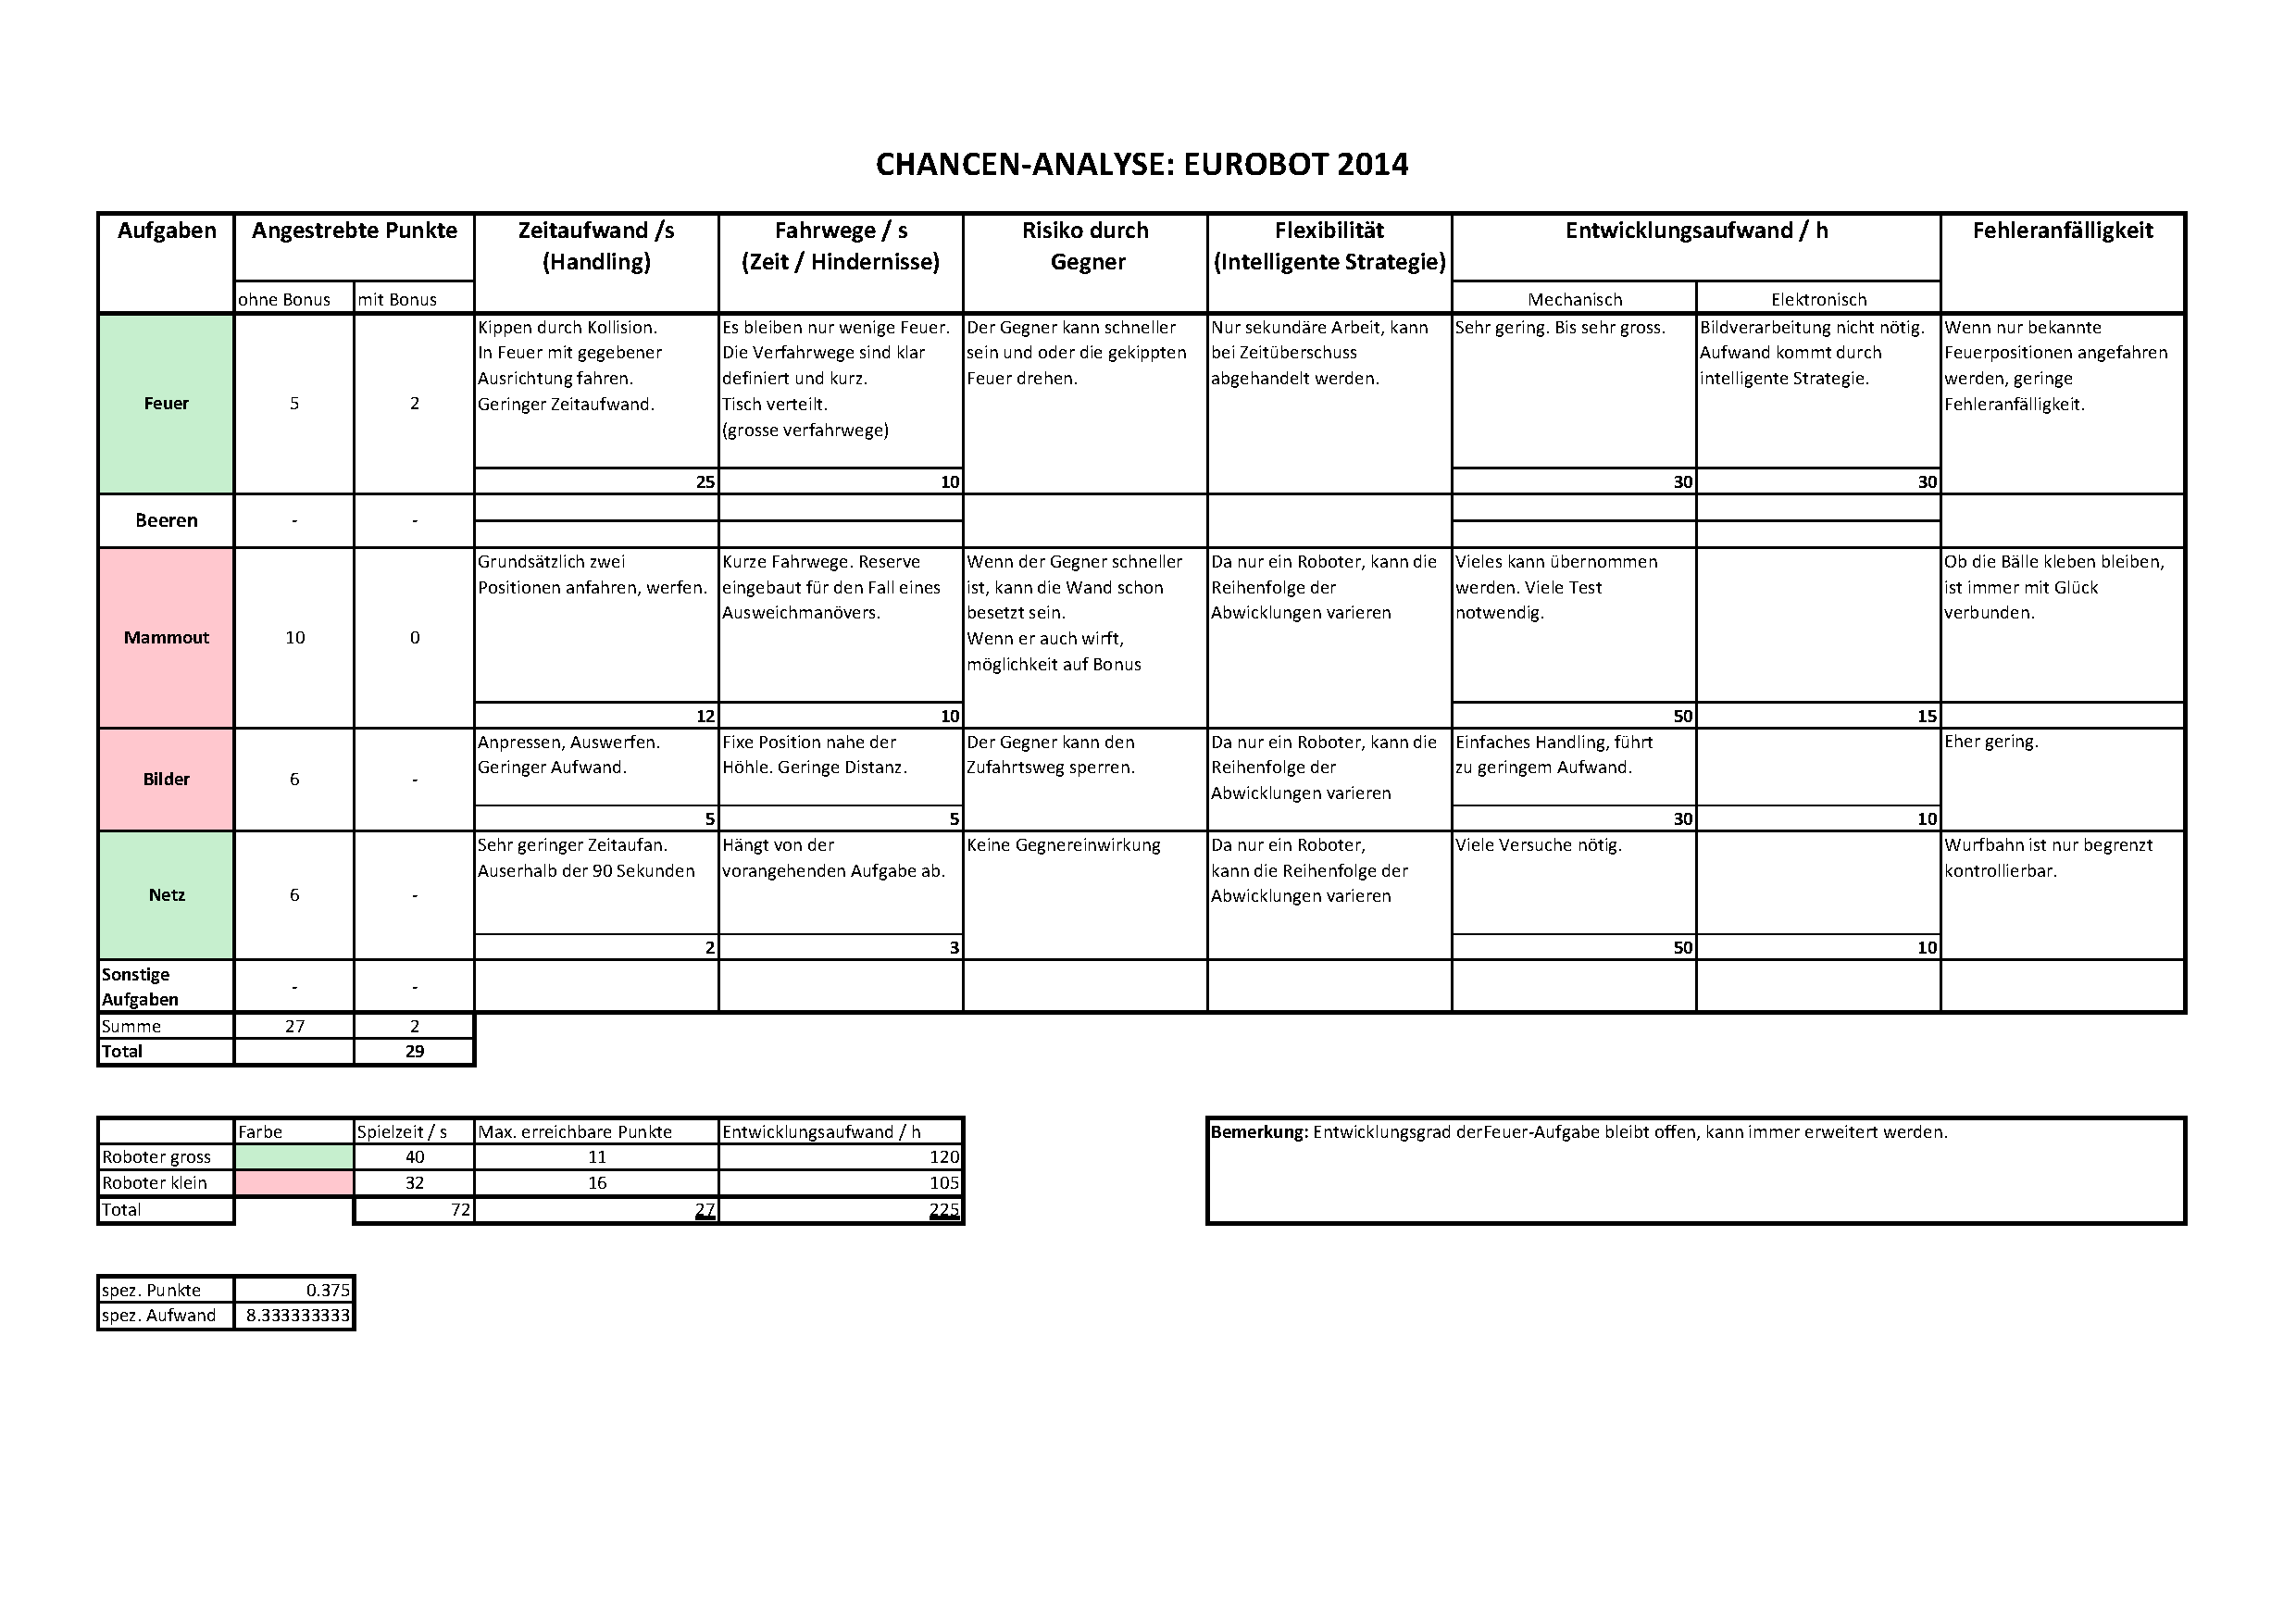
\includepdf[scale=0.7, pagecommand={}, pages=-, landscape=true]{appendix/image/c_strategie_1.pdf}
	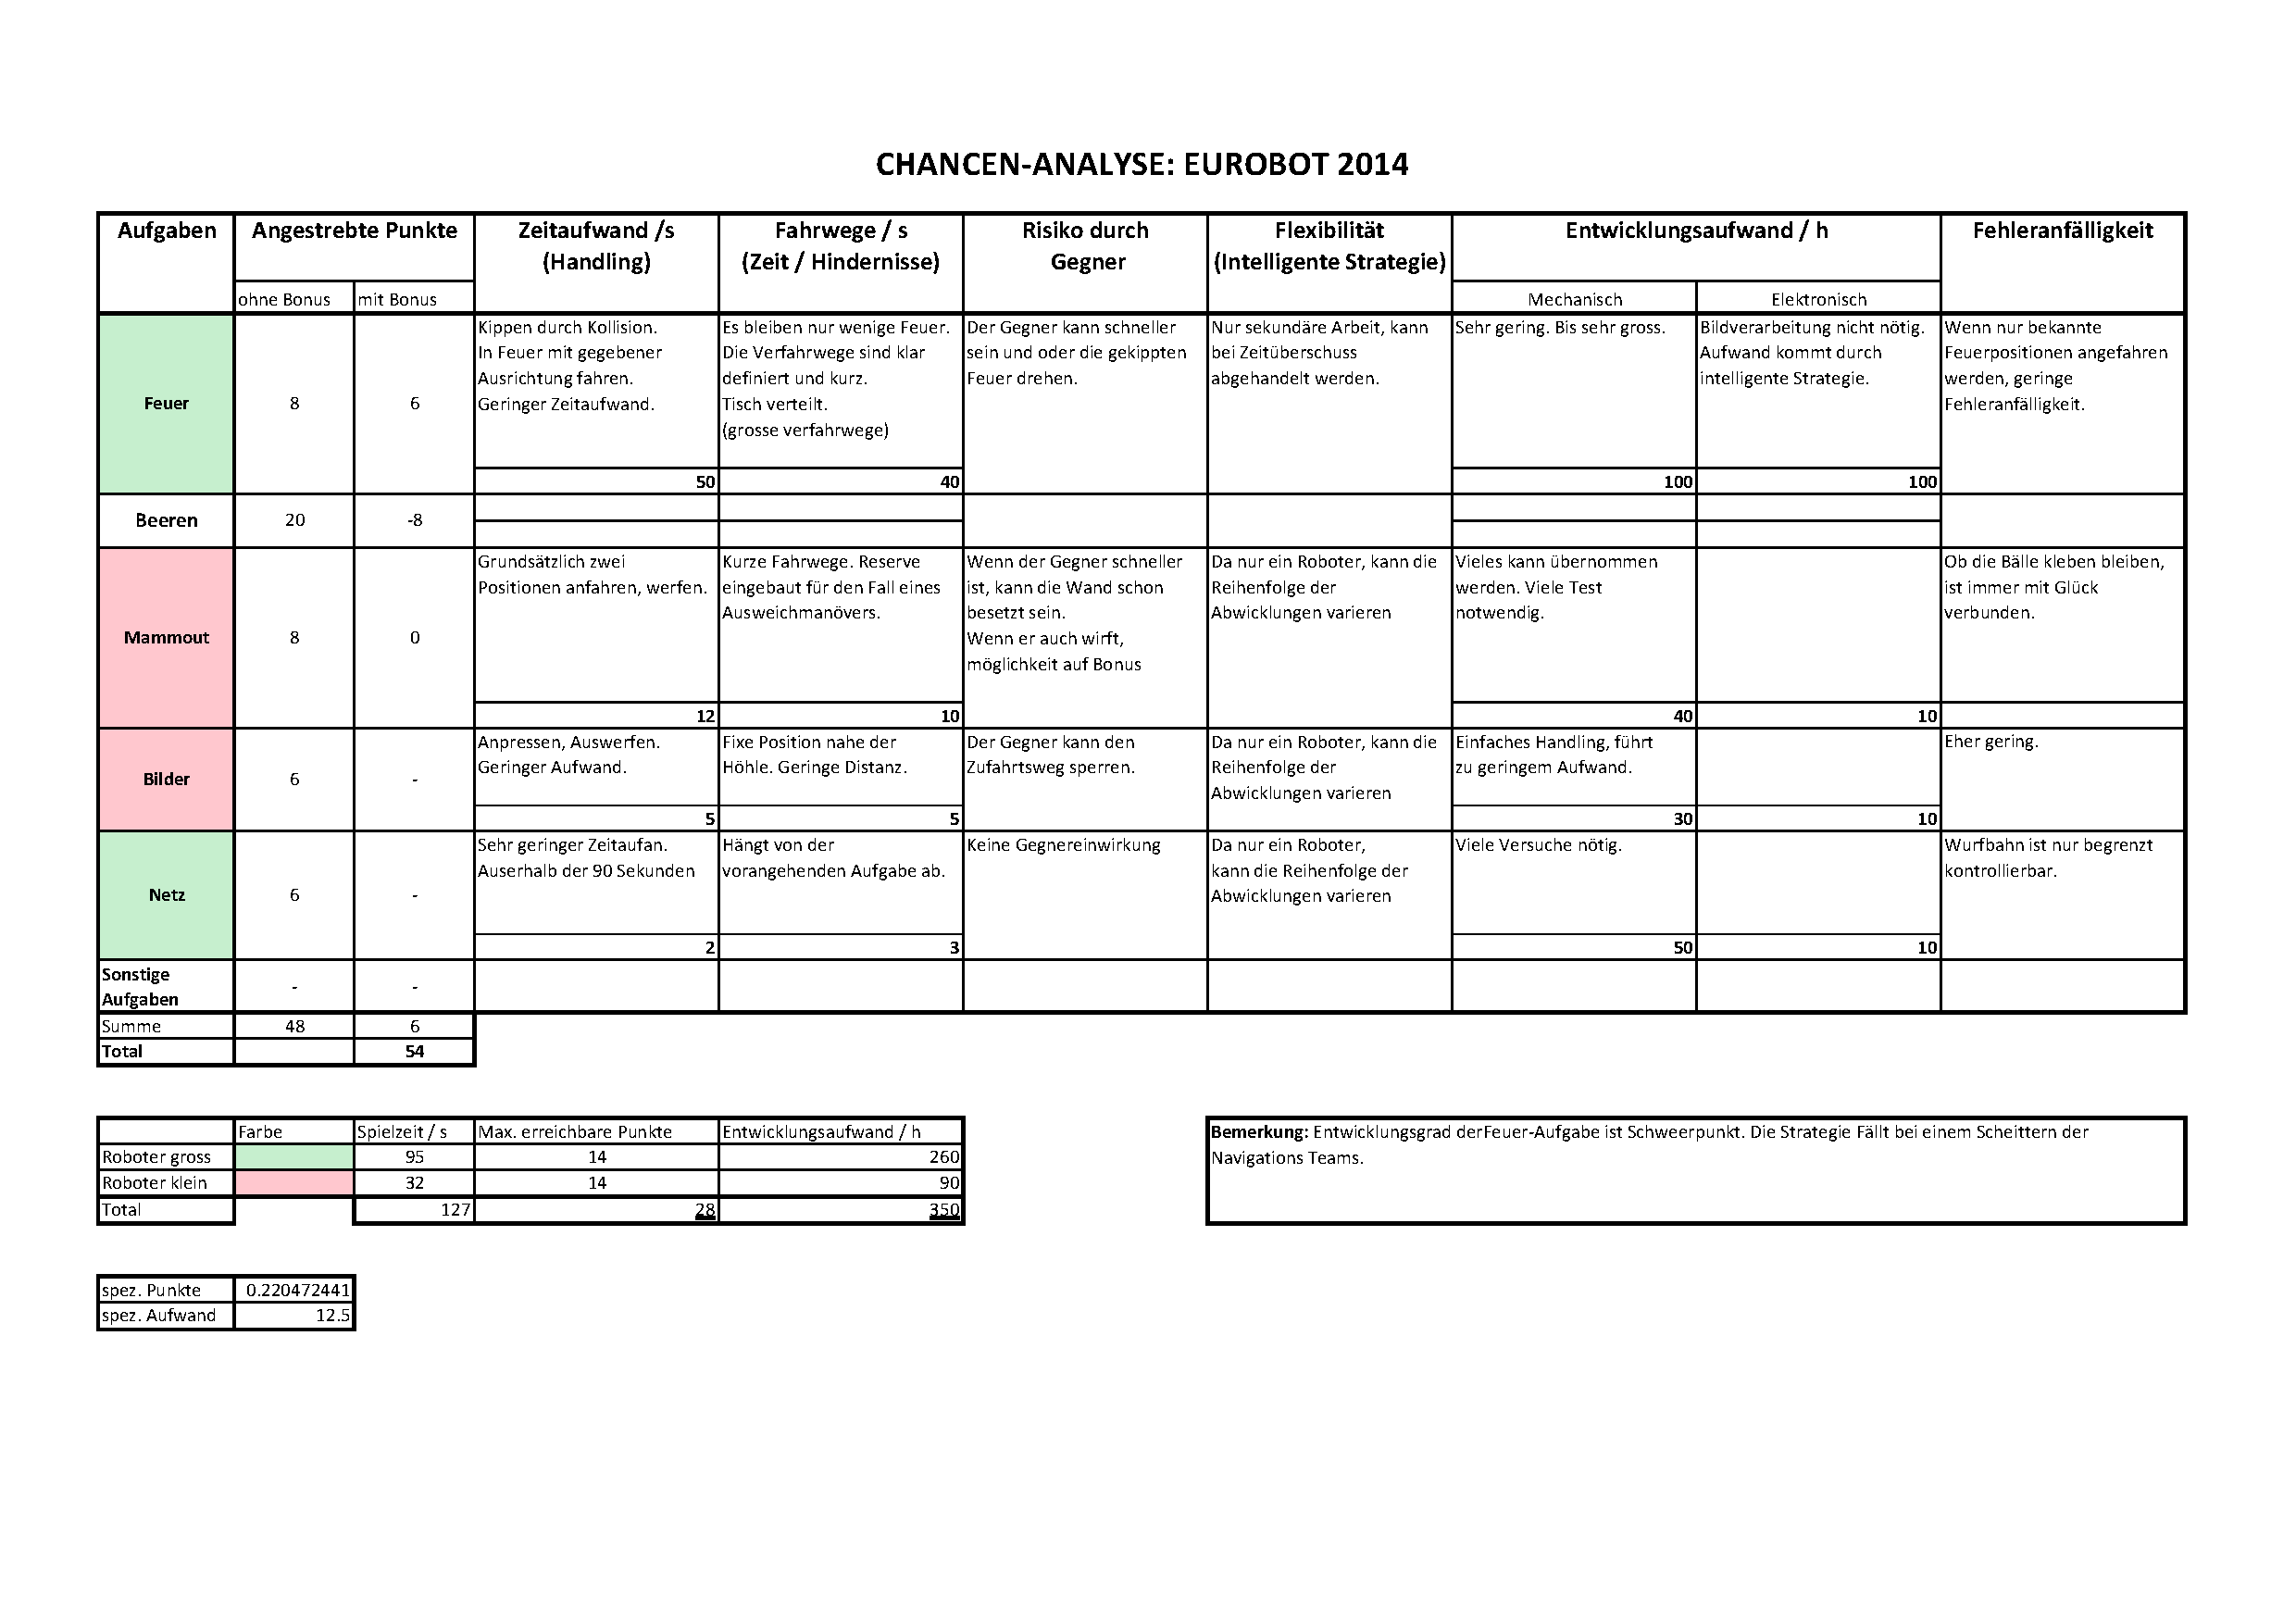
\includepdf[scale=0.7, pagecommand={}, pages=-, landscape=true]{appendix/image/c_strategie_2.pdf}
	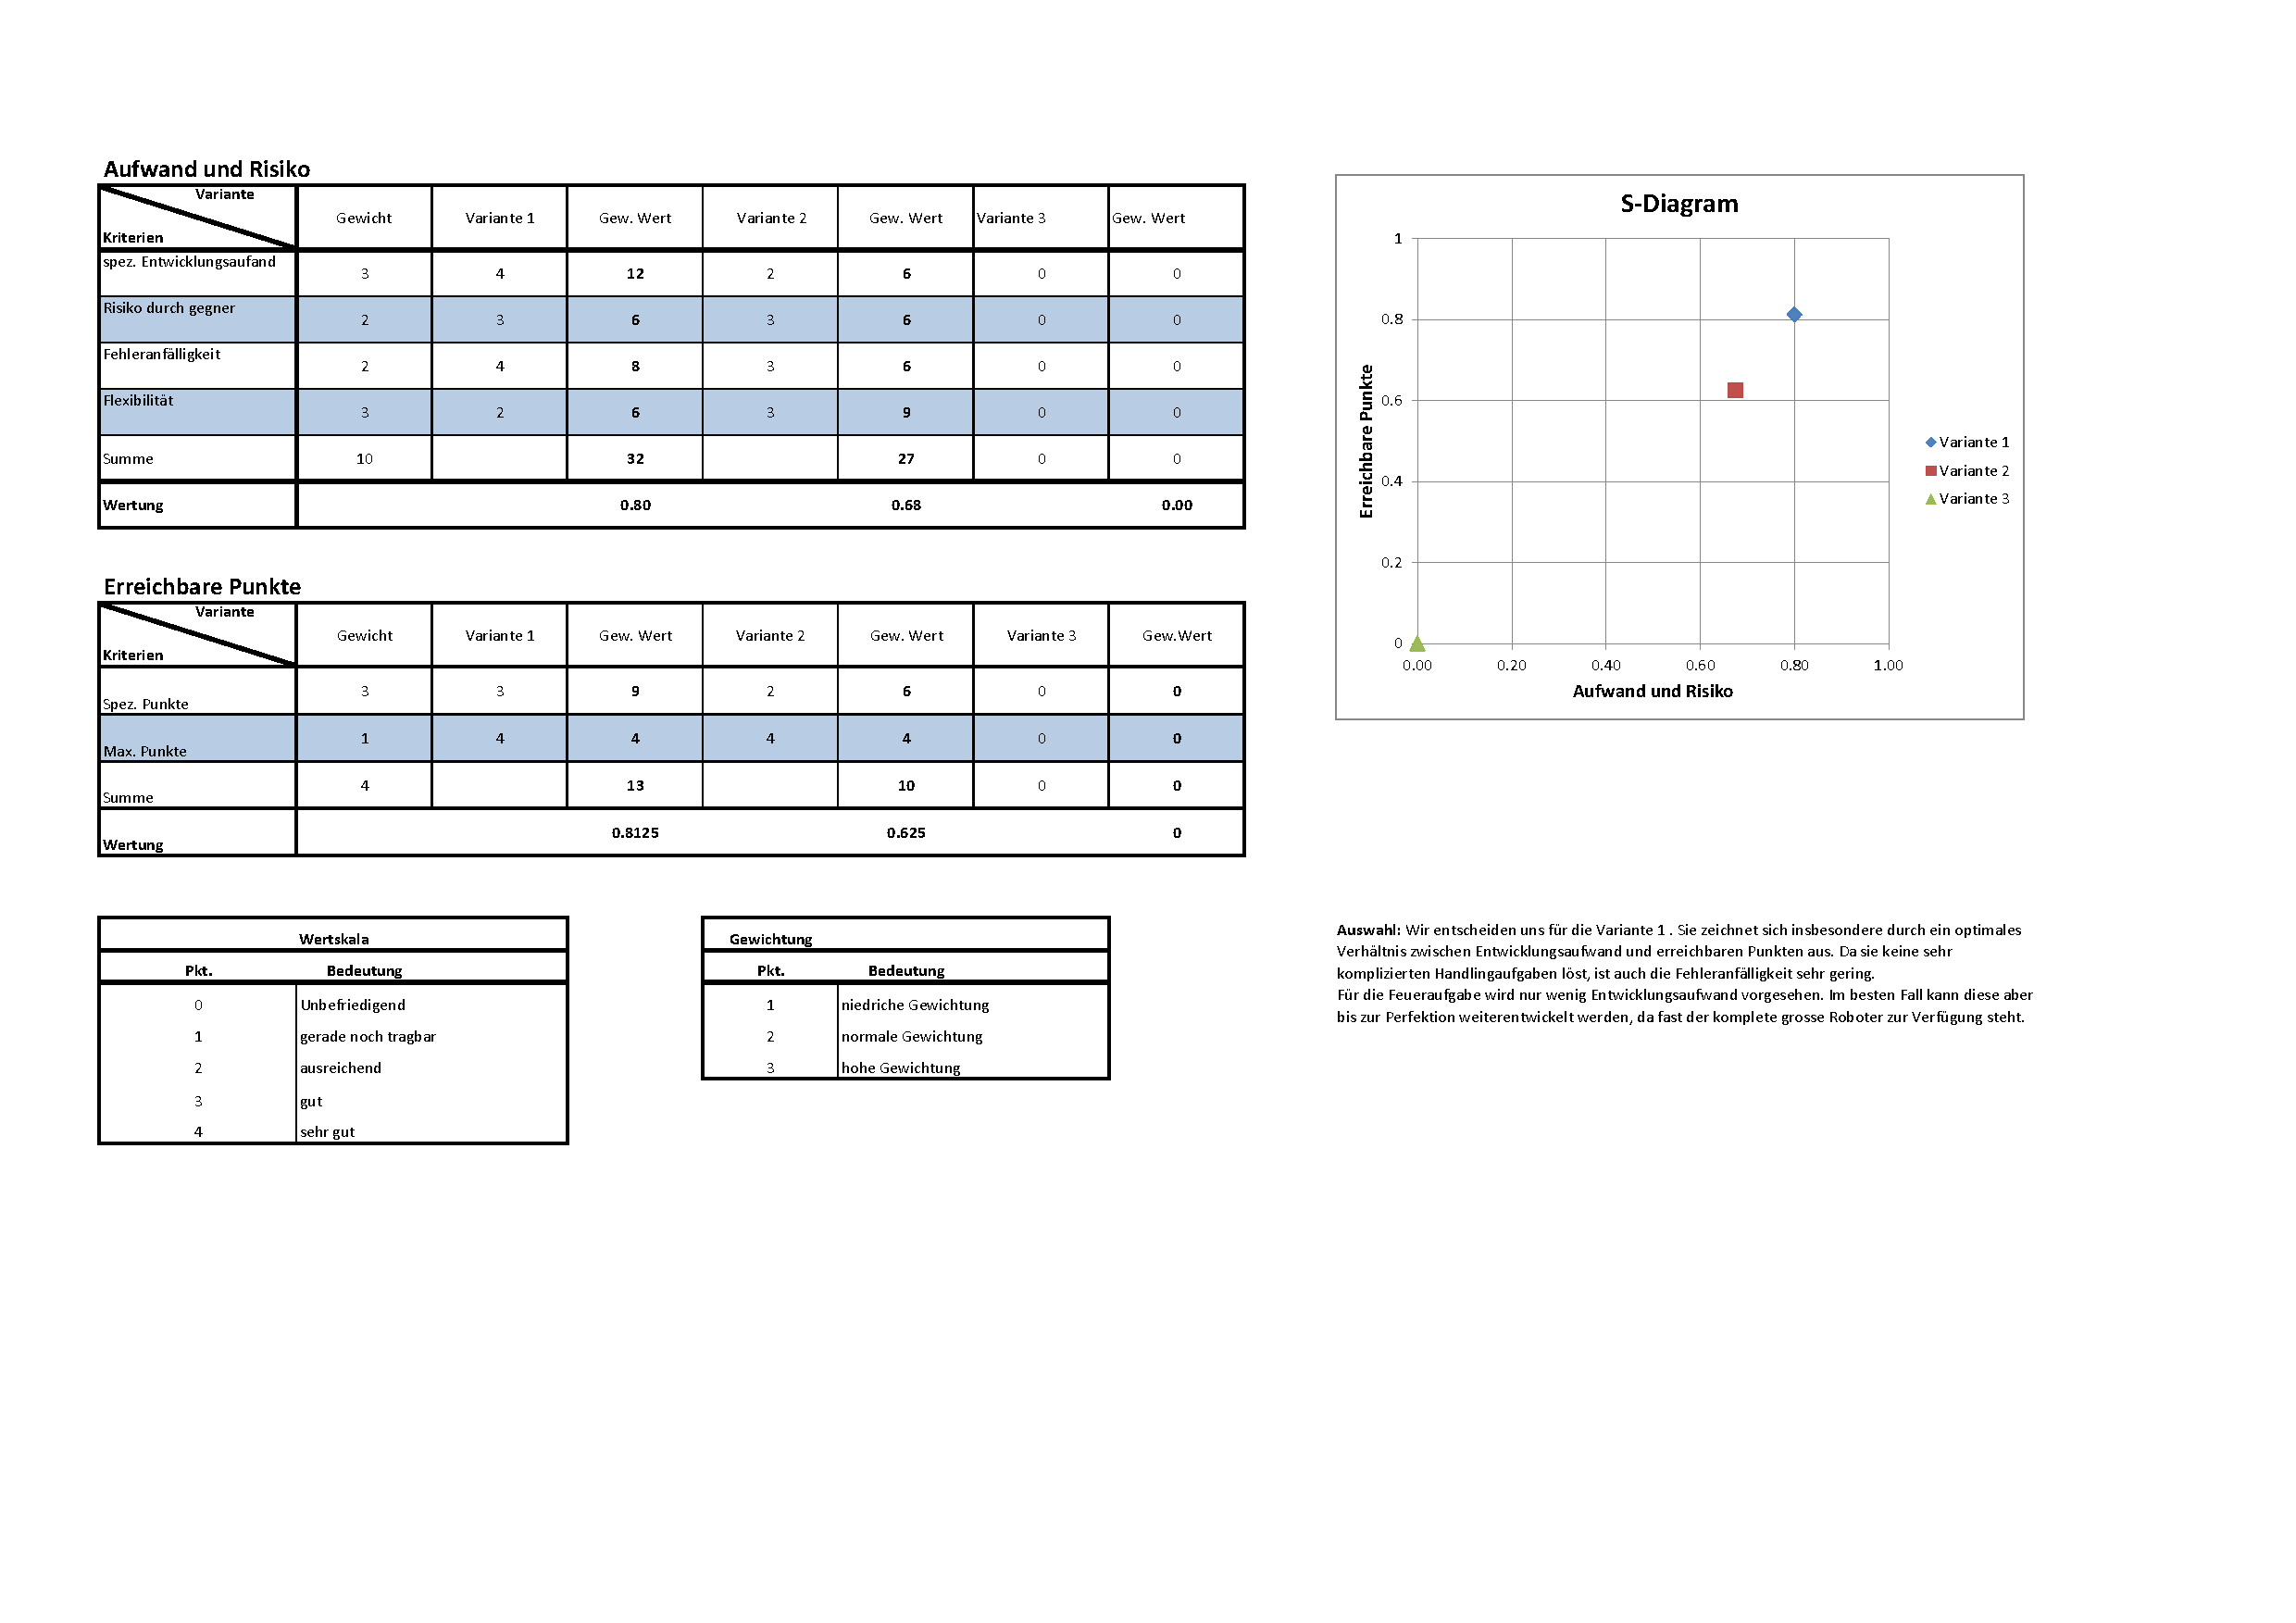
\includepdf[scale=0.7, pagecommand={}, pages=-, landscape=true]{appendix/image/c_s_diagramm.pdf}
    %
\includepdf[scale=0.85, pagecommand={\thispagestyle{plain}}, pages=-]{appendix/image/b_pflichtenheft.pdf}
    %
\includepdf[scale=0.85,pagecommand={\thispagestyle{plain}}, pages=-]{appendix/image/b_pflichtenheft.pdf}
%Anhang C
%%%%%%%%%%%%%%%%%%%%%%%%%%%%%%%%%%%%%%%%%%%%%%%%%%%%%%%%%%%%%%%%%%%%%%%%%%%%%%%
% Titel:   Bericht - Konzeptphase Mechanik
% Autor:   gross10
% Datum:   11.01.2014
% Version: 0.0.1
%%%%%%%%%%%%%%%%%%%%%%%%%%%%%%%%%%%%%%%%%%%%%%%%%%%%%%%%%%%%%%%%%%%%%%%%%%%%%%%
%
%:::Change-Log:::
% Versionierung erfolgt auf folgende Gegebenheiten: -1. Release Versionen
%                                                   -2. Neue Kapitel
%                                                   -3. Fehlerkorrekturen
%
% 0.0.01      Erstellung der Datei
%%%%%%%%%%%%%%%%%%%%%%%%%%%%%%%%%%%%%%%%%%%%%%%%%%%%%%%%%%%%%%%%%%%%%%%%%%%%%%% 
\chapter{Konzeptphase Mechanik}\label{ch:konzeptphase_mechanik}
	Dieser Anhang beinhaltet die Konzepte der Spielaufgaben \gls{g:fresko} und \gls{g:mammut}.
	\paragraph{PA1}
	\begin{itemize}
		\item Morphologischer Kasten \gls{g:fresko}
		\item Morphologischer Kasten \gls{g:mammut}
		\item Testprotokolle
		\item Nutzwertanalyse
		\item Abschlusswinkel
		\item Verformung
	\end{itemize}
	%
	\paragraph{PA2}
	\begin{itemize}
		\item Morphologischer Kasten \gls{g:mammut_catch}
		\item Morphologischer Kasten \gls{g:fire}
		\item Testprotokolle
		\item S-Diagramm Netz
		\item Mathcad-Berechnung-Servos
	\end{itemize}
	%
%PA1
    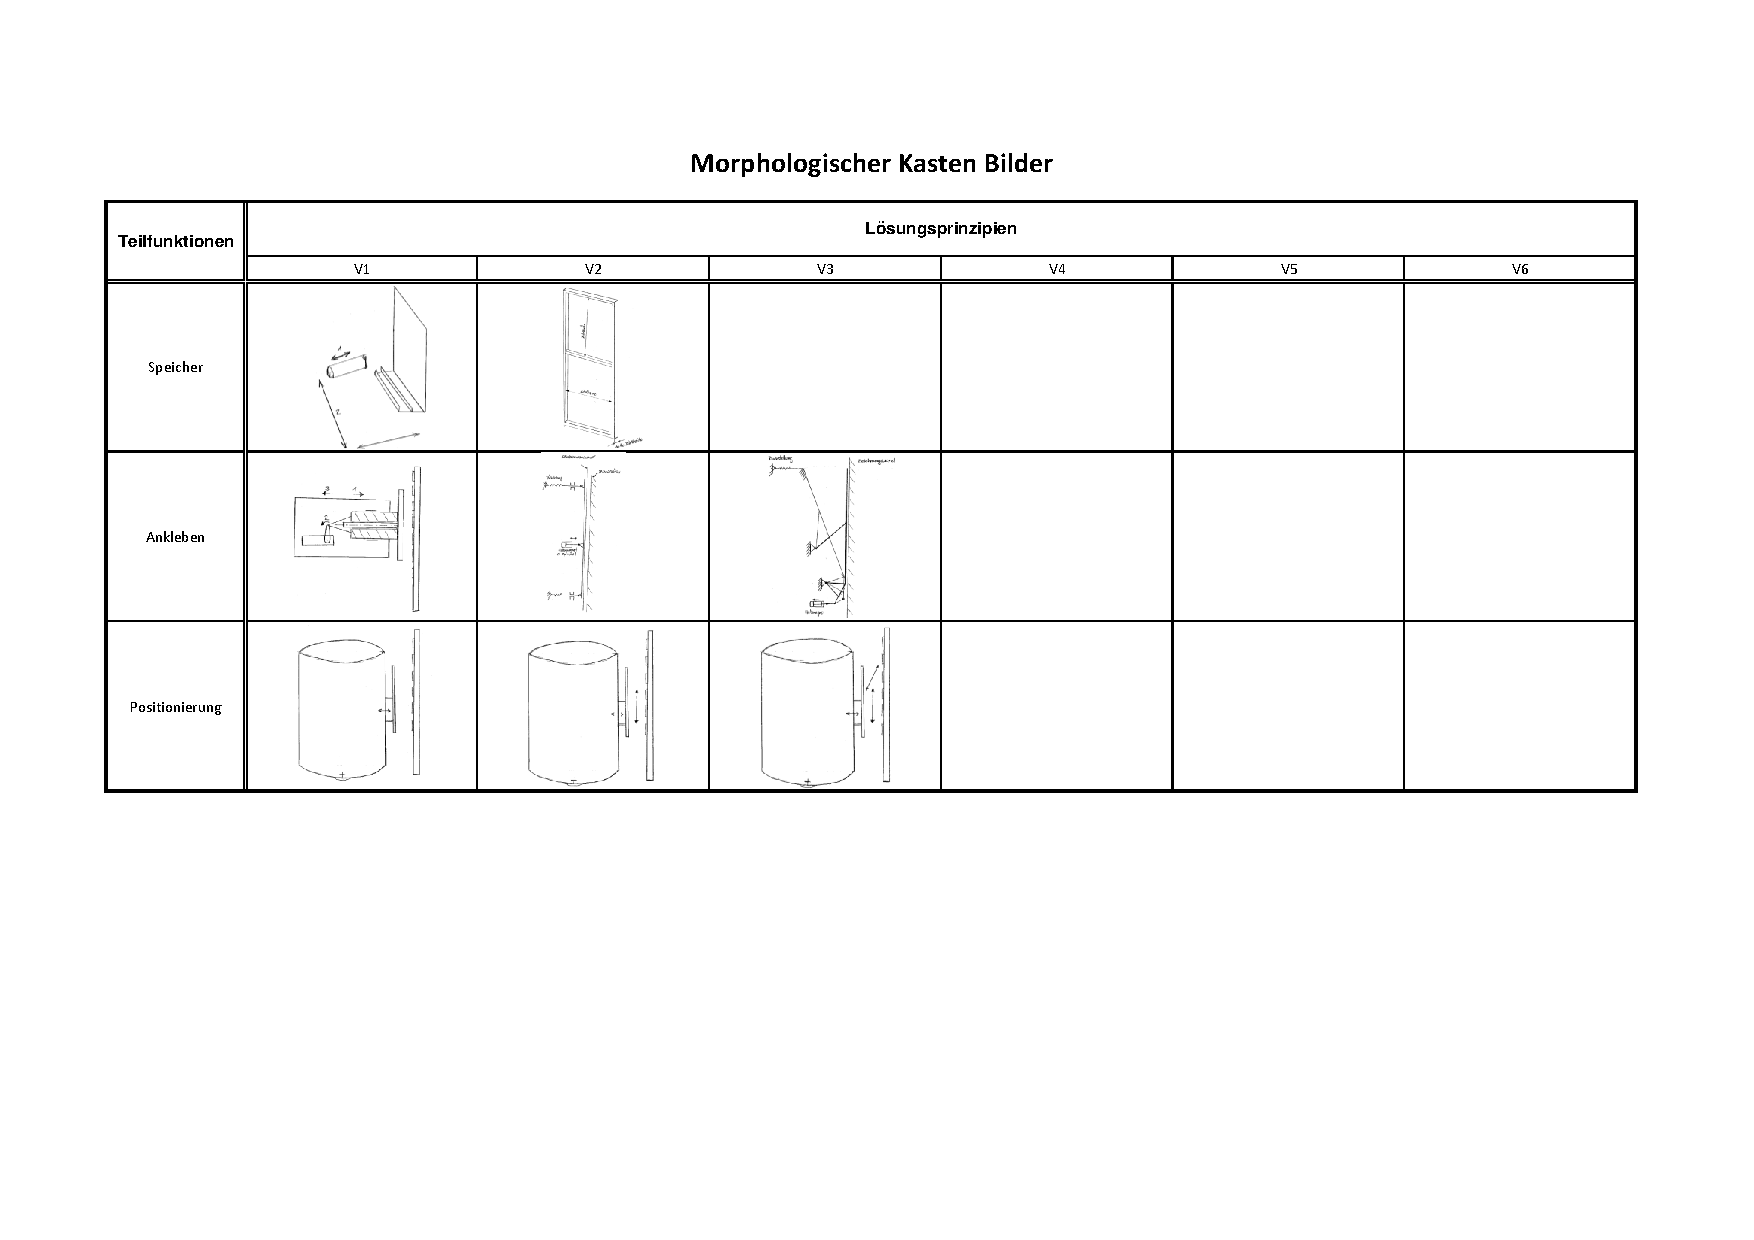
\includepdf[scale=0.80, pagecommand={}, pages=-, landscape=true]{appendix/image/d_Morph_Kast_Bilder.pdf}
    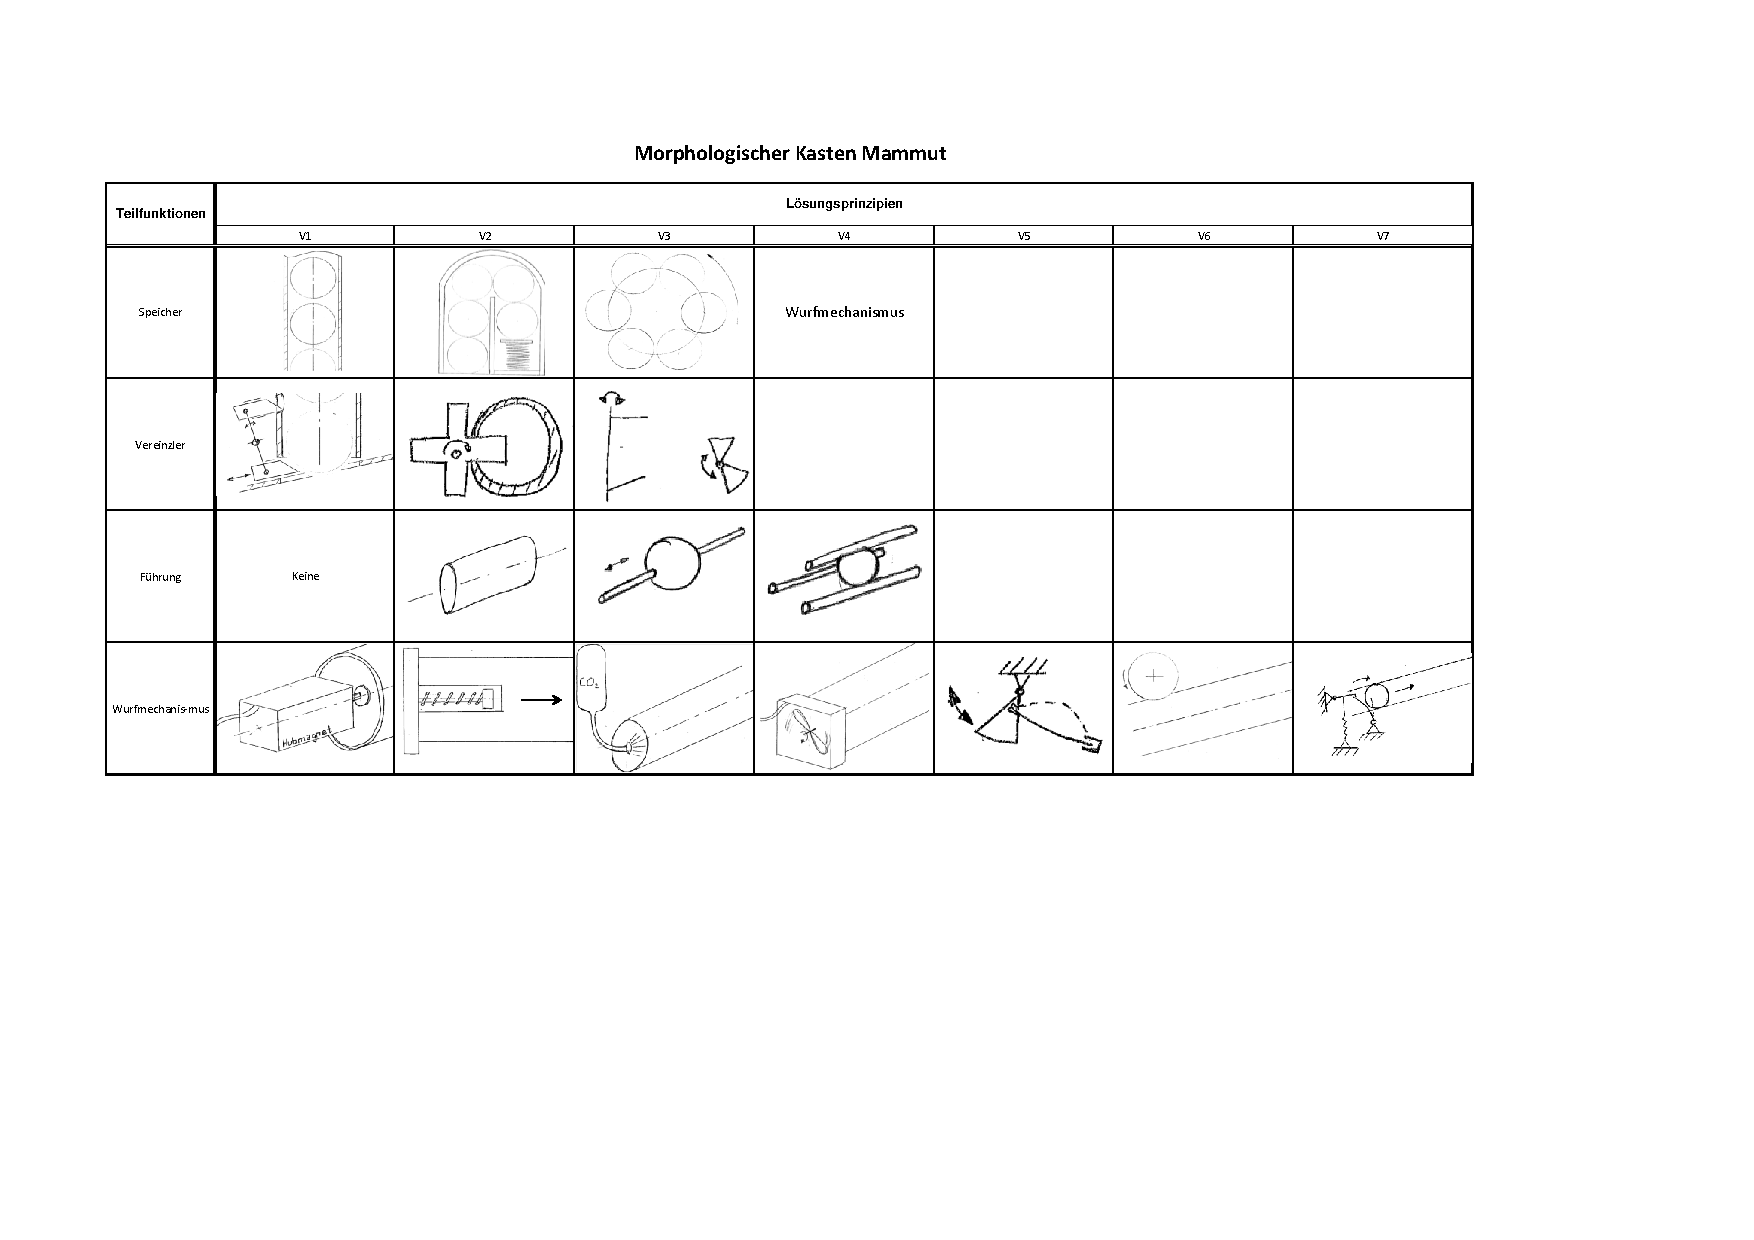
\includepdf[scale=0.80, pagecommand={}, pages=-, landscape=true]{appendix/image/d_Morph_Kast_Mammut.pdf}
    %
    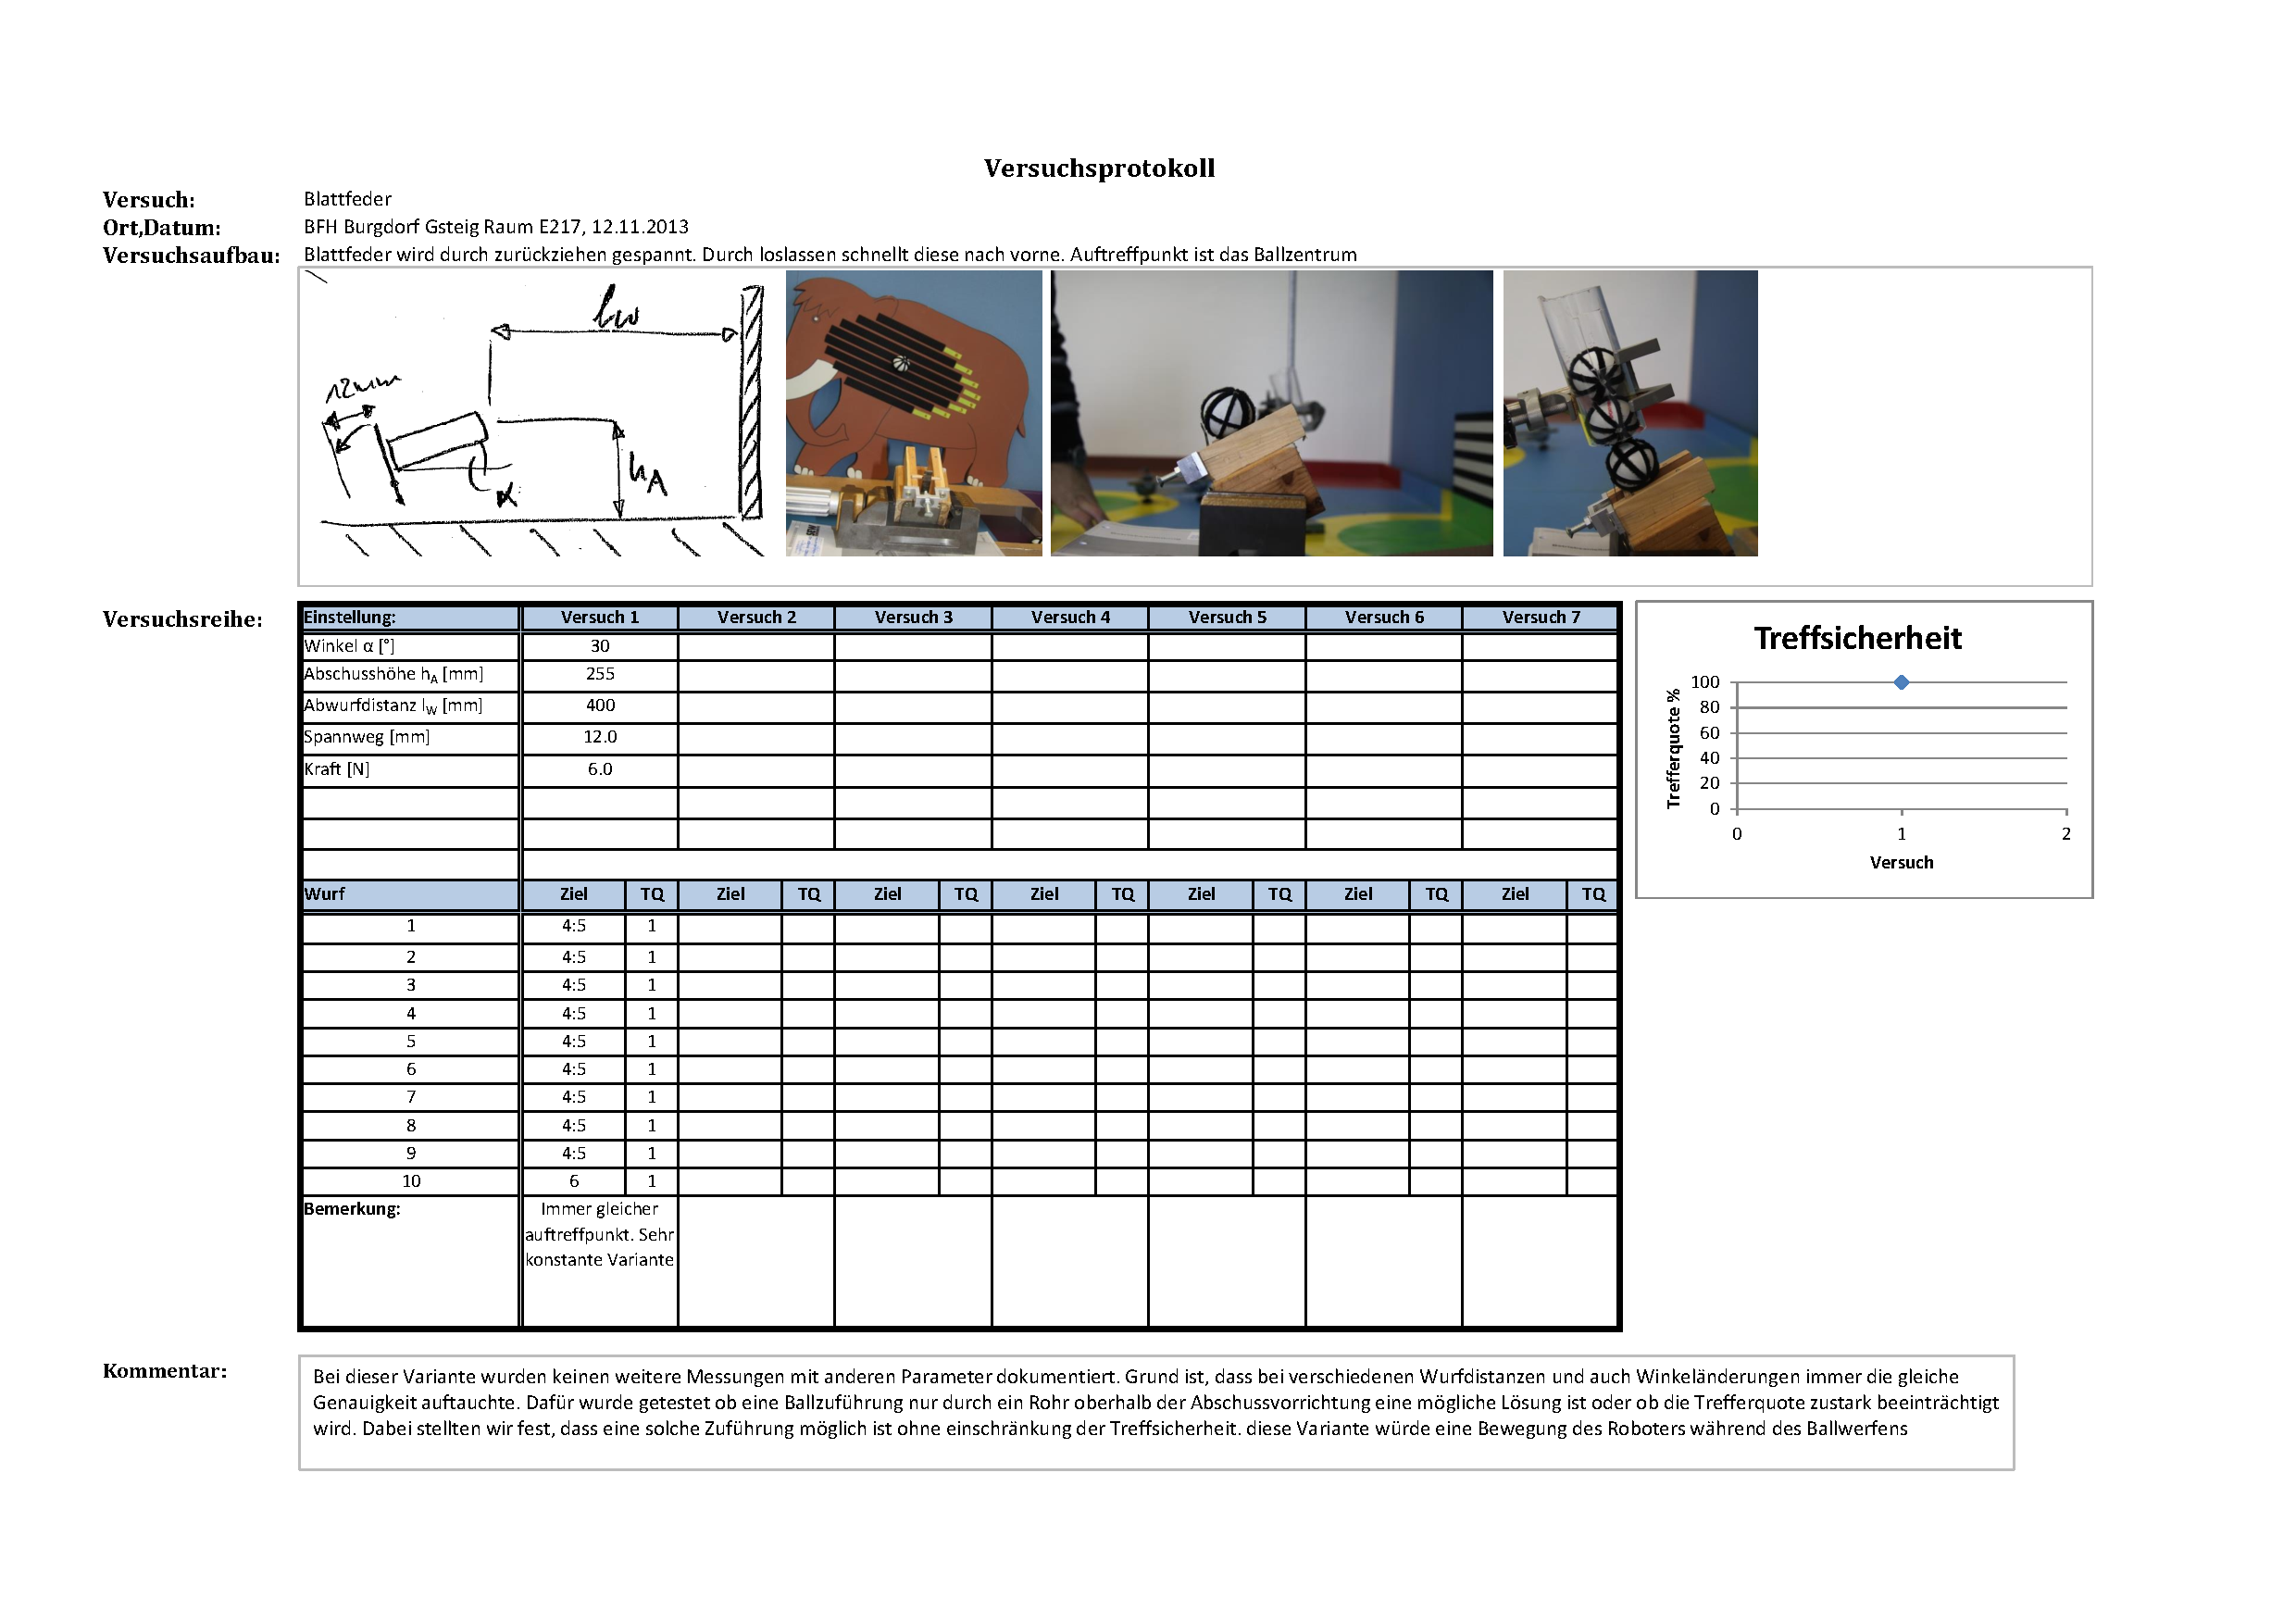
\includepdf[scale=0.80, pagecommand={}, pages=-, landscape=true]{appendix/image/d_Testprotokoll_Blattfeder.pdf}
    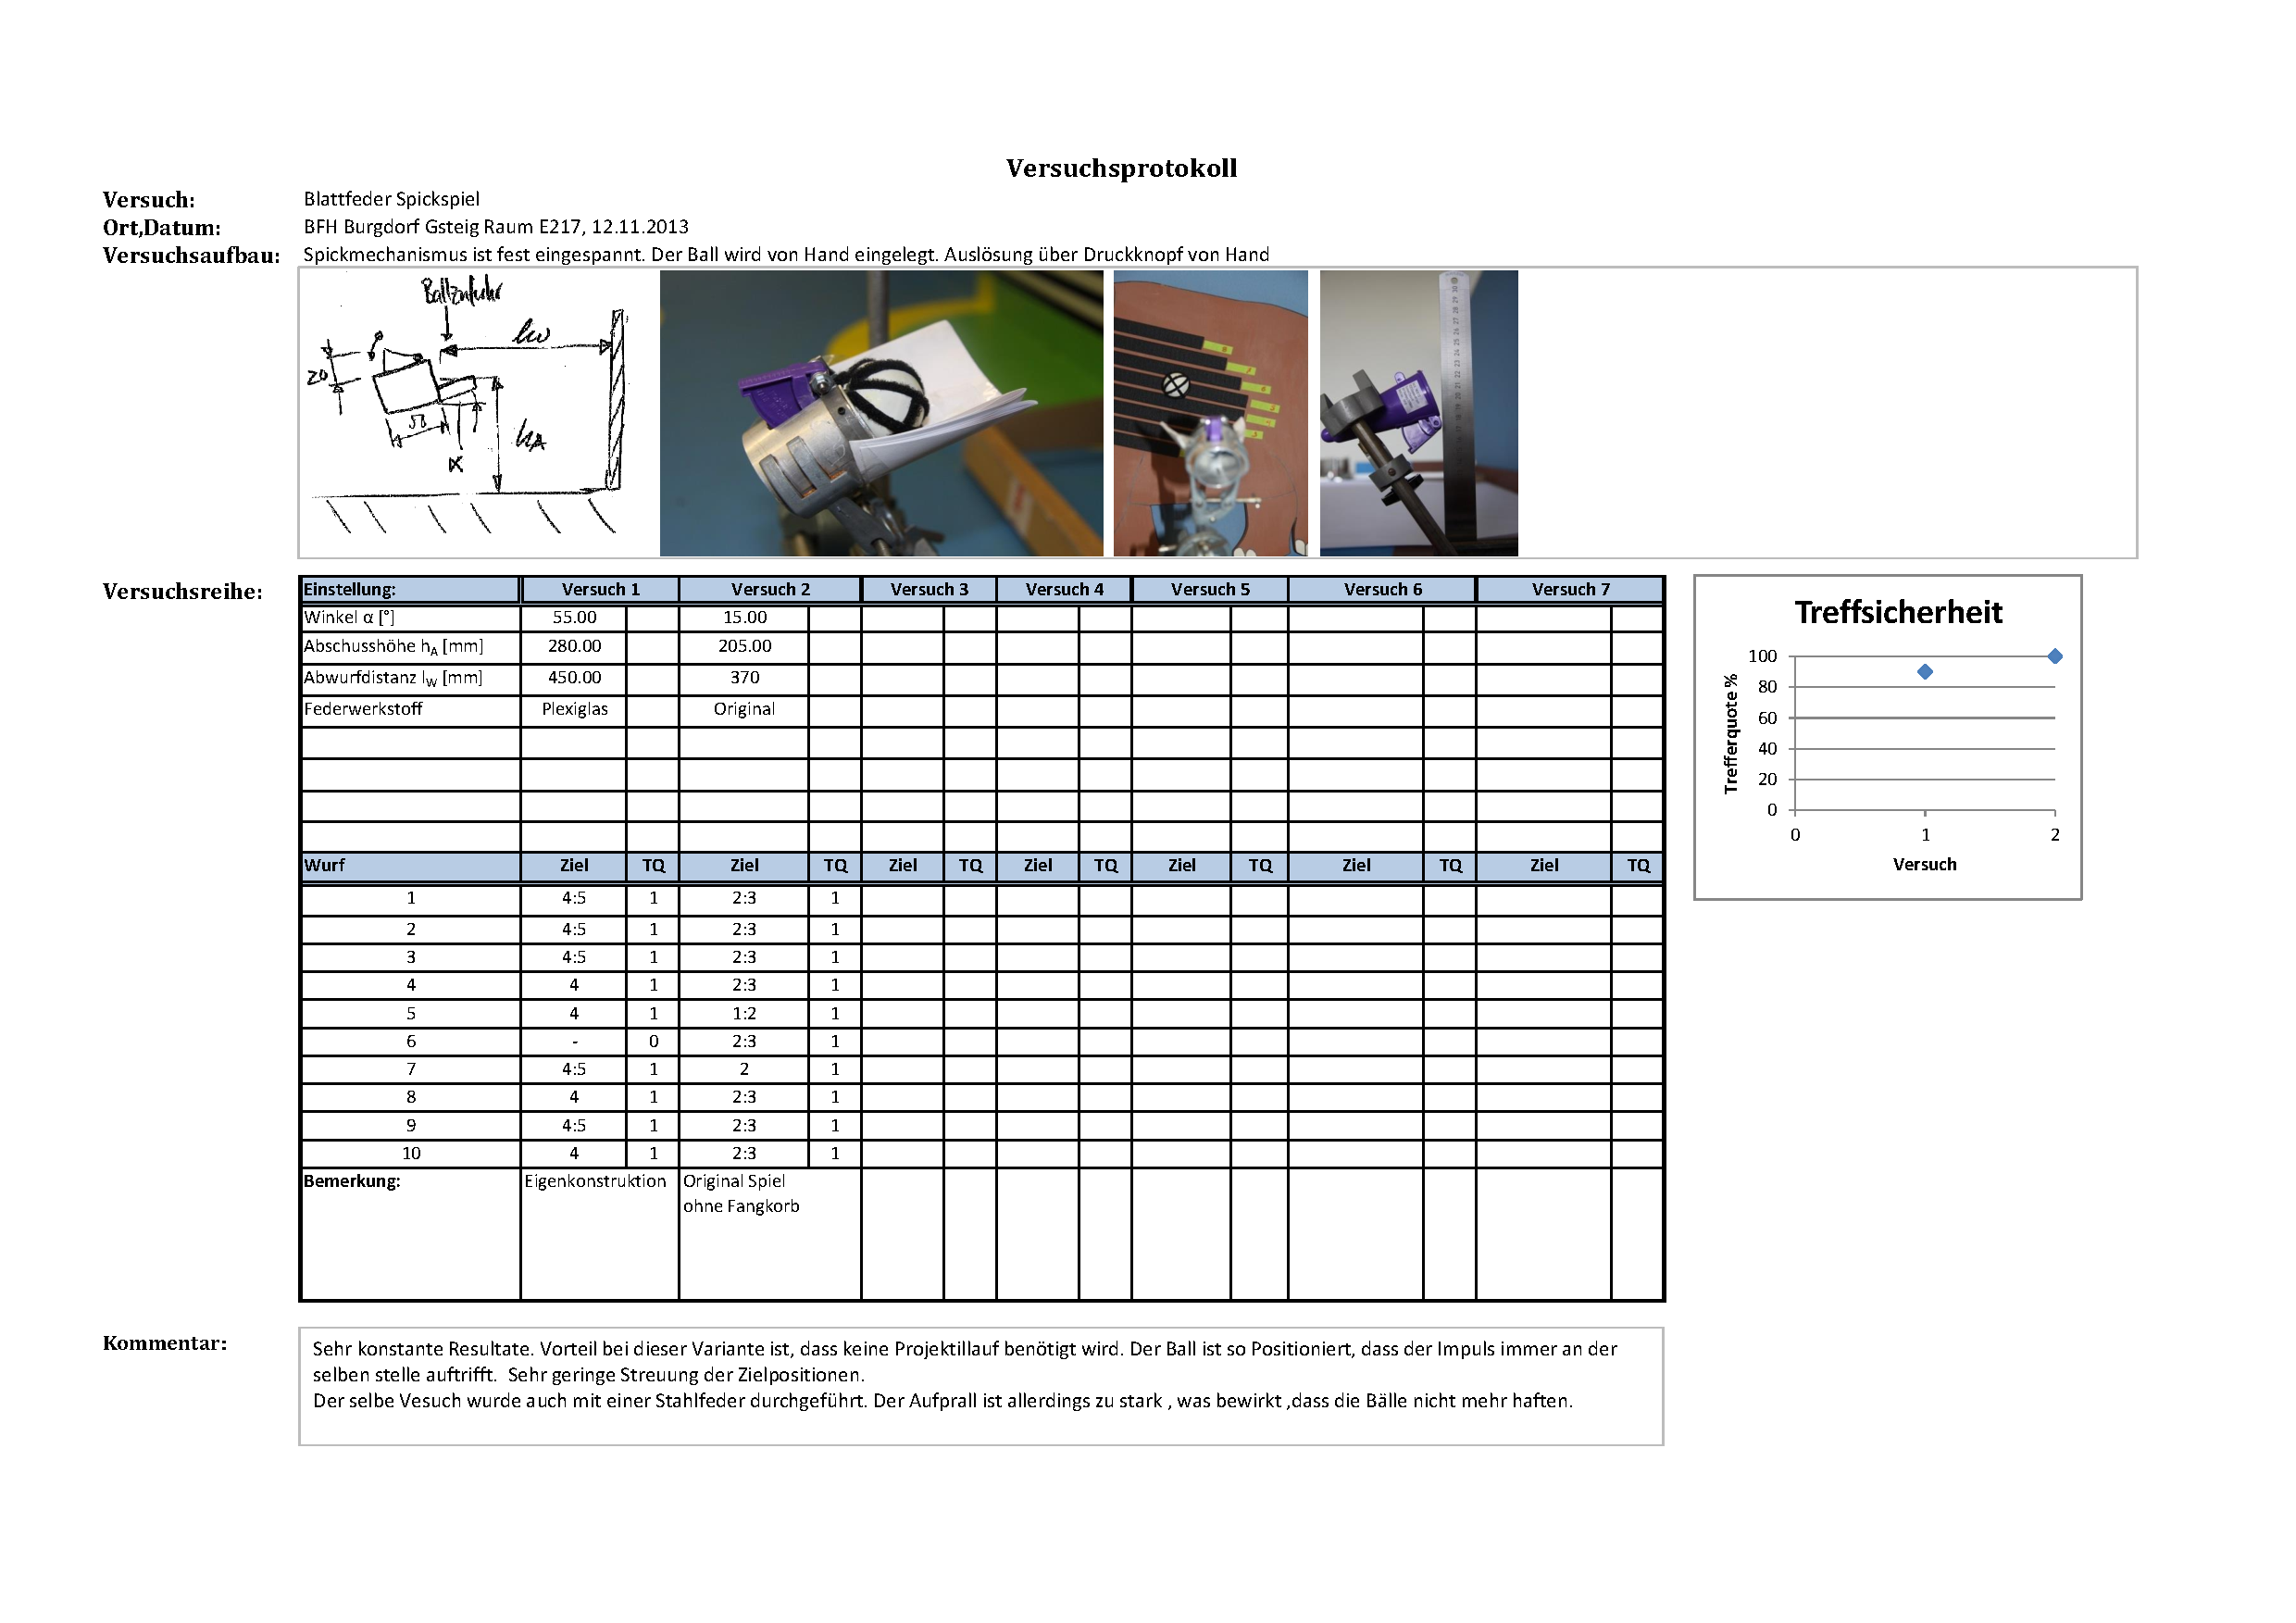
\includepdf[scale=0.80, pagecommand={}, pages=-, landscape=true]{appendix/image/d_Testprotokoll_Blattfeder_Spickspiel.pdf}
    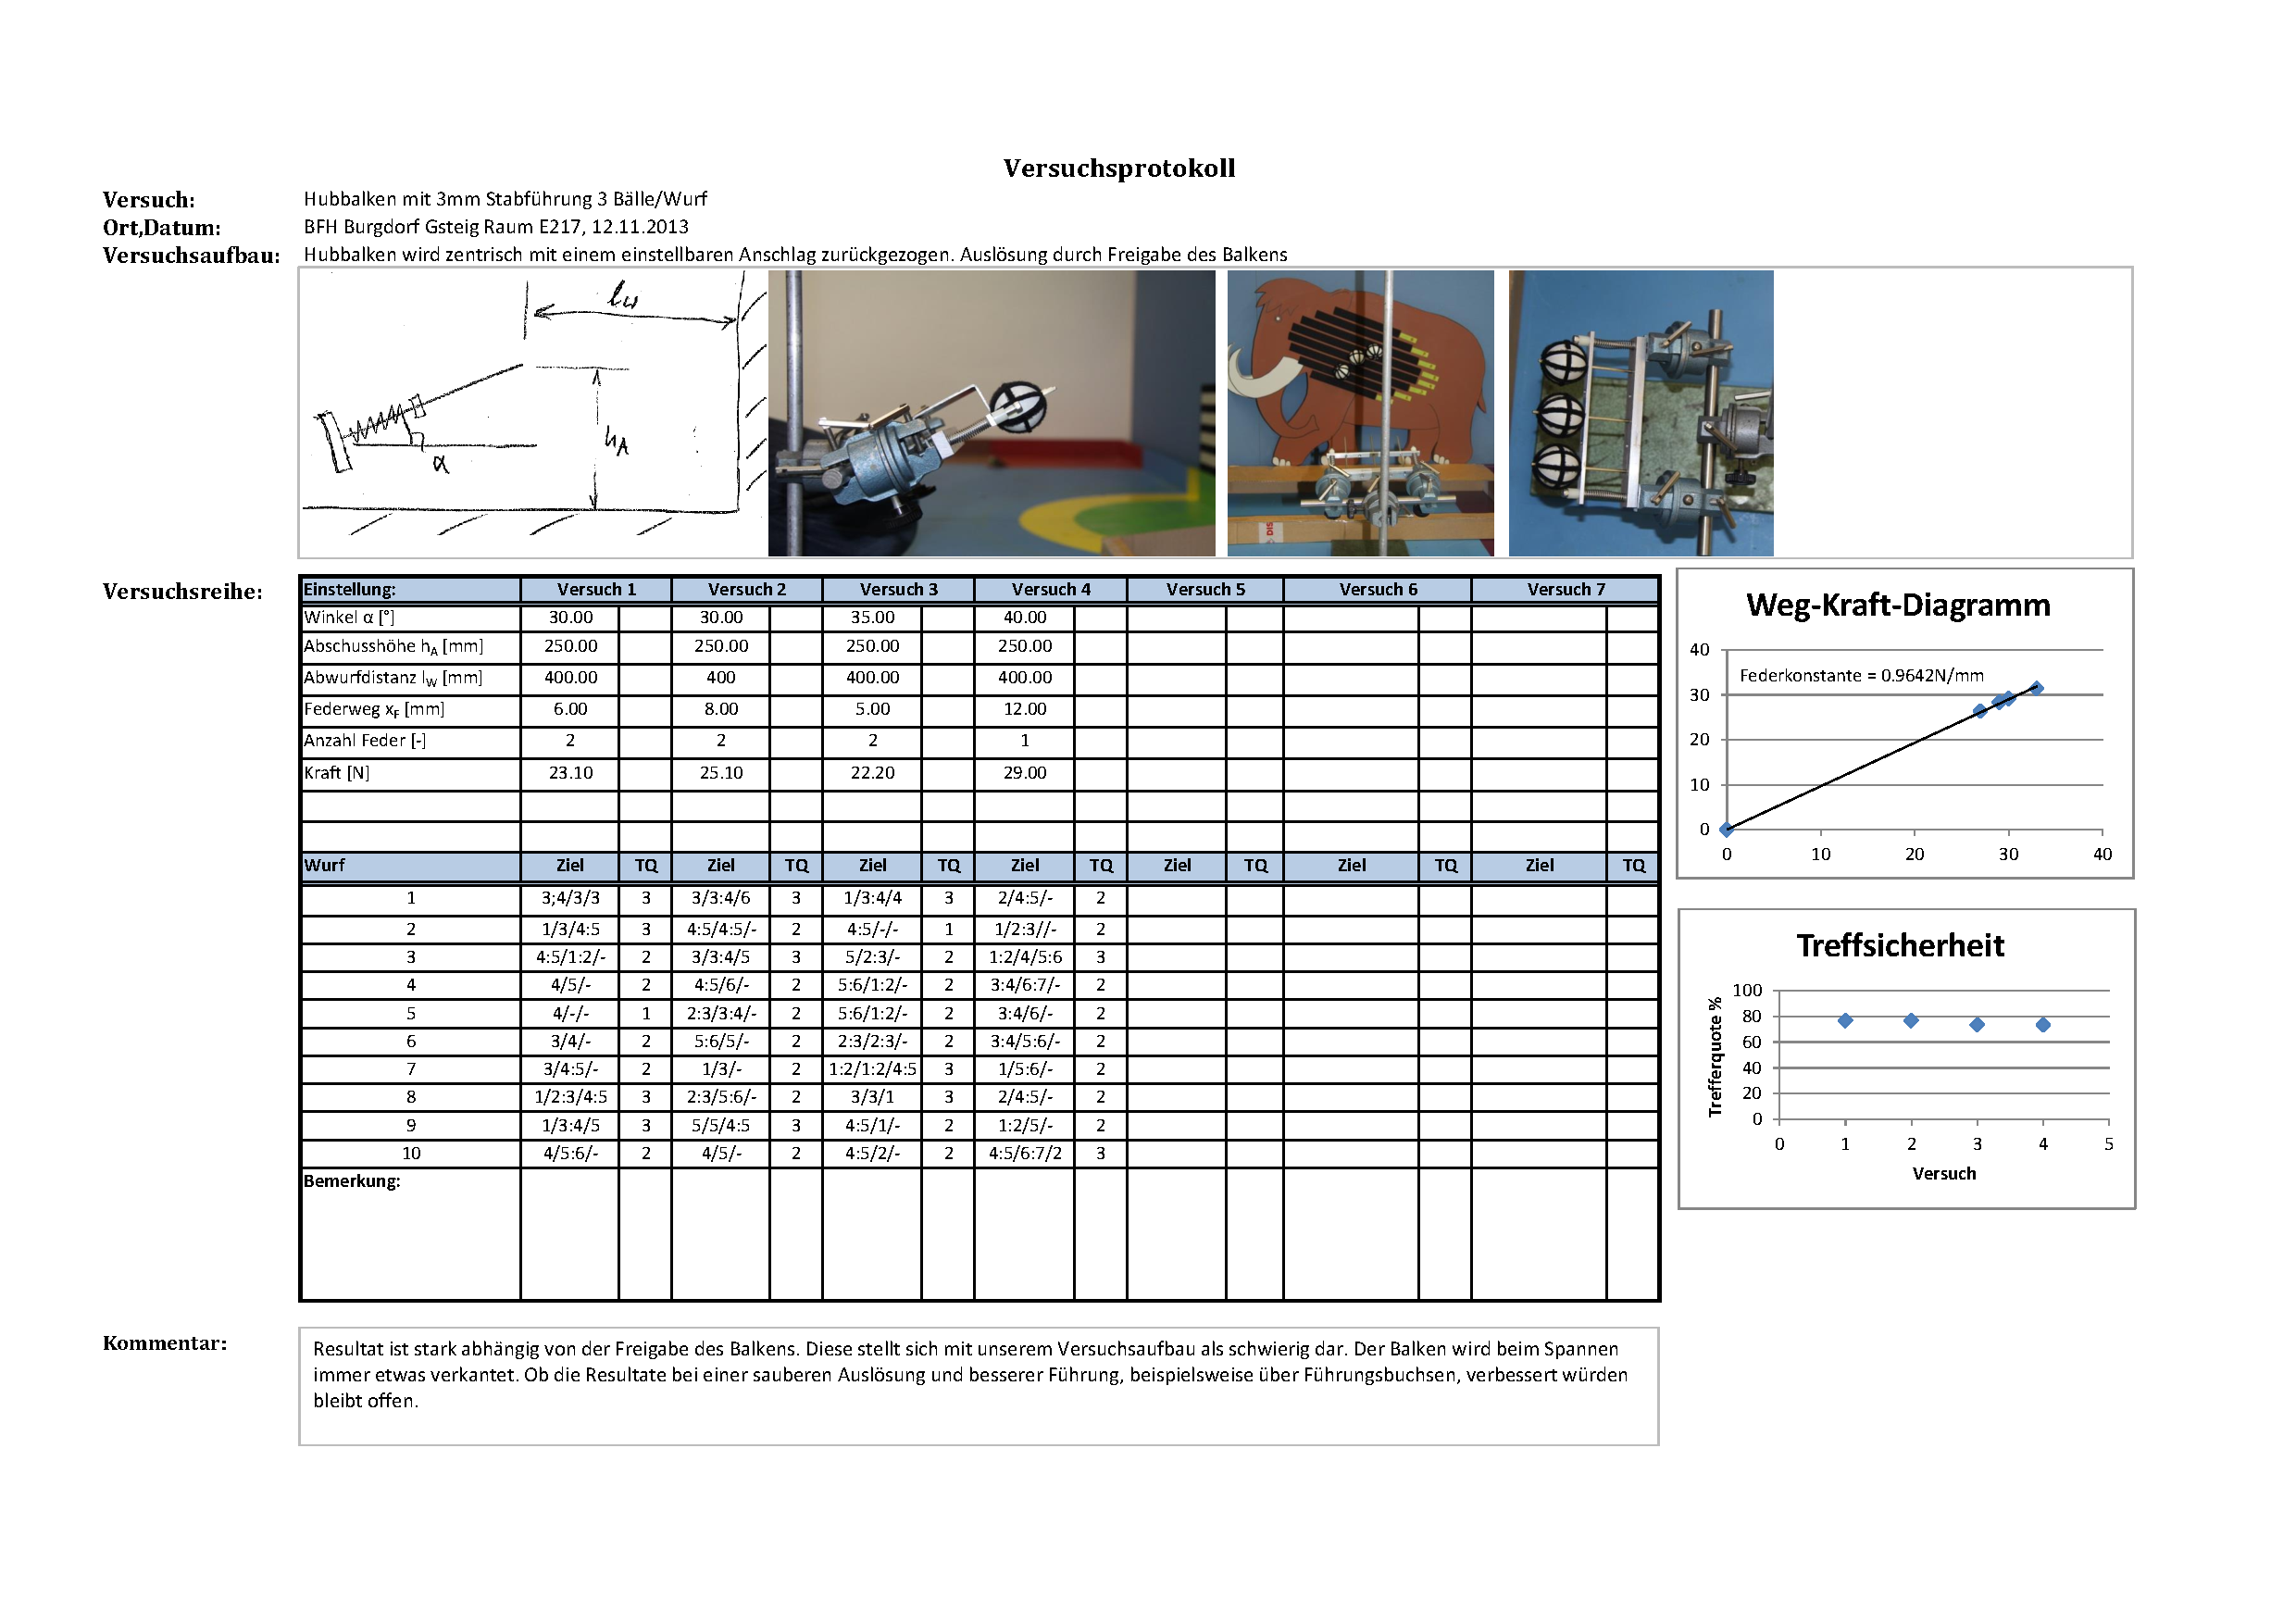
\includepdf[scale=0.80, pagecommand={}, pages=-, landscape=true]{appendix/image/d_Testprotokoll_Hubbalken_mit_3mm_Stabfuehrung.pdf}
    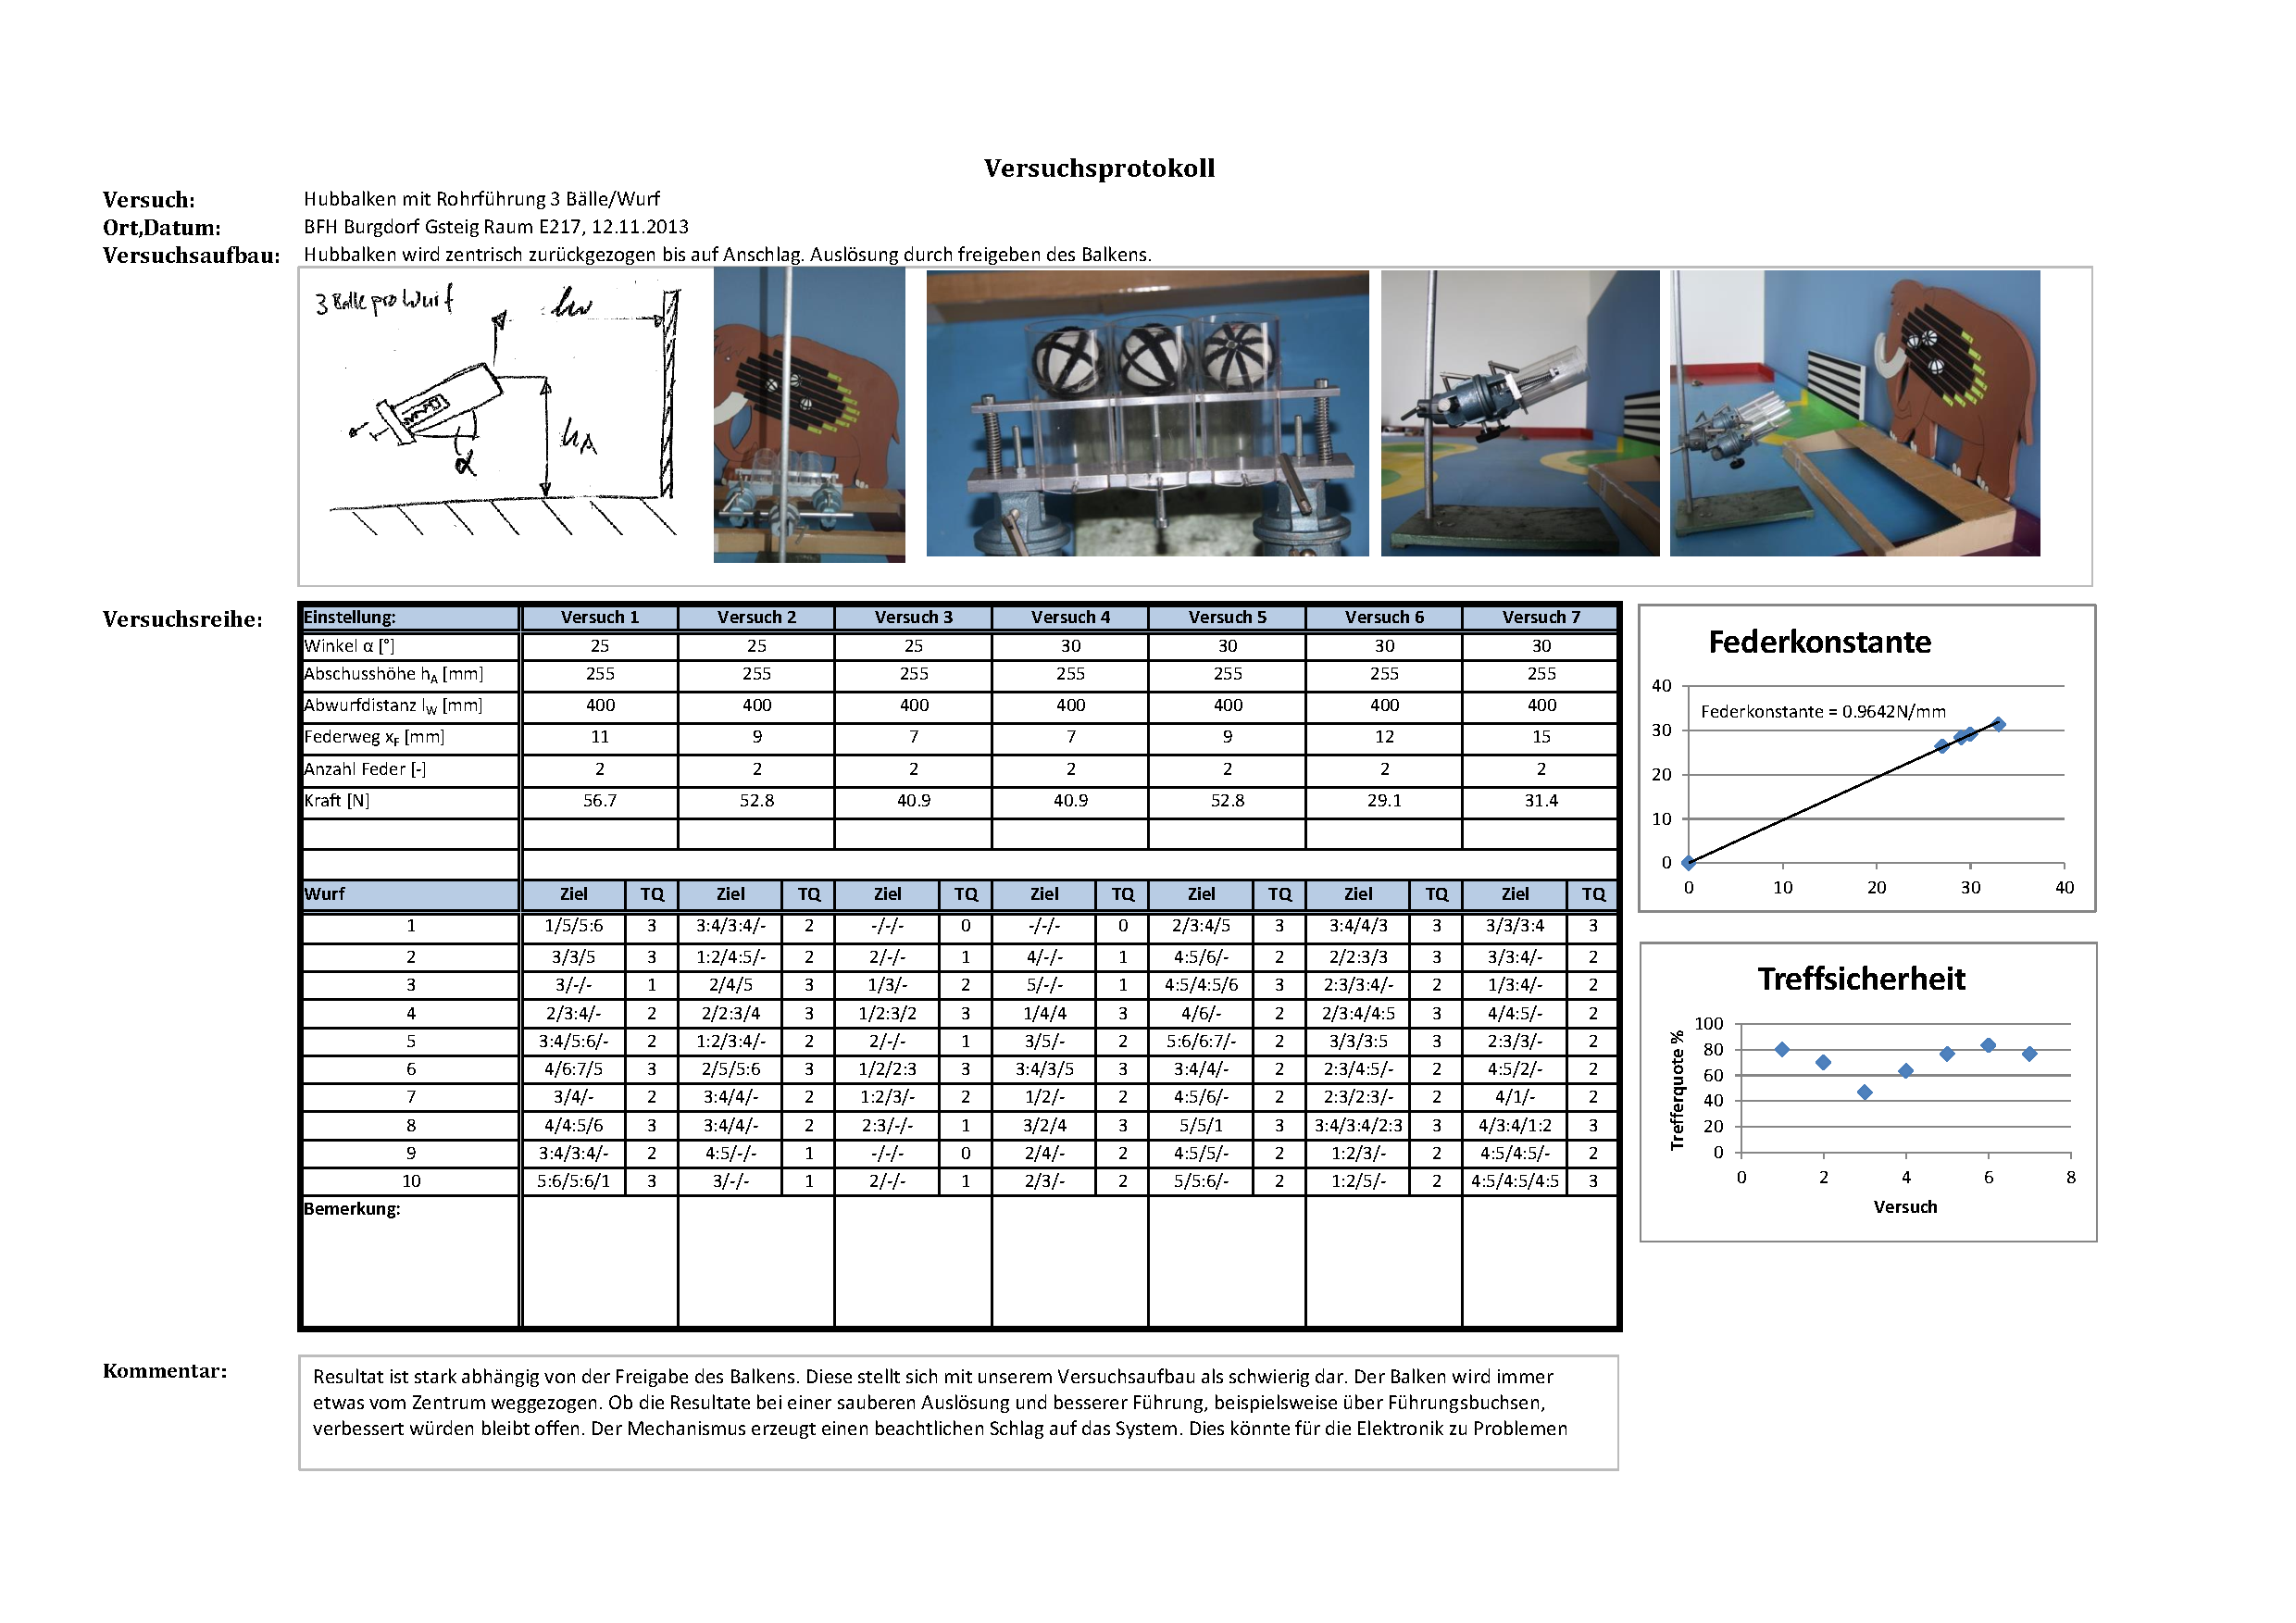
\includepdf[scale=0.80, pagecommand={}, pages=-, landscape=true]{appendix/image/d_Testprotokoll_Hubbalken_Rohrfuehrung.pdf}
    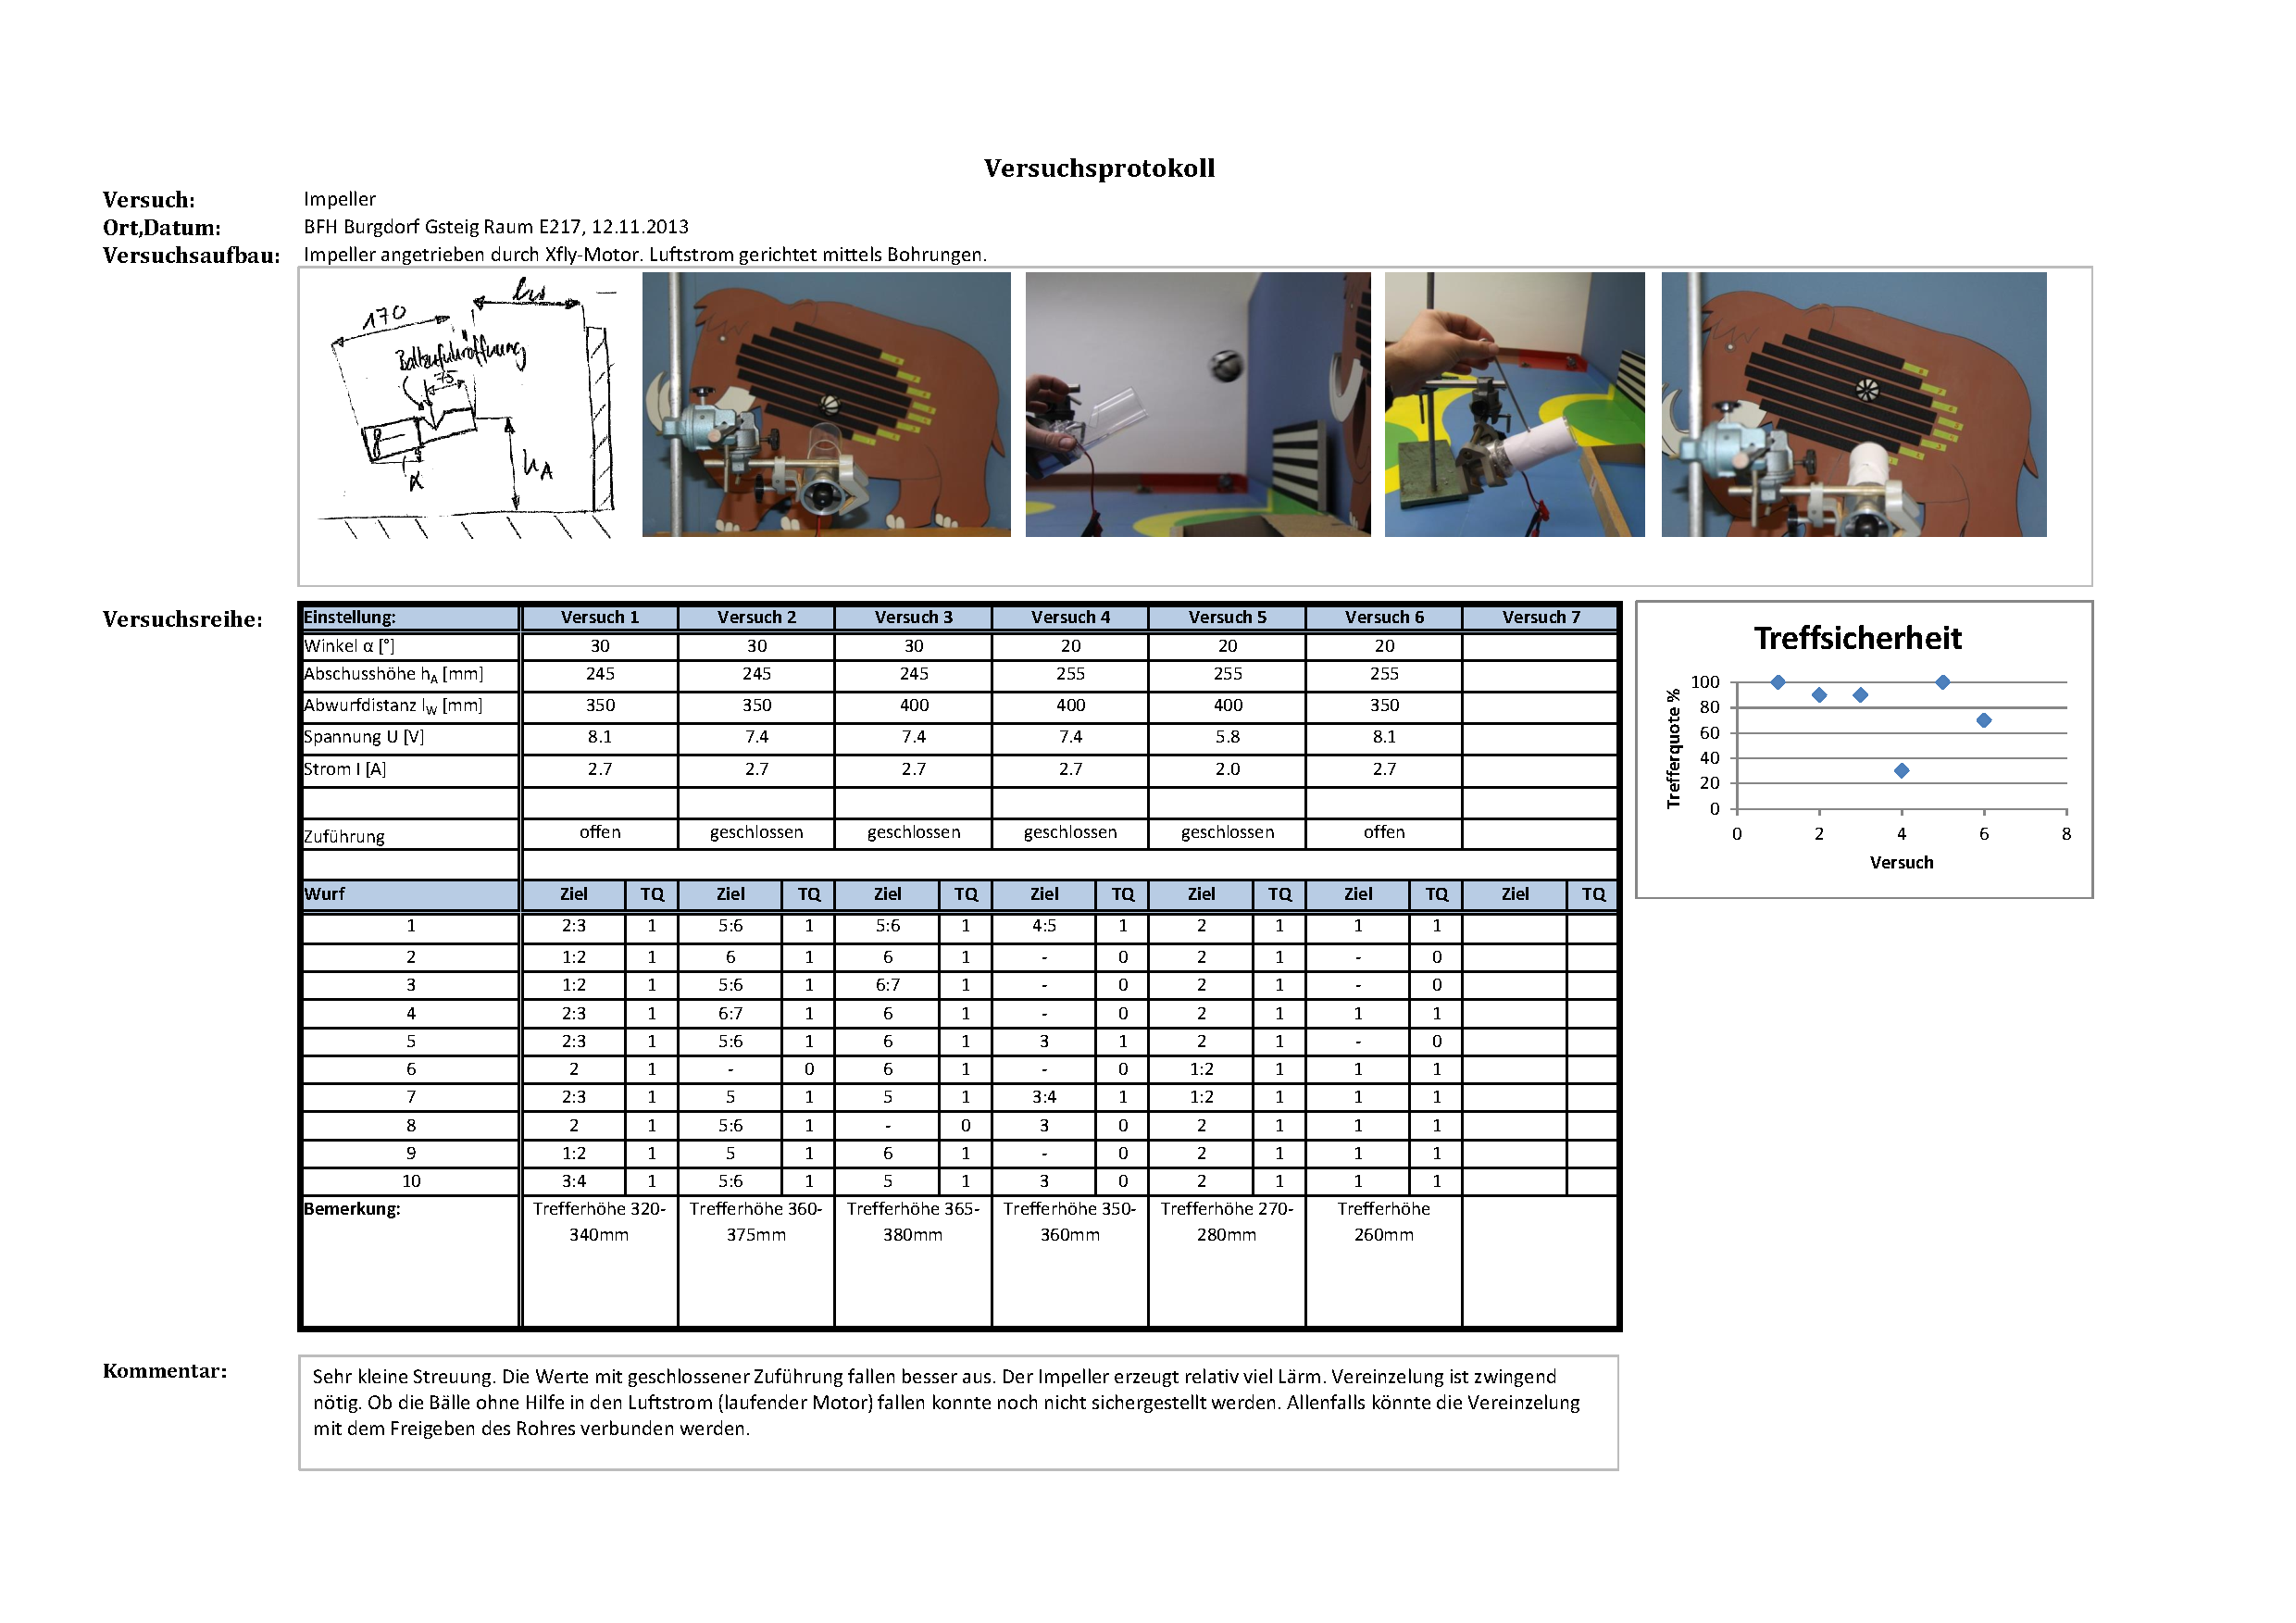
\includepdf[scale=0.80, pagecommand={}, pages=-, landscape=true]{appendix/image/d_Testprotokoll_Impeller.pdf}
    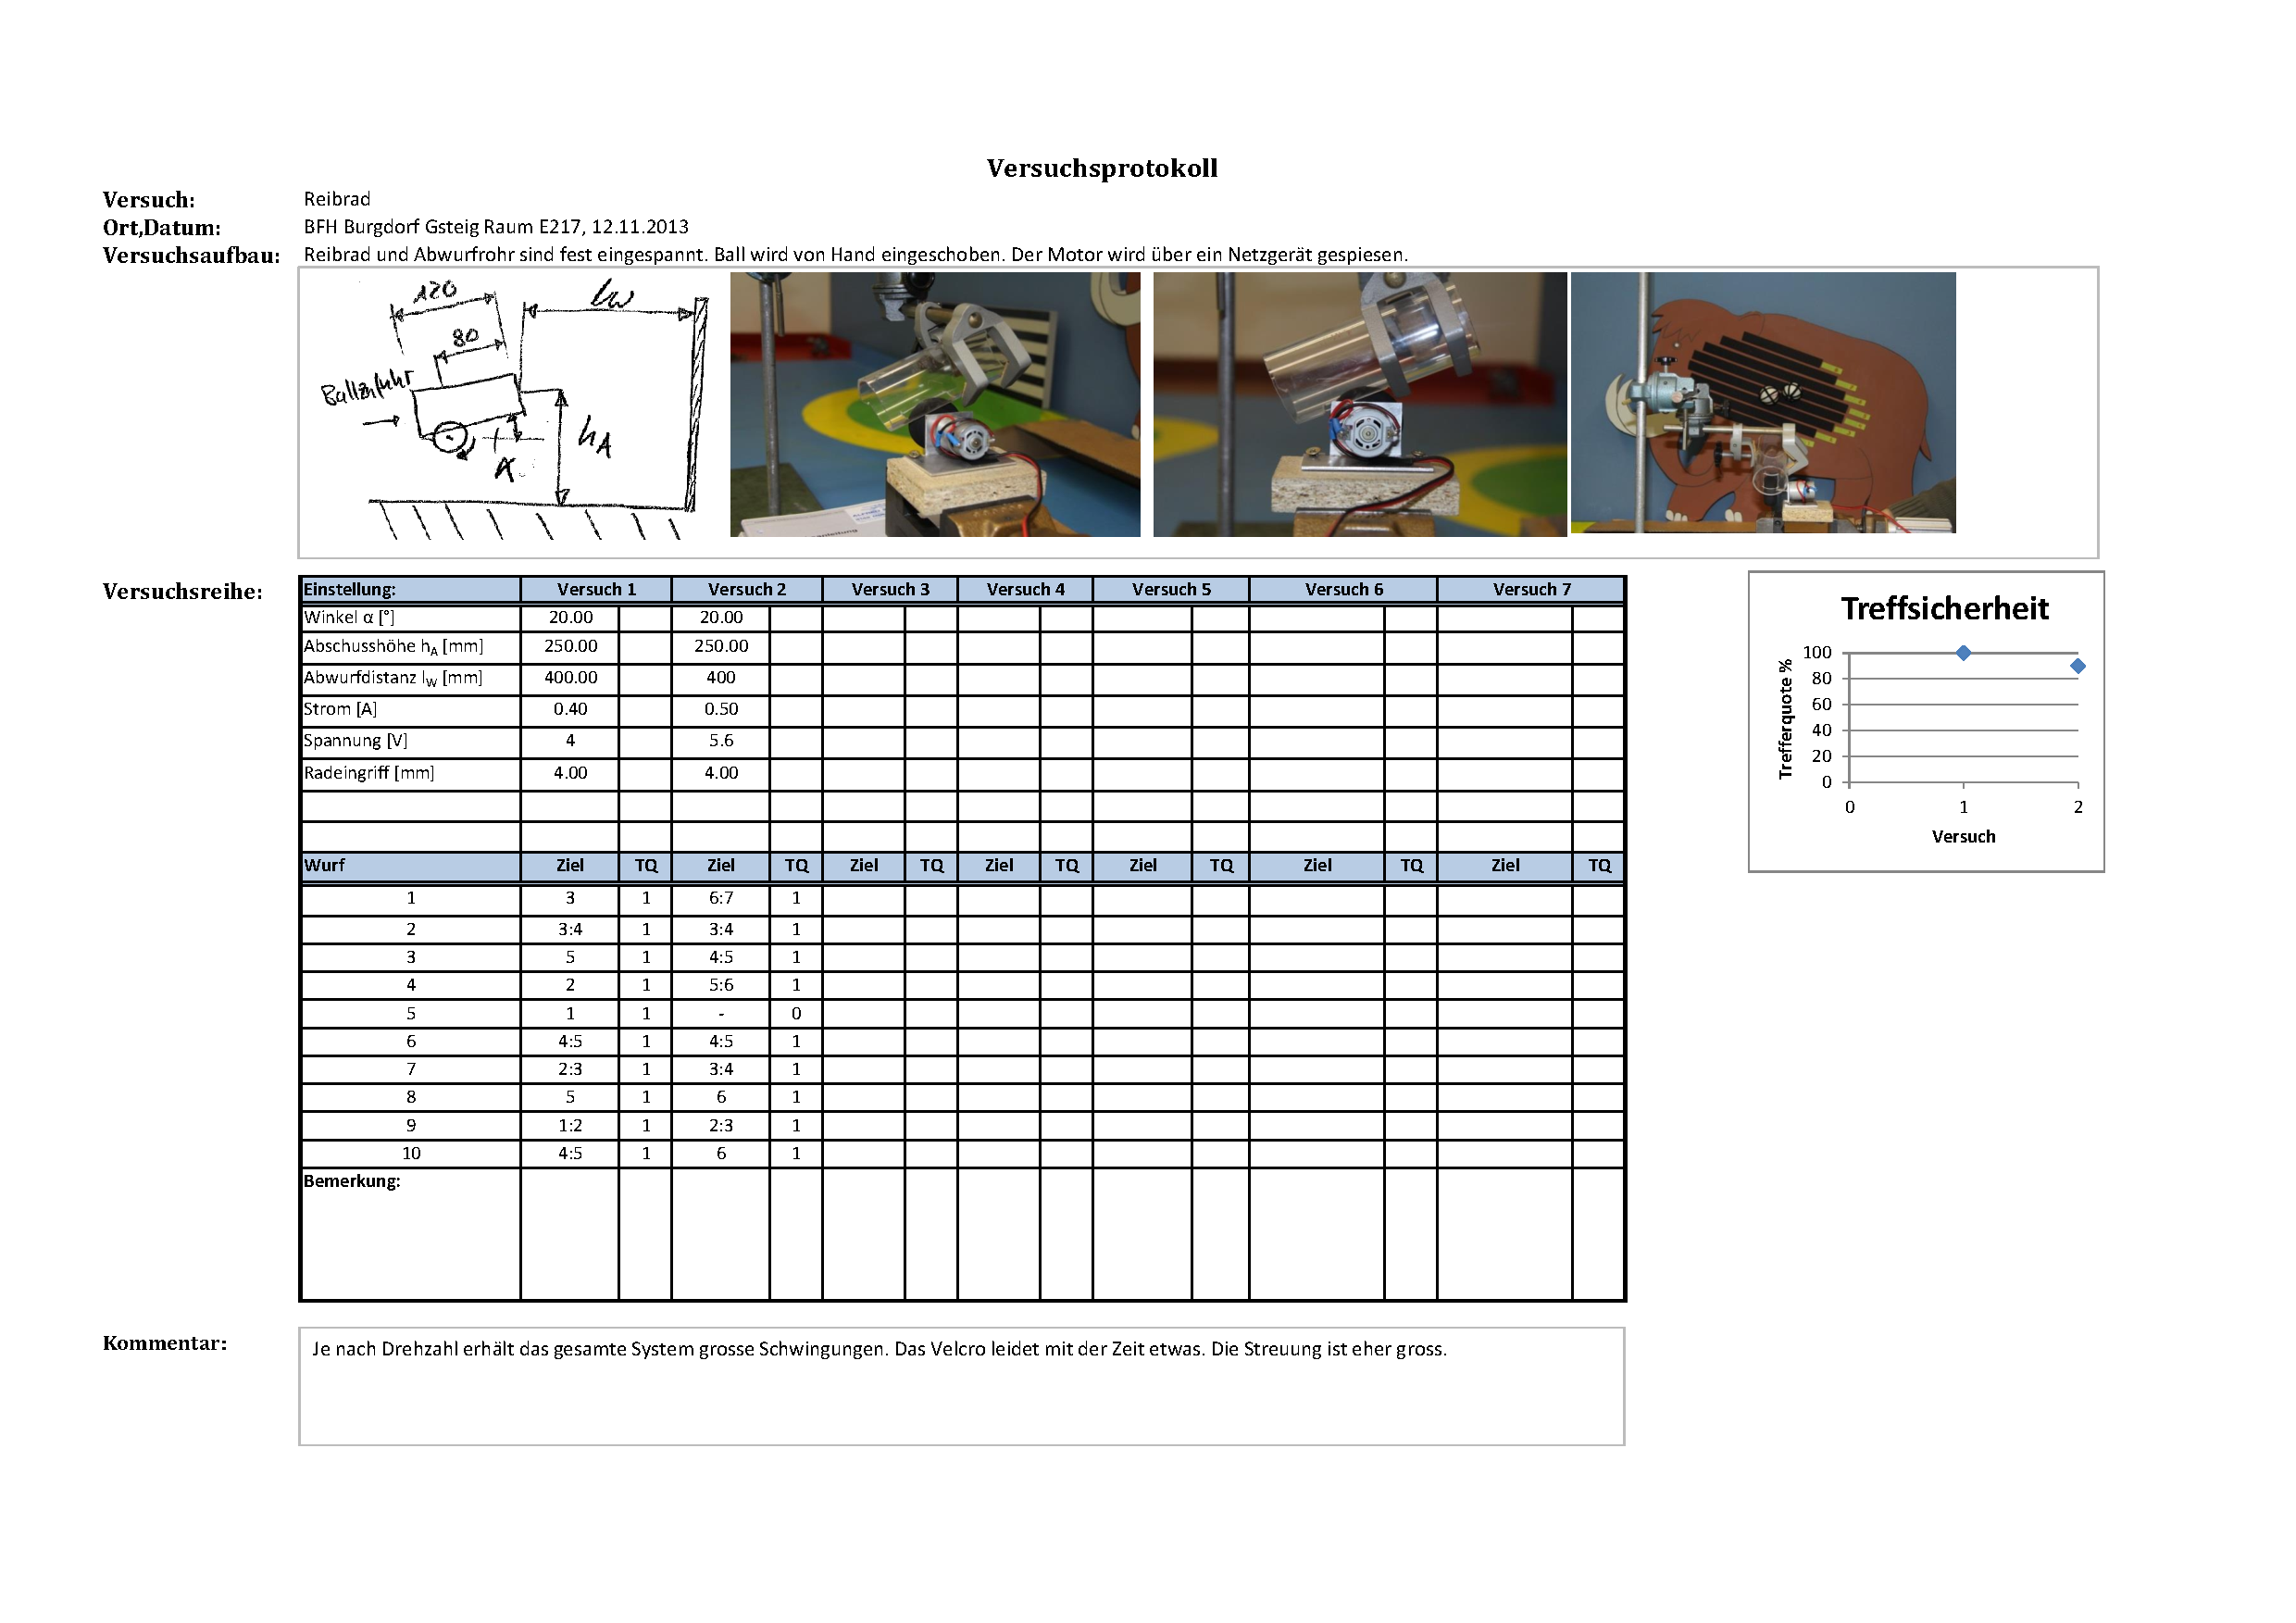
\includepdf[scale=0.80, pagecommand={}, pages=1, landscape=true]{appendix/image/d_Testprotokoll_Reibrad.pdf}
    %
    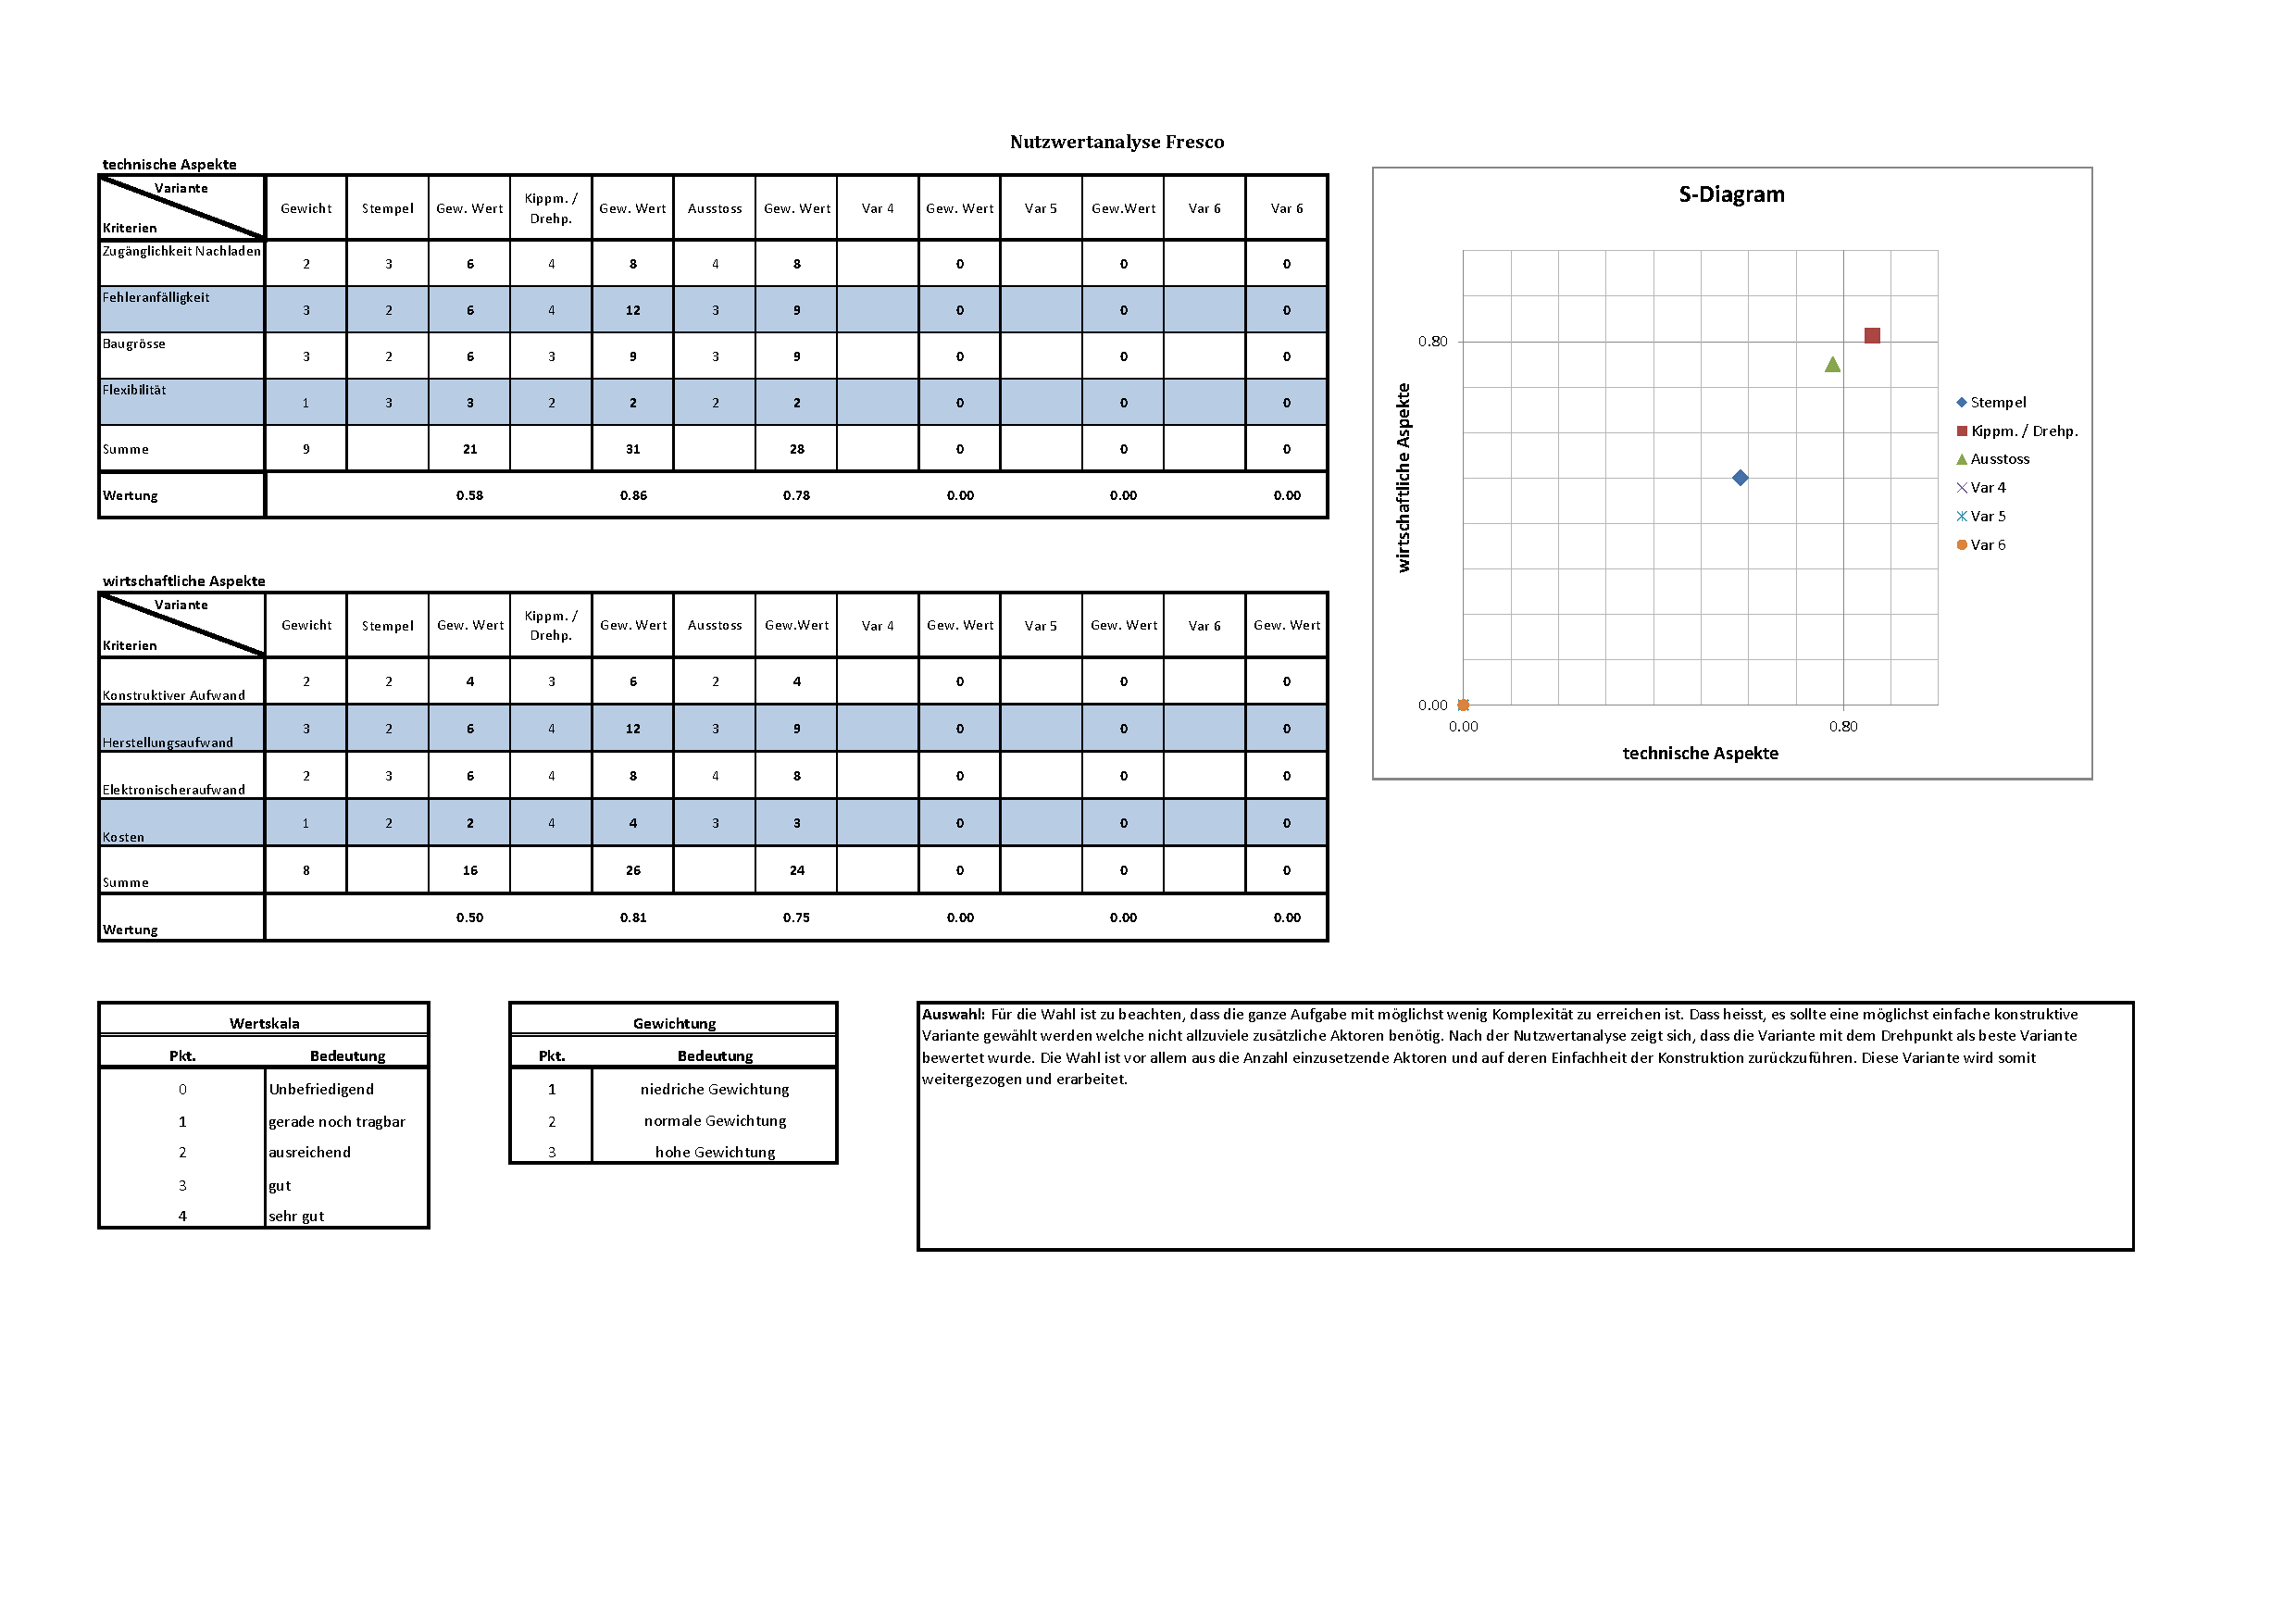
\includepdf[scale=0.80, pagecommand={}, pages=-, landscape=true]{appendix/image/d_S-Diagramm_Fresco.pdf}
    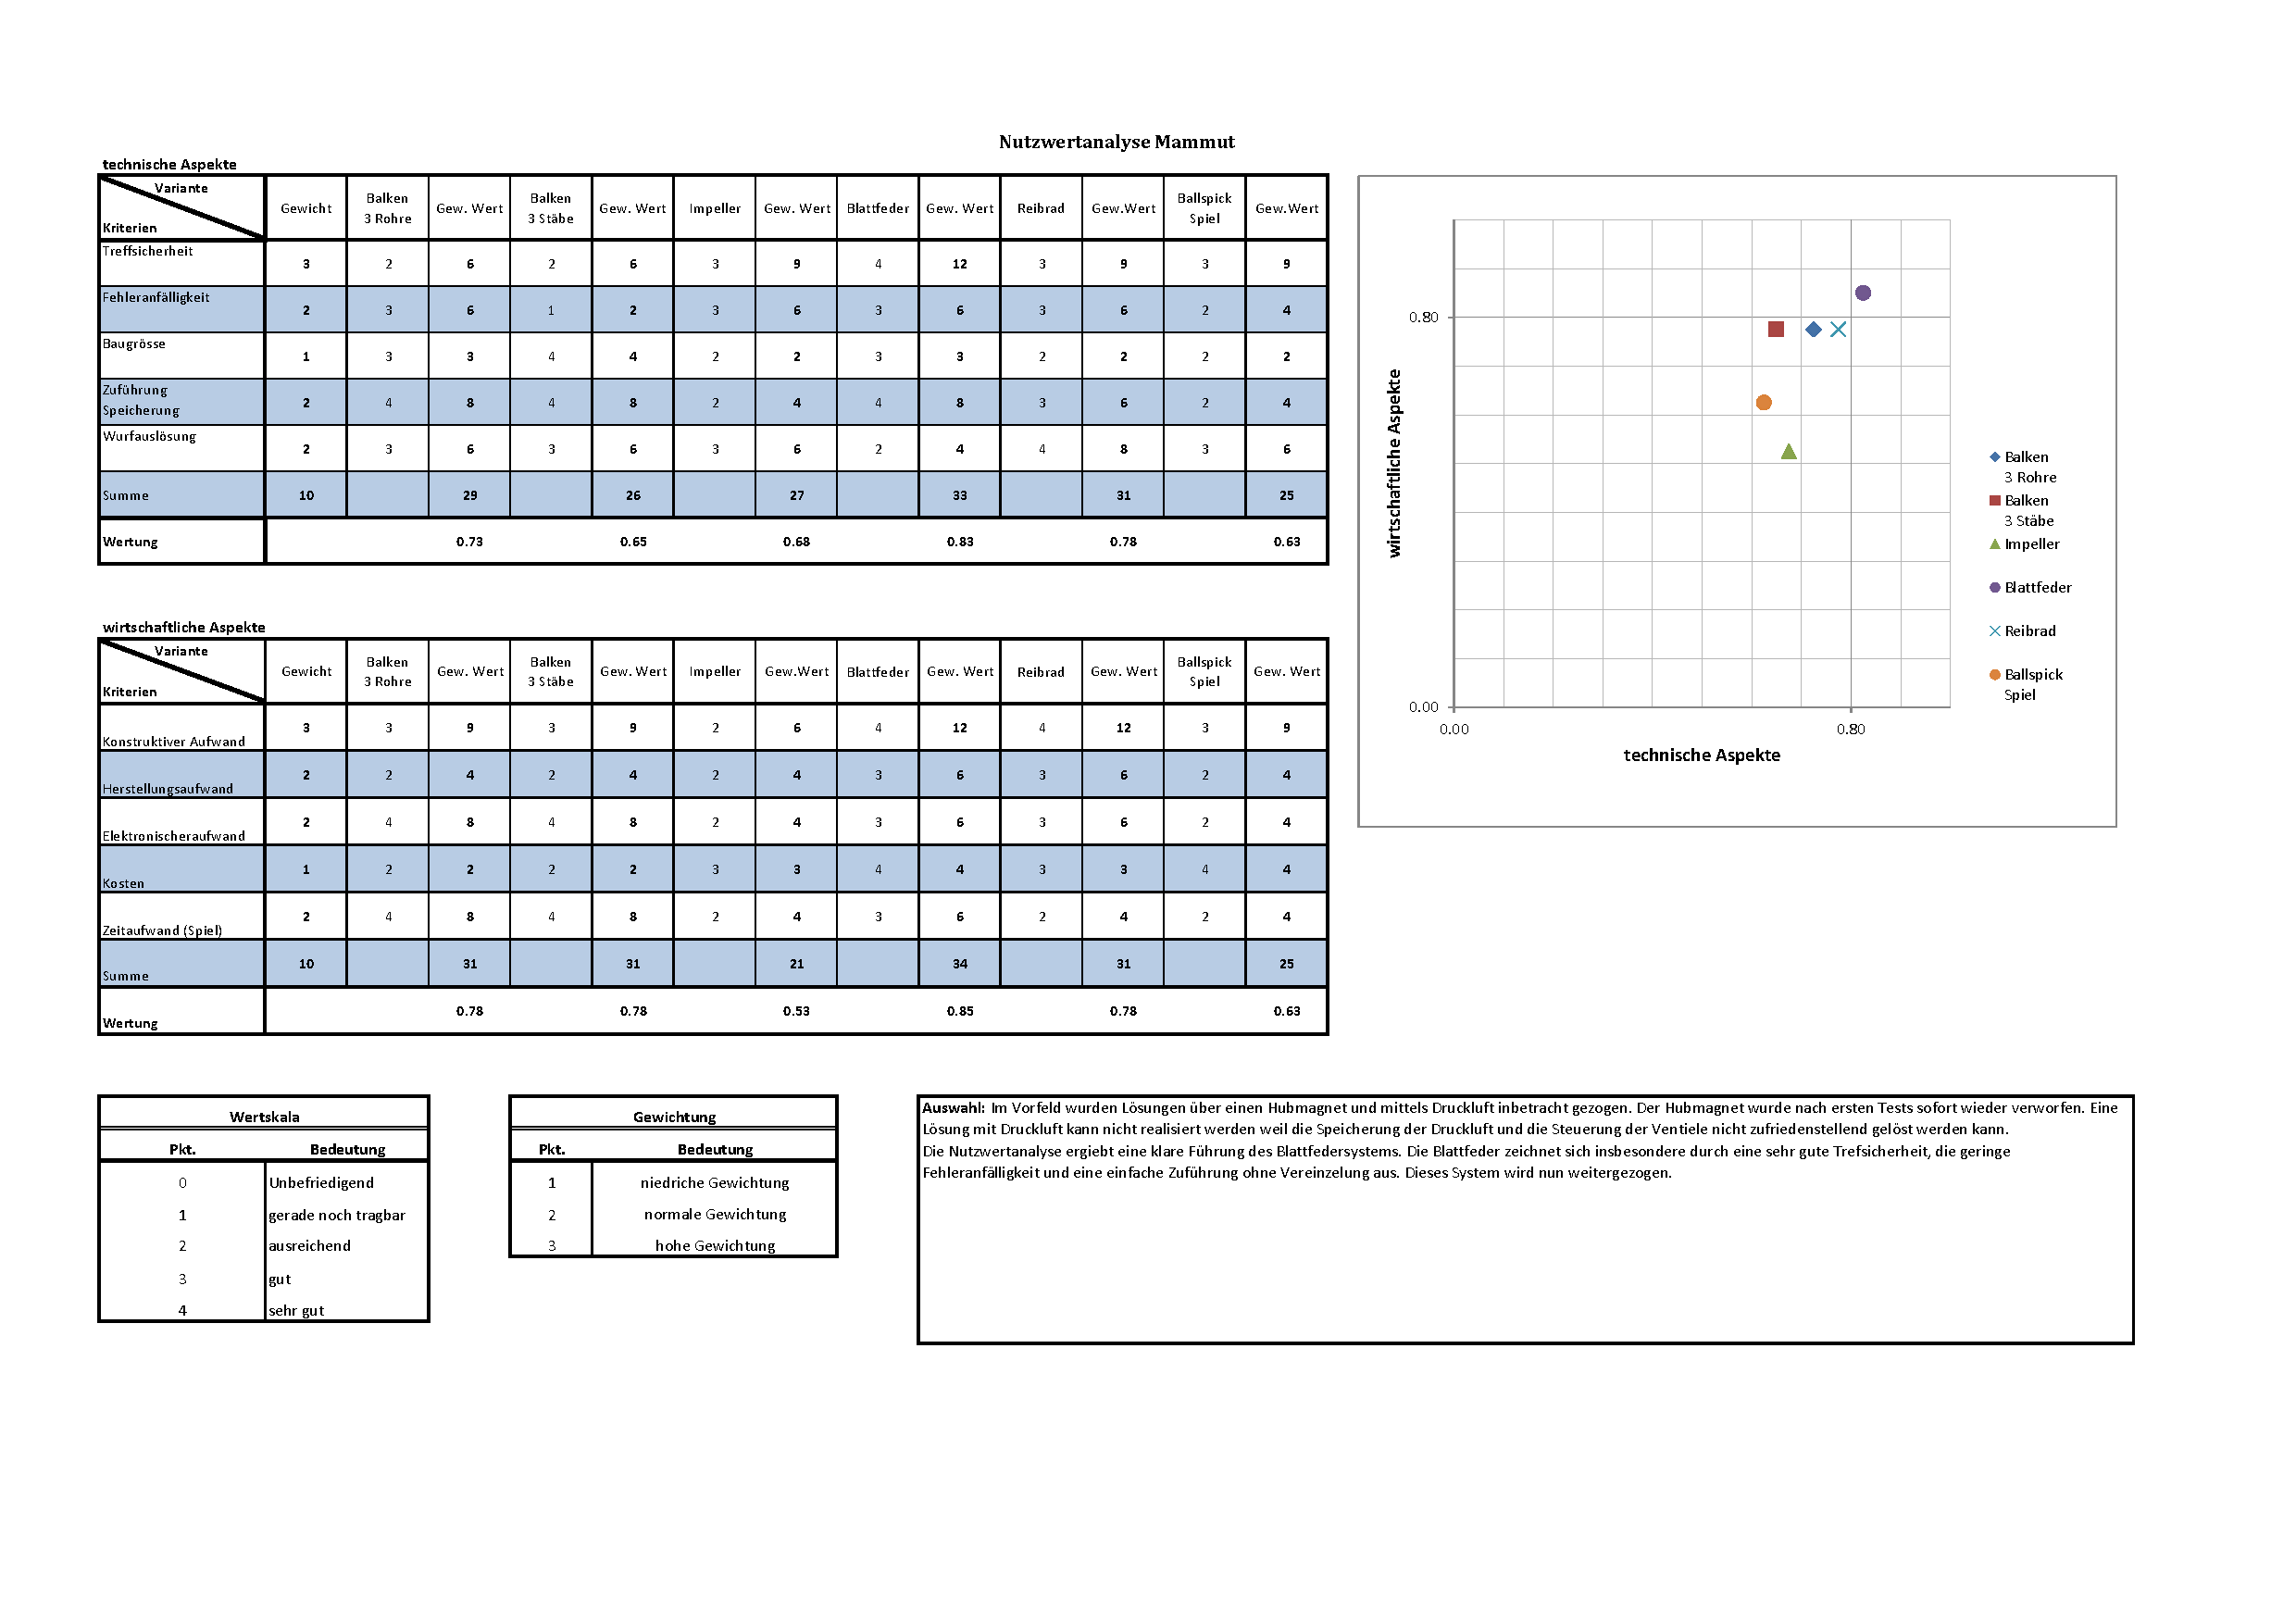
\includepdf[scale=0.80, pagecommand={}, pages=-, landscape=true]{appendix/image/d_S-Diagramm_Mammout.pdf}
    %
    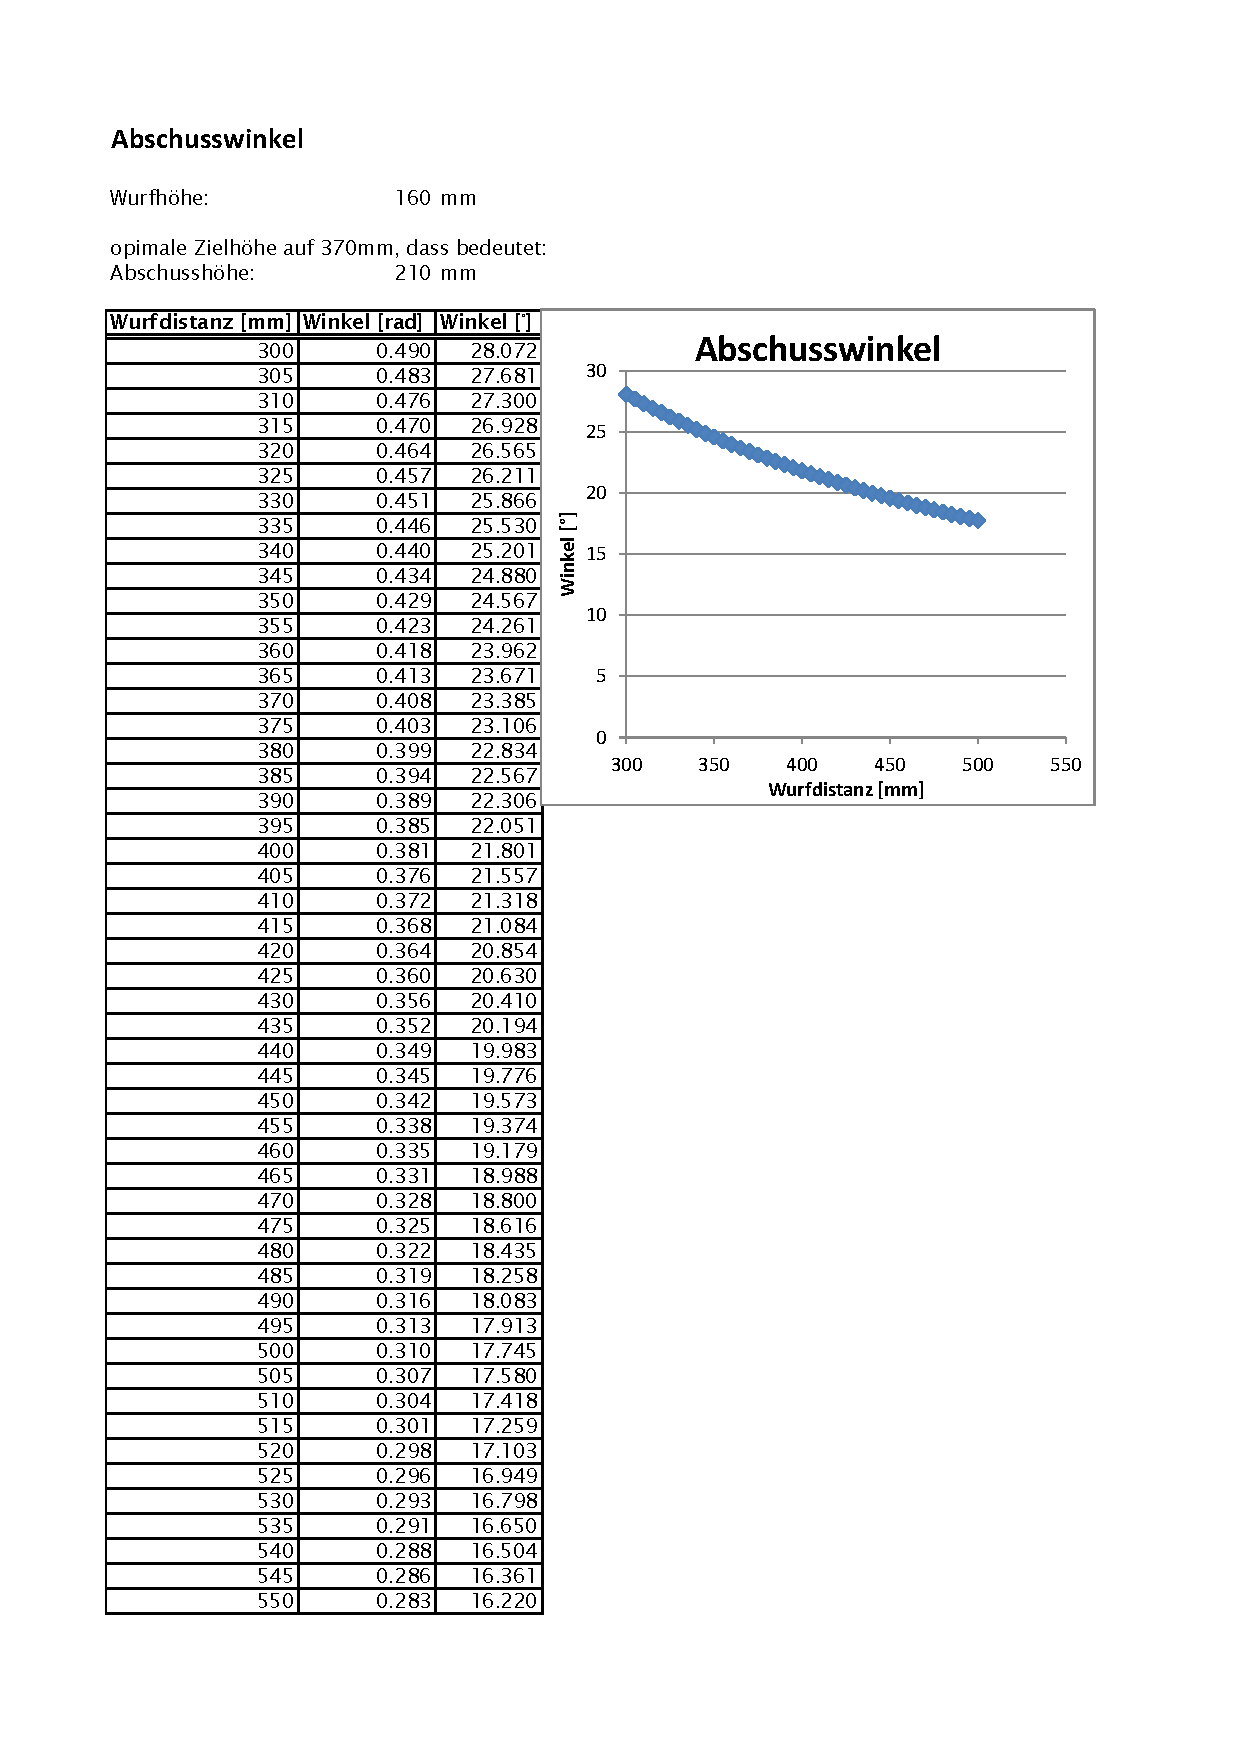
\includepdf[scale=0.85, pagecommand={}, pages=-]{appendix/image/d_Abschusswinkel_Berechnung.pdf}
    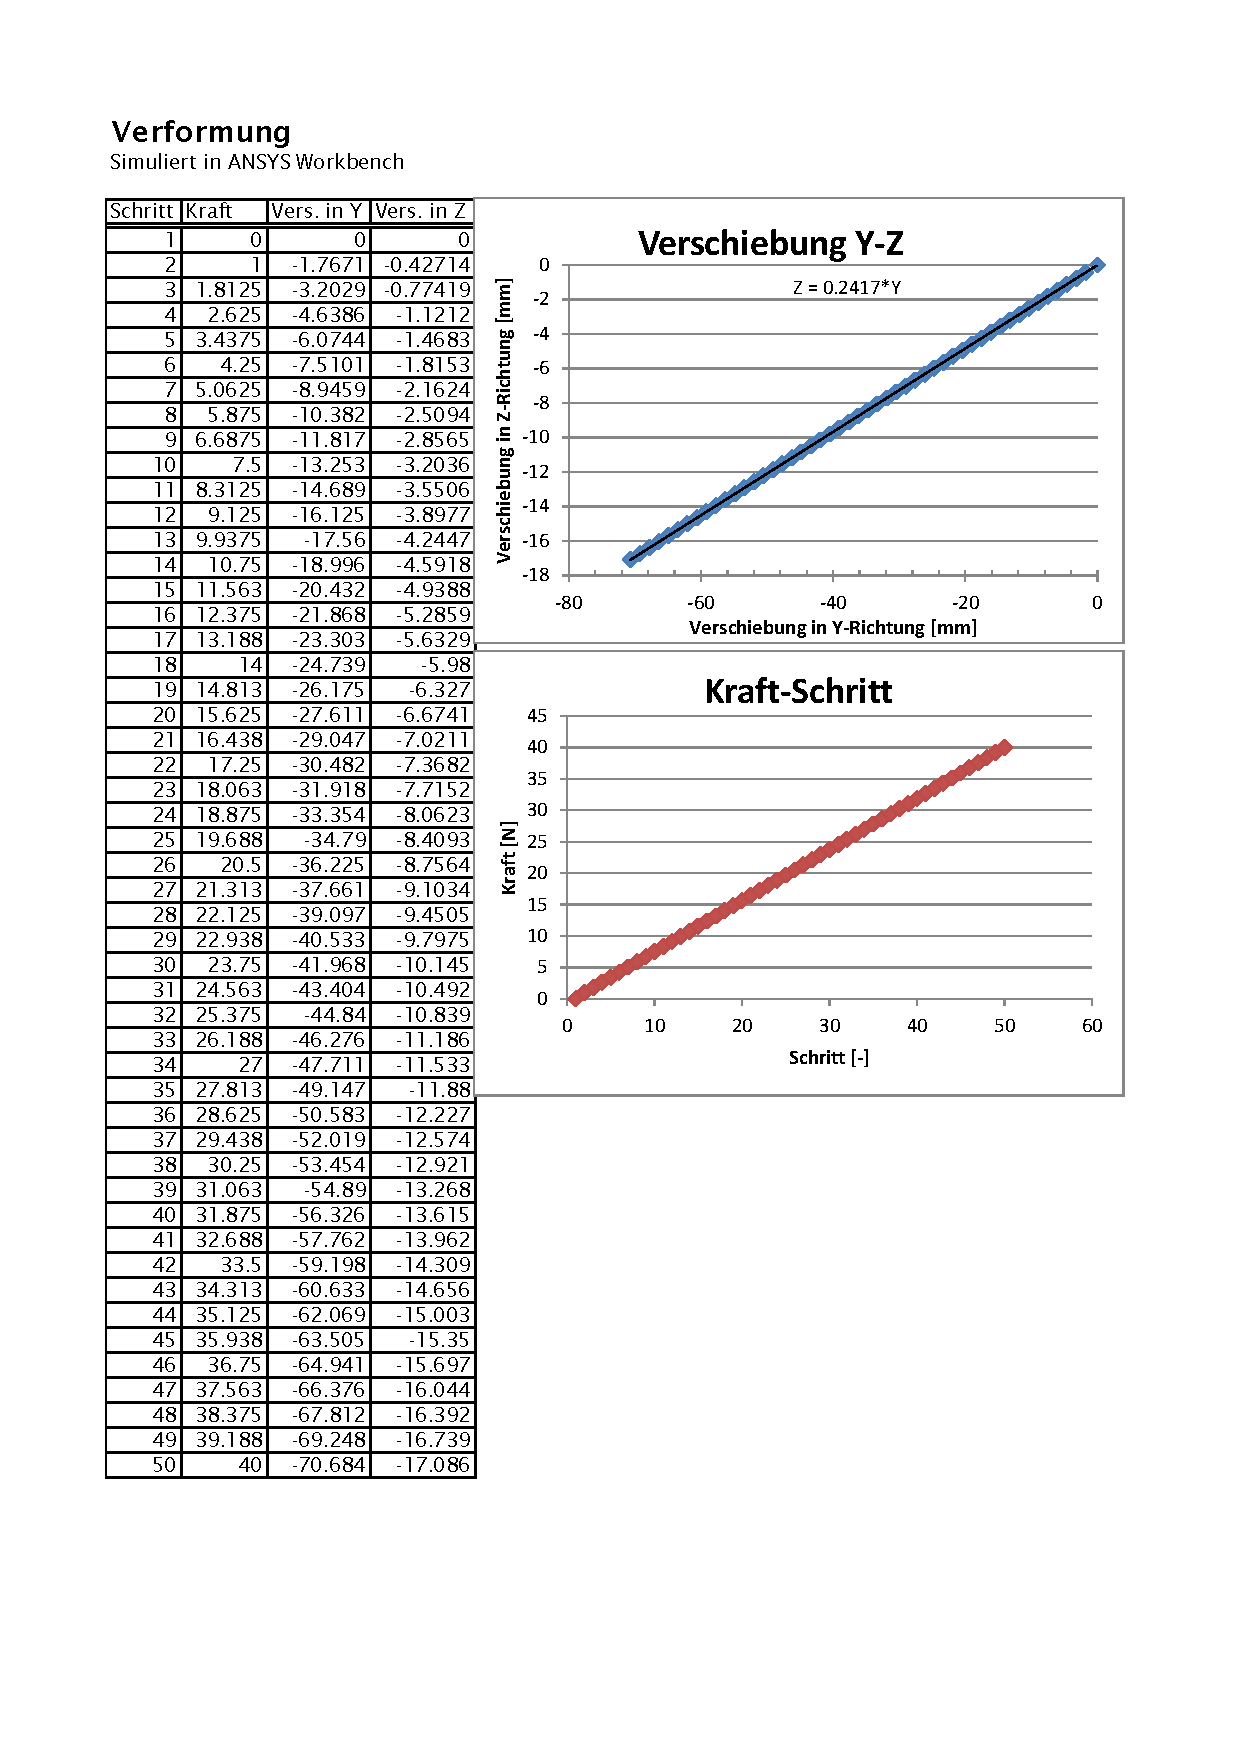
\includepdf[scale=0.85, pagecommand={}, pages=-]{appendix/image/d_Verformung_Blattfeder_Messdaten.pdf}
    %
\includepdf[scale=0.85,pagecommand={\thispagestyle{plain}}, pages=-]{appendix/image/b_pflichtenheft.pdf}
    %
%PA2
	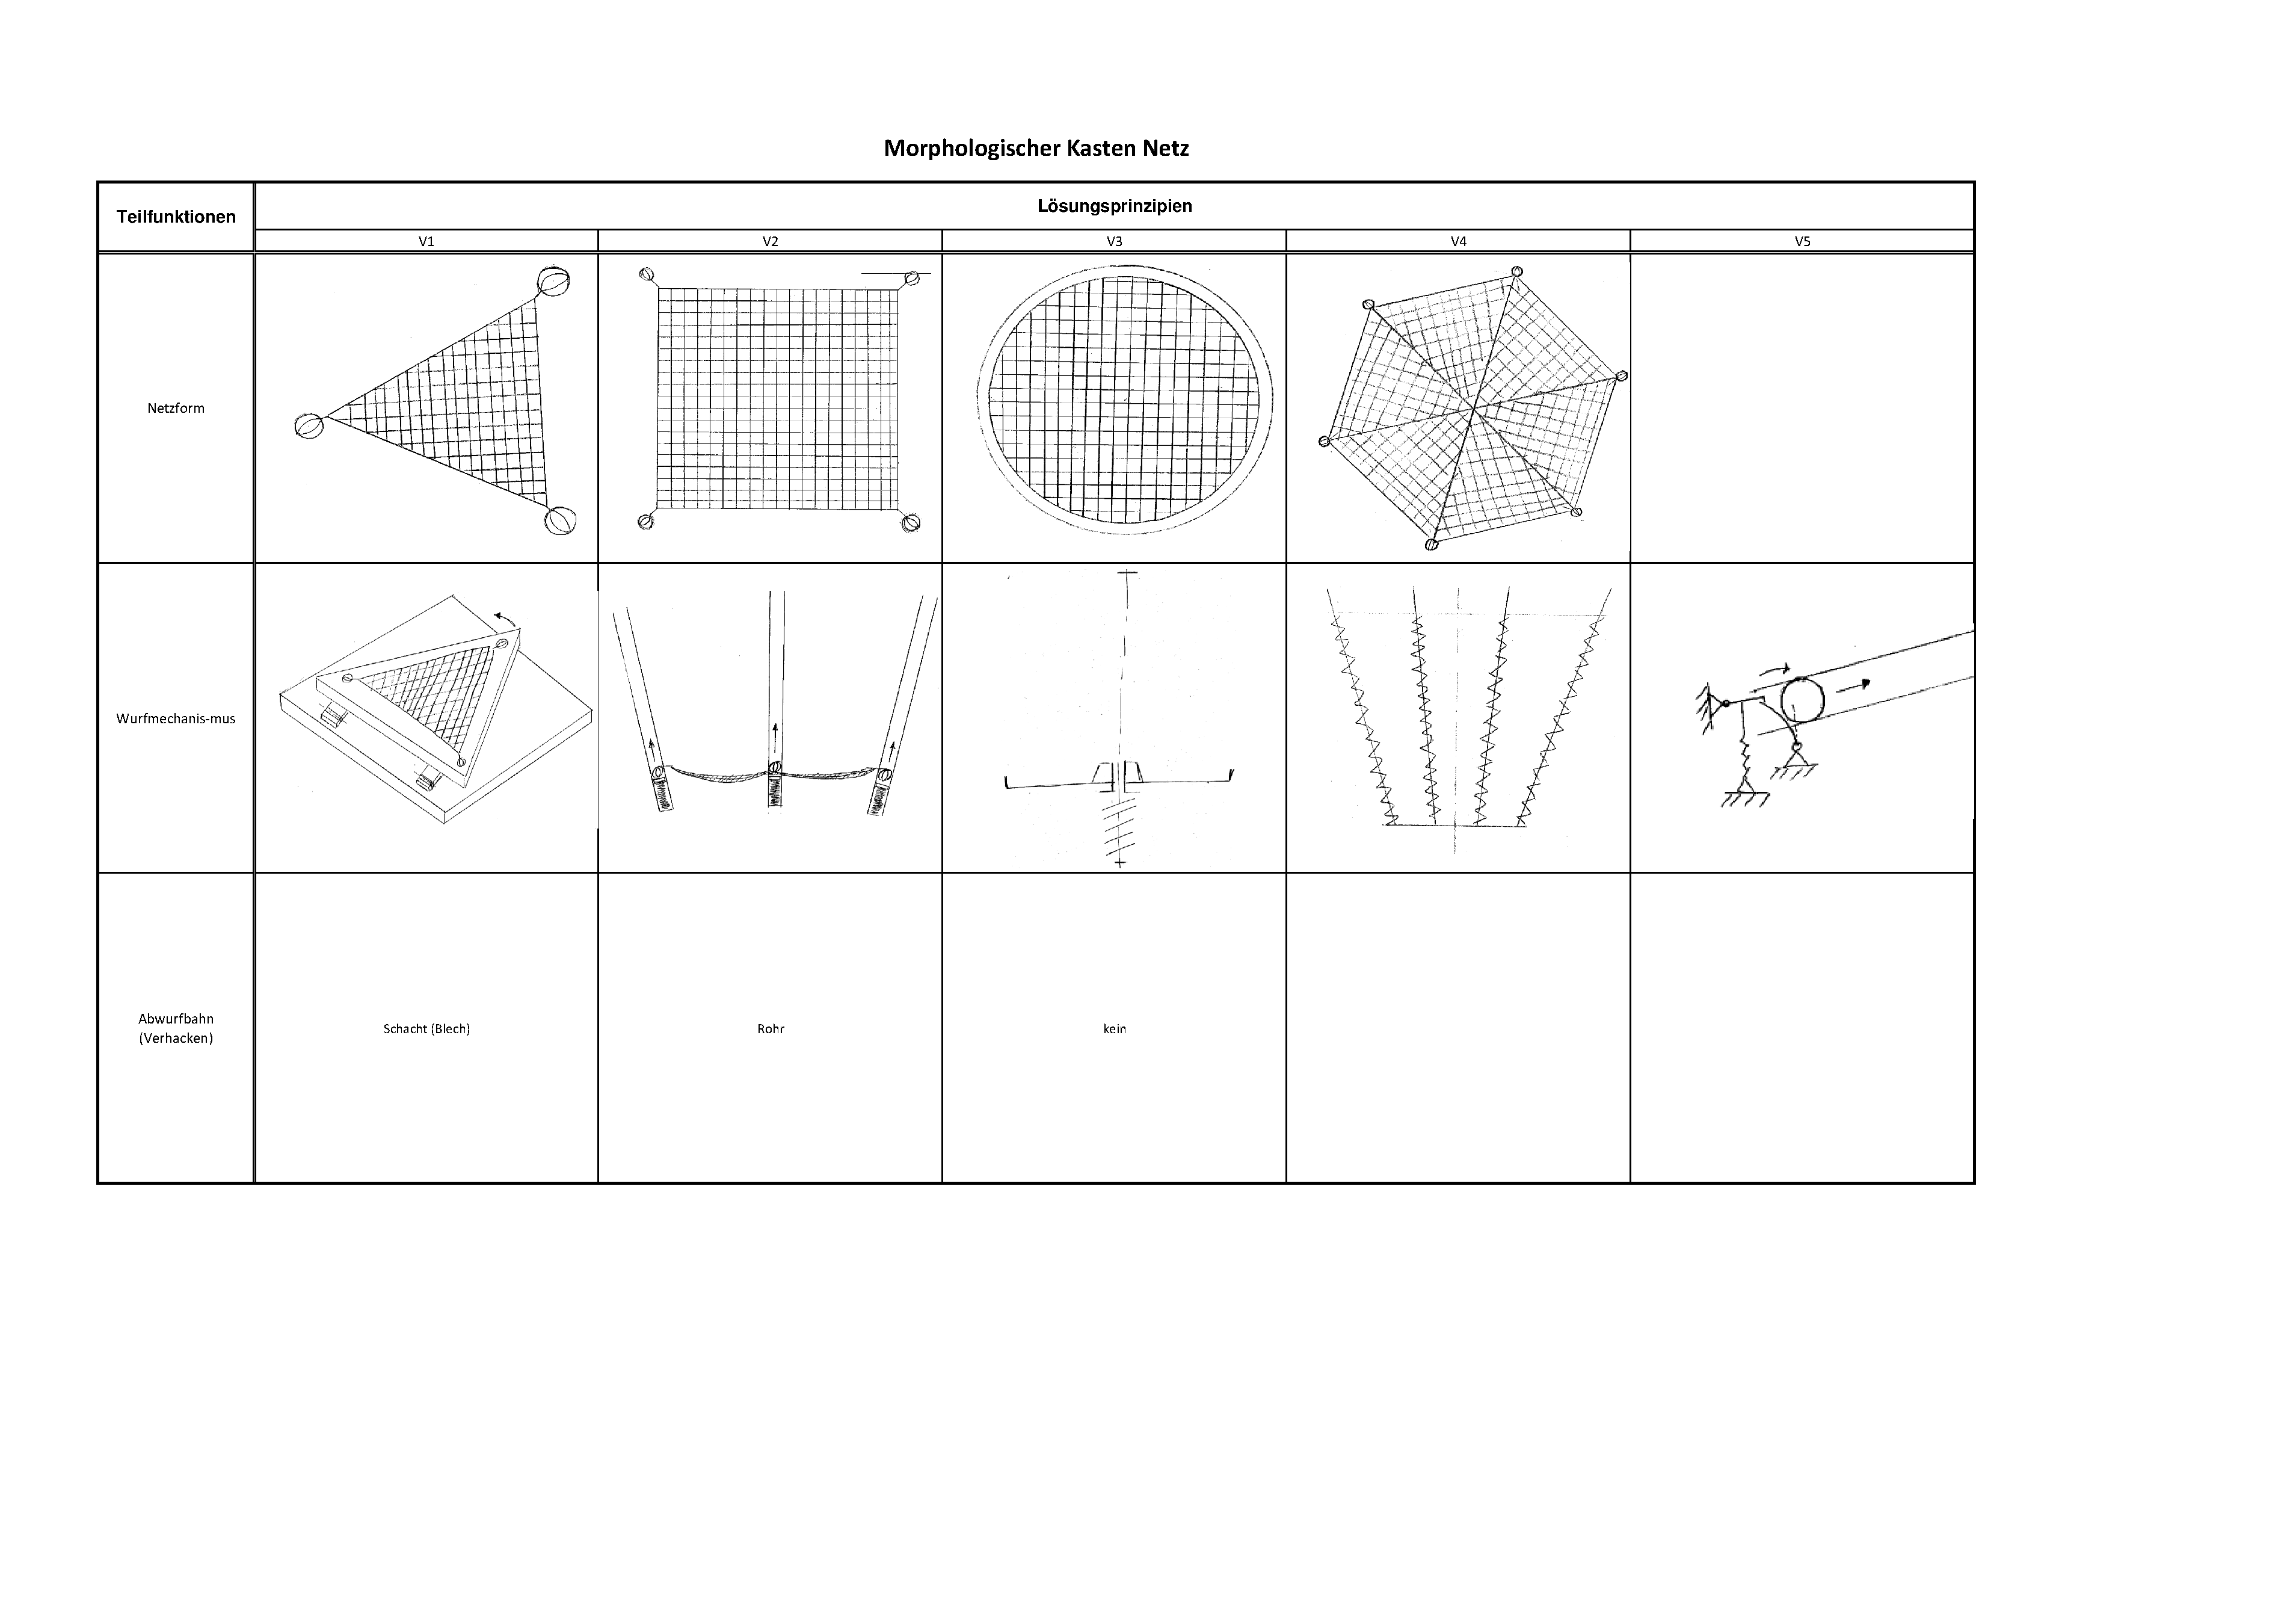
\includepdf[scale=0.80, pagecommand={}, pages=-, landscape=true]{appendix/Anhang_Mechanik_PA2/Konzept-_Ausarbeitungphase_mech/1Morph_Kast_Netz.pdf}
    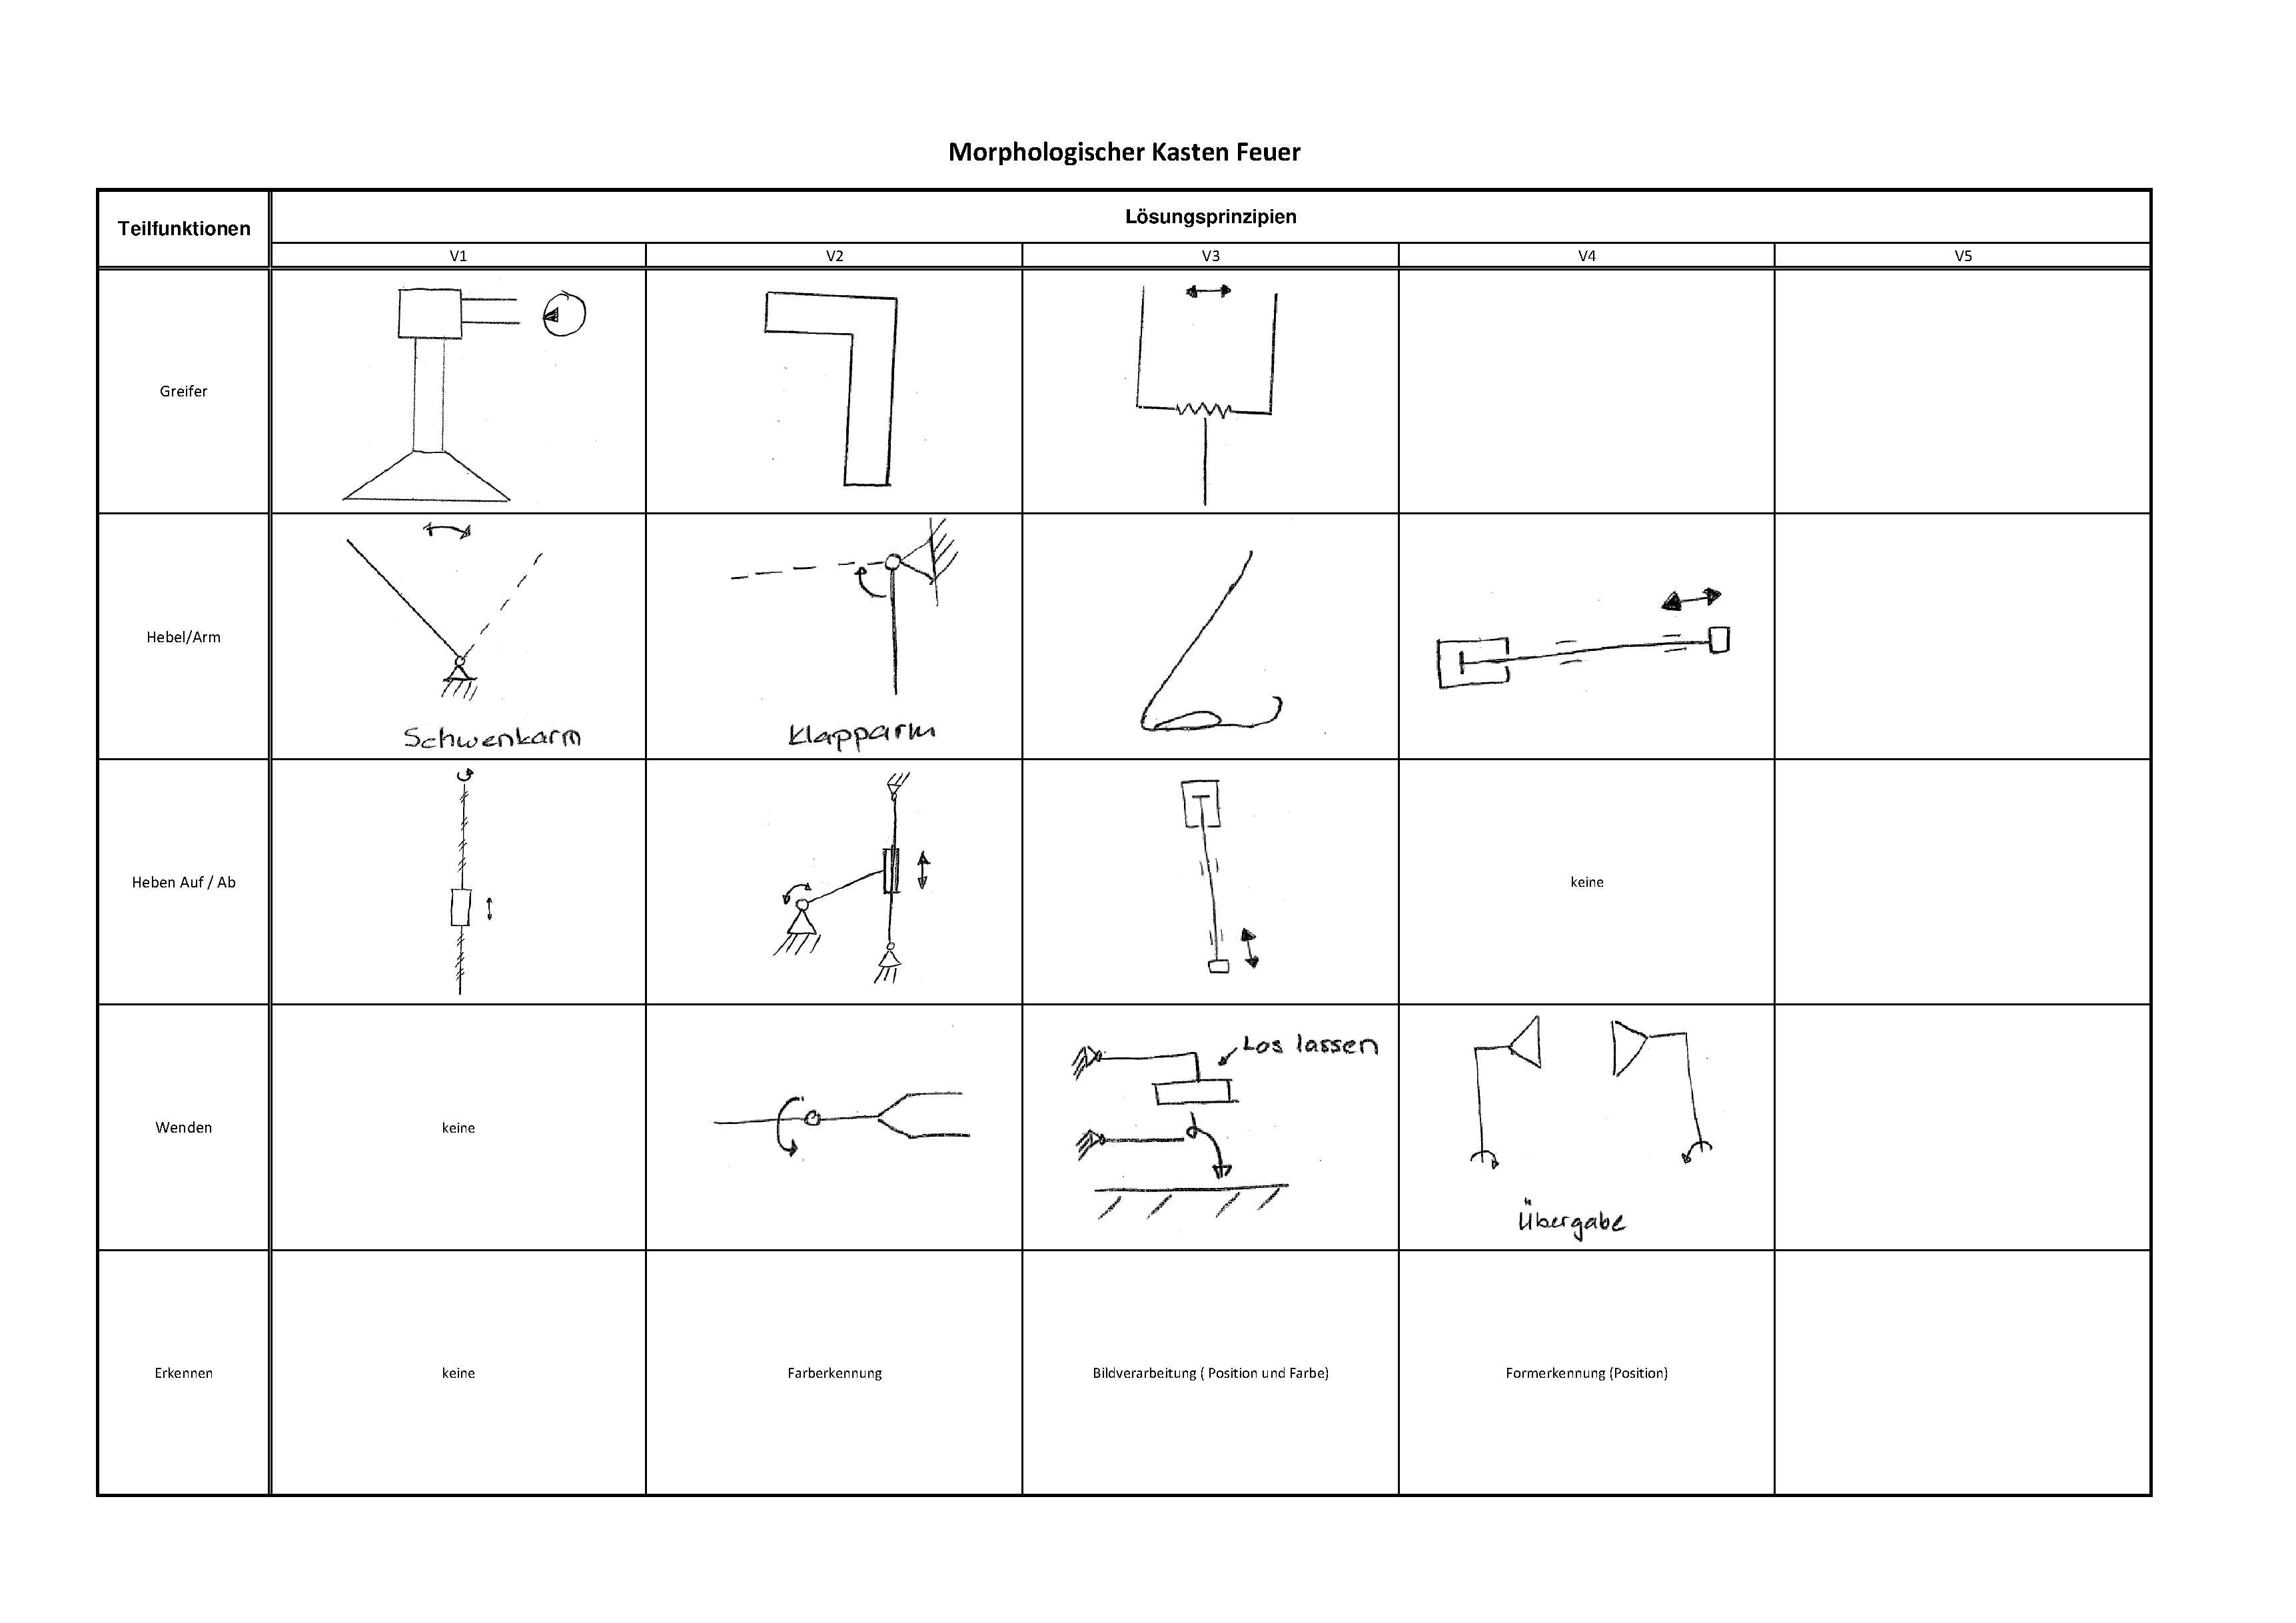
\includepdf[scale=0.80, pagecommand={}, pages=-, landscape=true]{appendix/Anhang_Mechanik_PA2/Konzept-_Ausarbeitungphase_mech/2Morph_Kast_Feuer.pdf}
    %
   	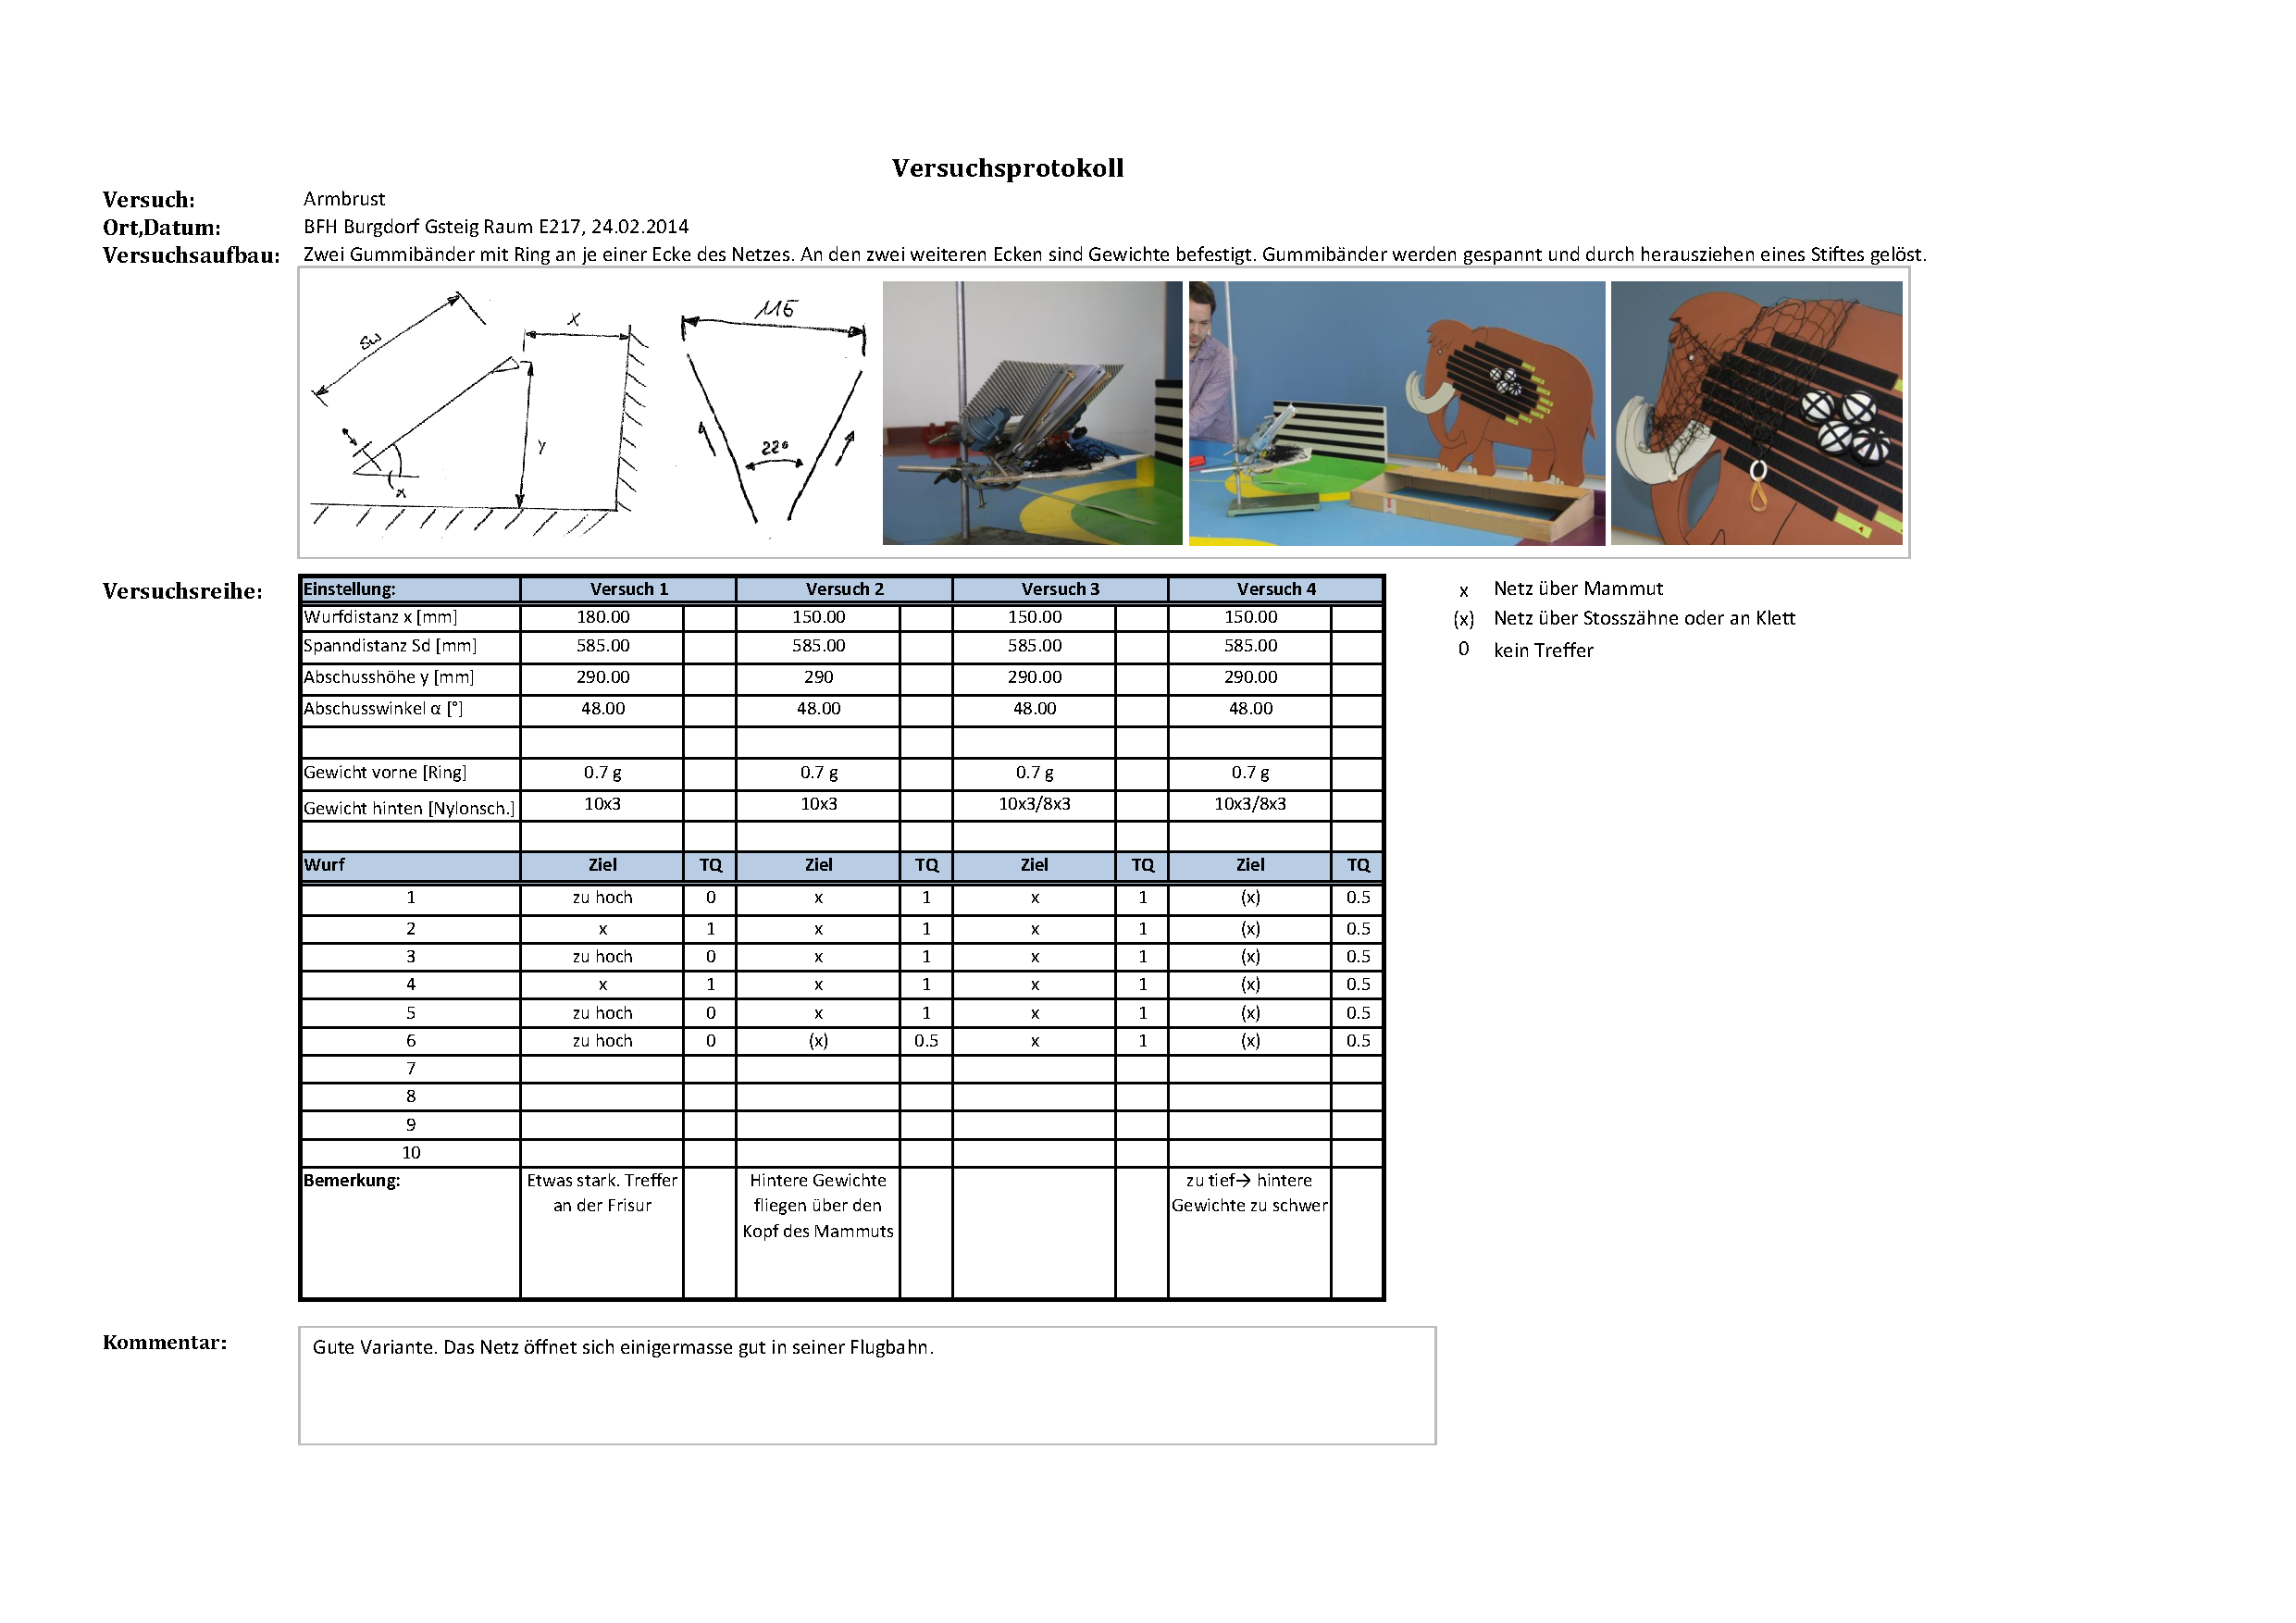
\includepdf[scale=0.80, pagecommand={}, pages=-, landscape=true]{appendix/Anhang_Mechanik_PA2/Konzept-_Ausarbeitungphase_mech/3Testprotokoll_Netz_Armbrust.pdf}
    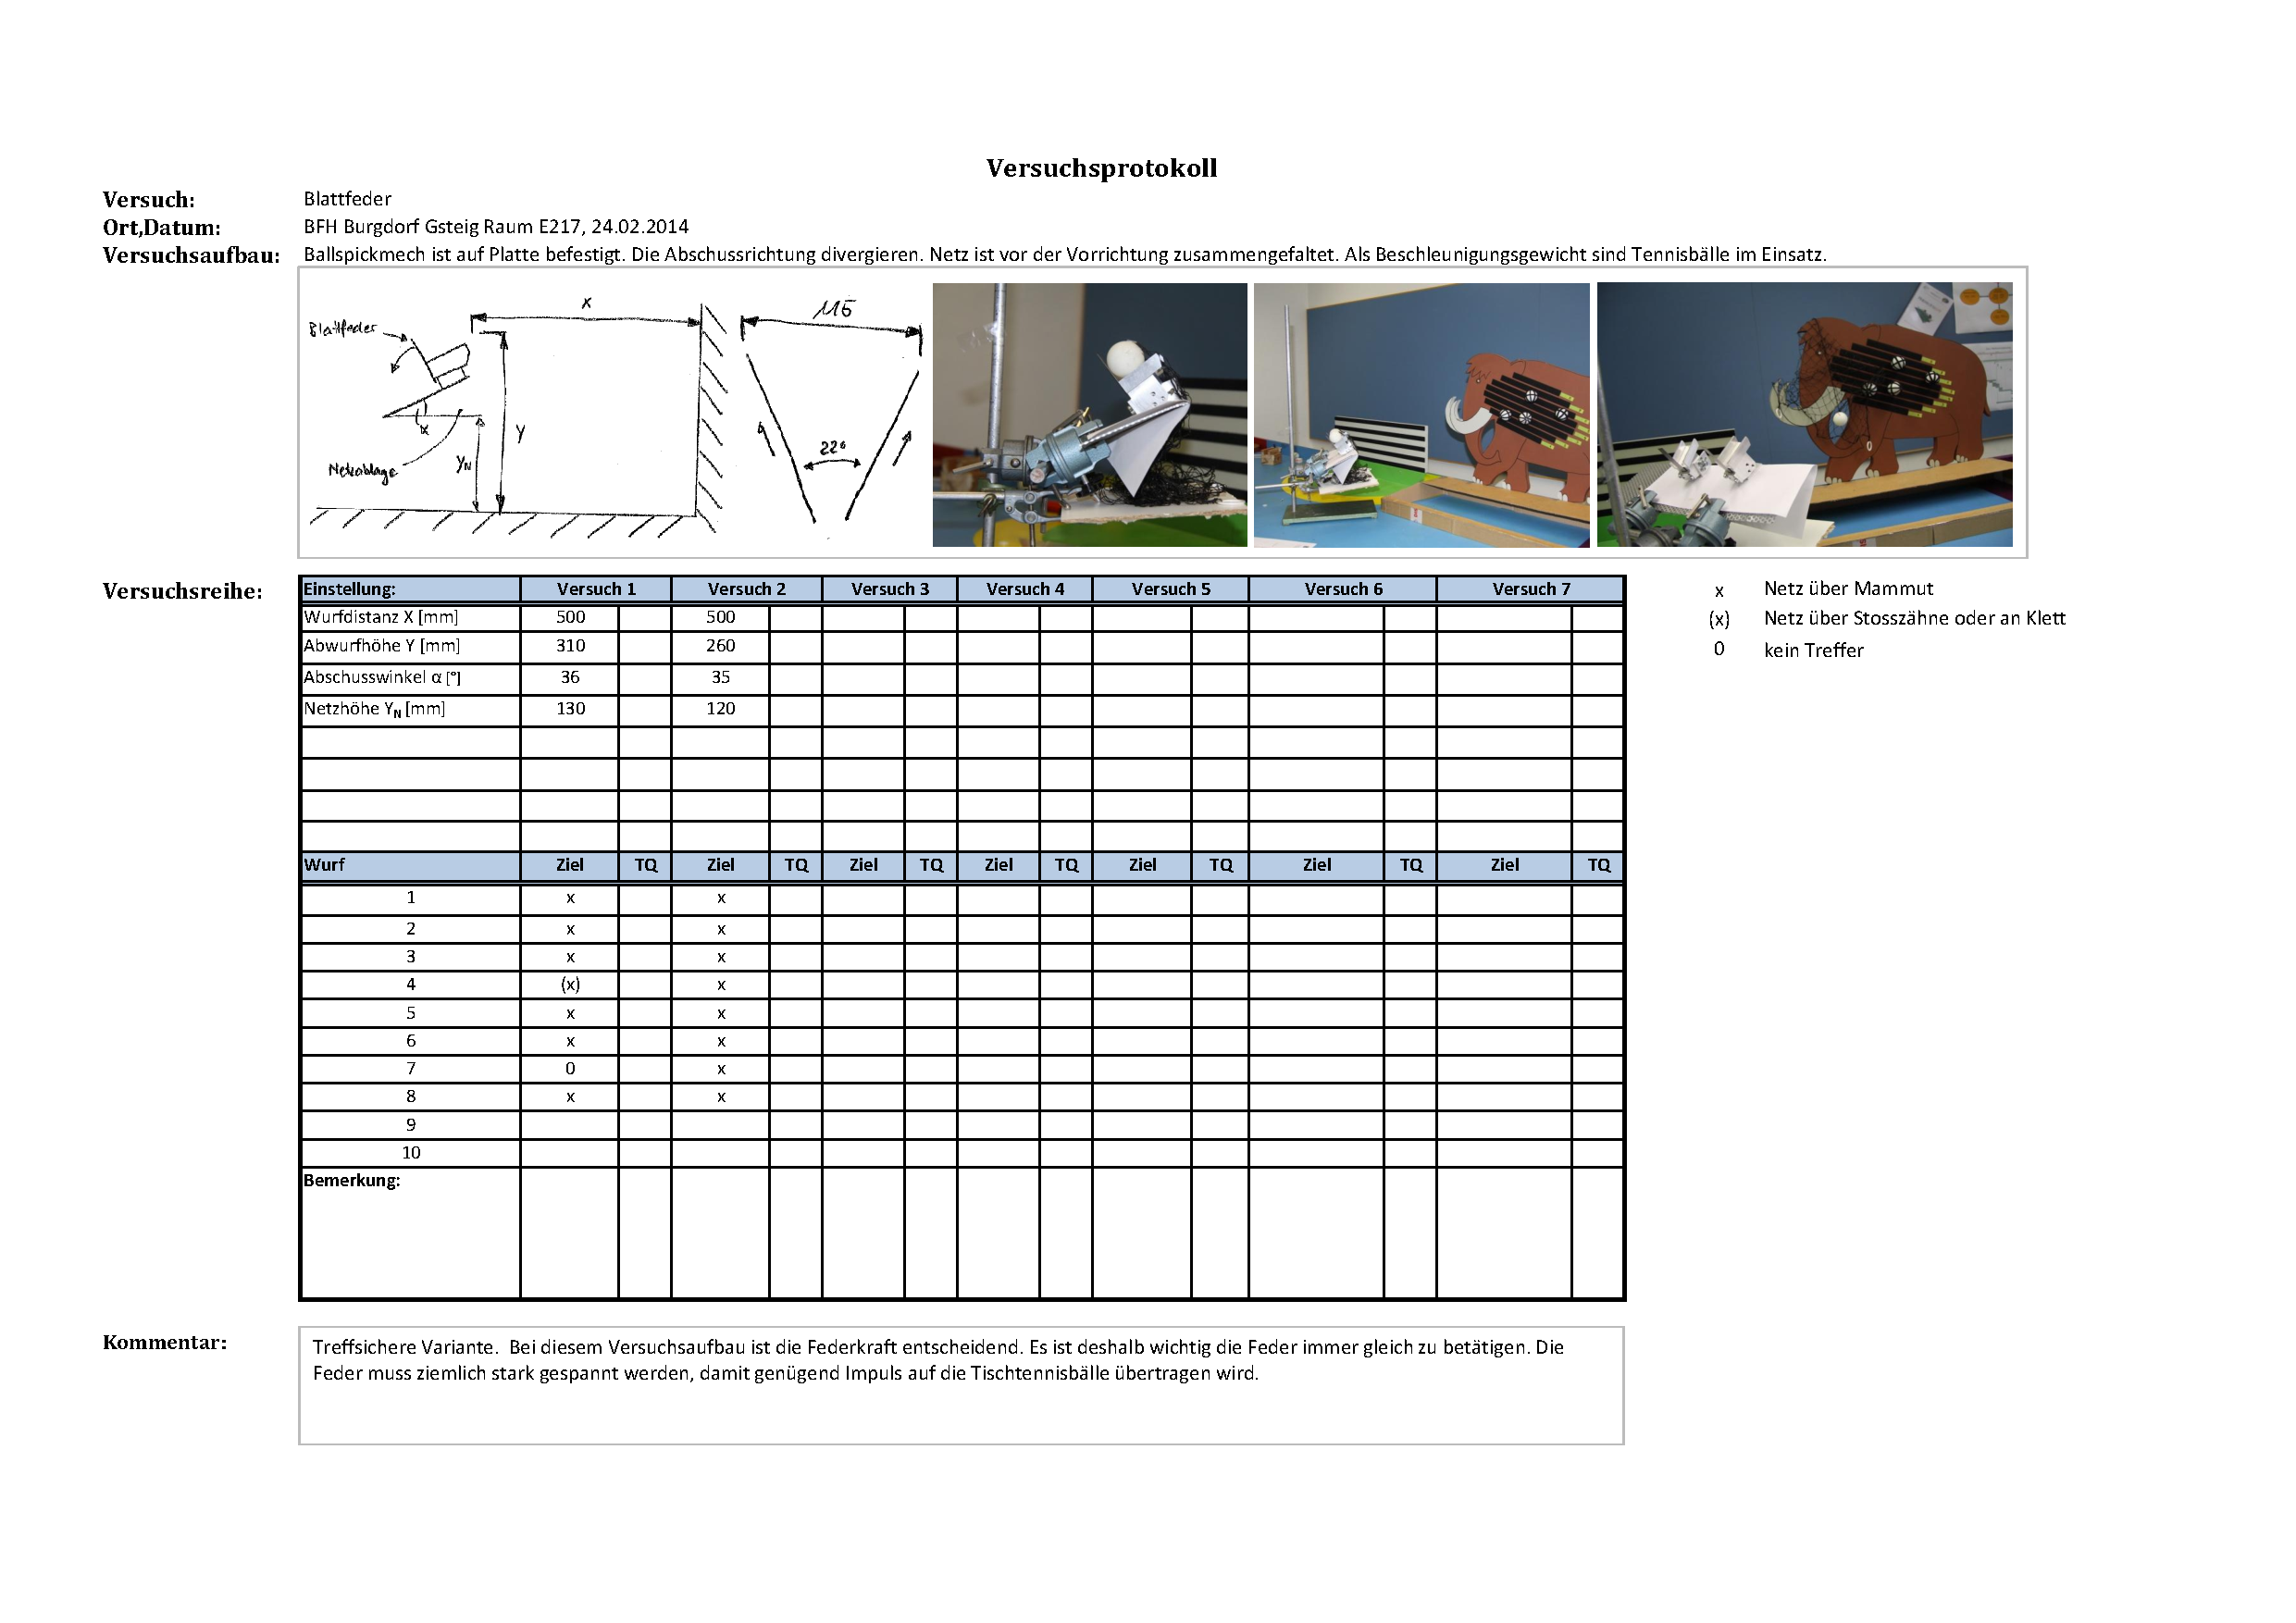
\includepdf[scale=0.80, pagecommand={}, pages=-, landscape=true]{appendix/Anhang_Mechanik_PA2/Konzept-_Ausarbeitungphase_mech/4Testprotokoll_Netz_Blattfeder.pdf}
    %
   	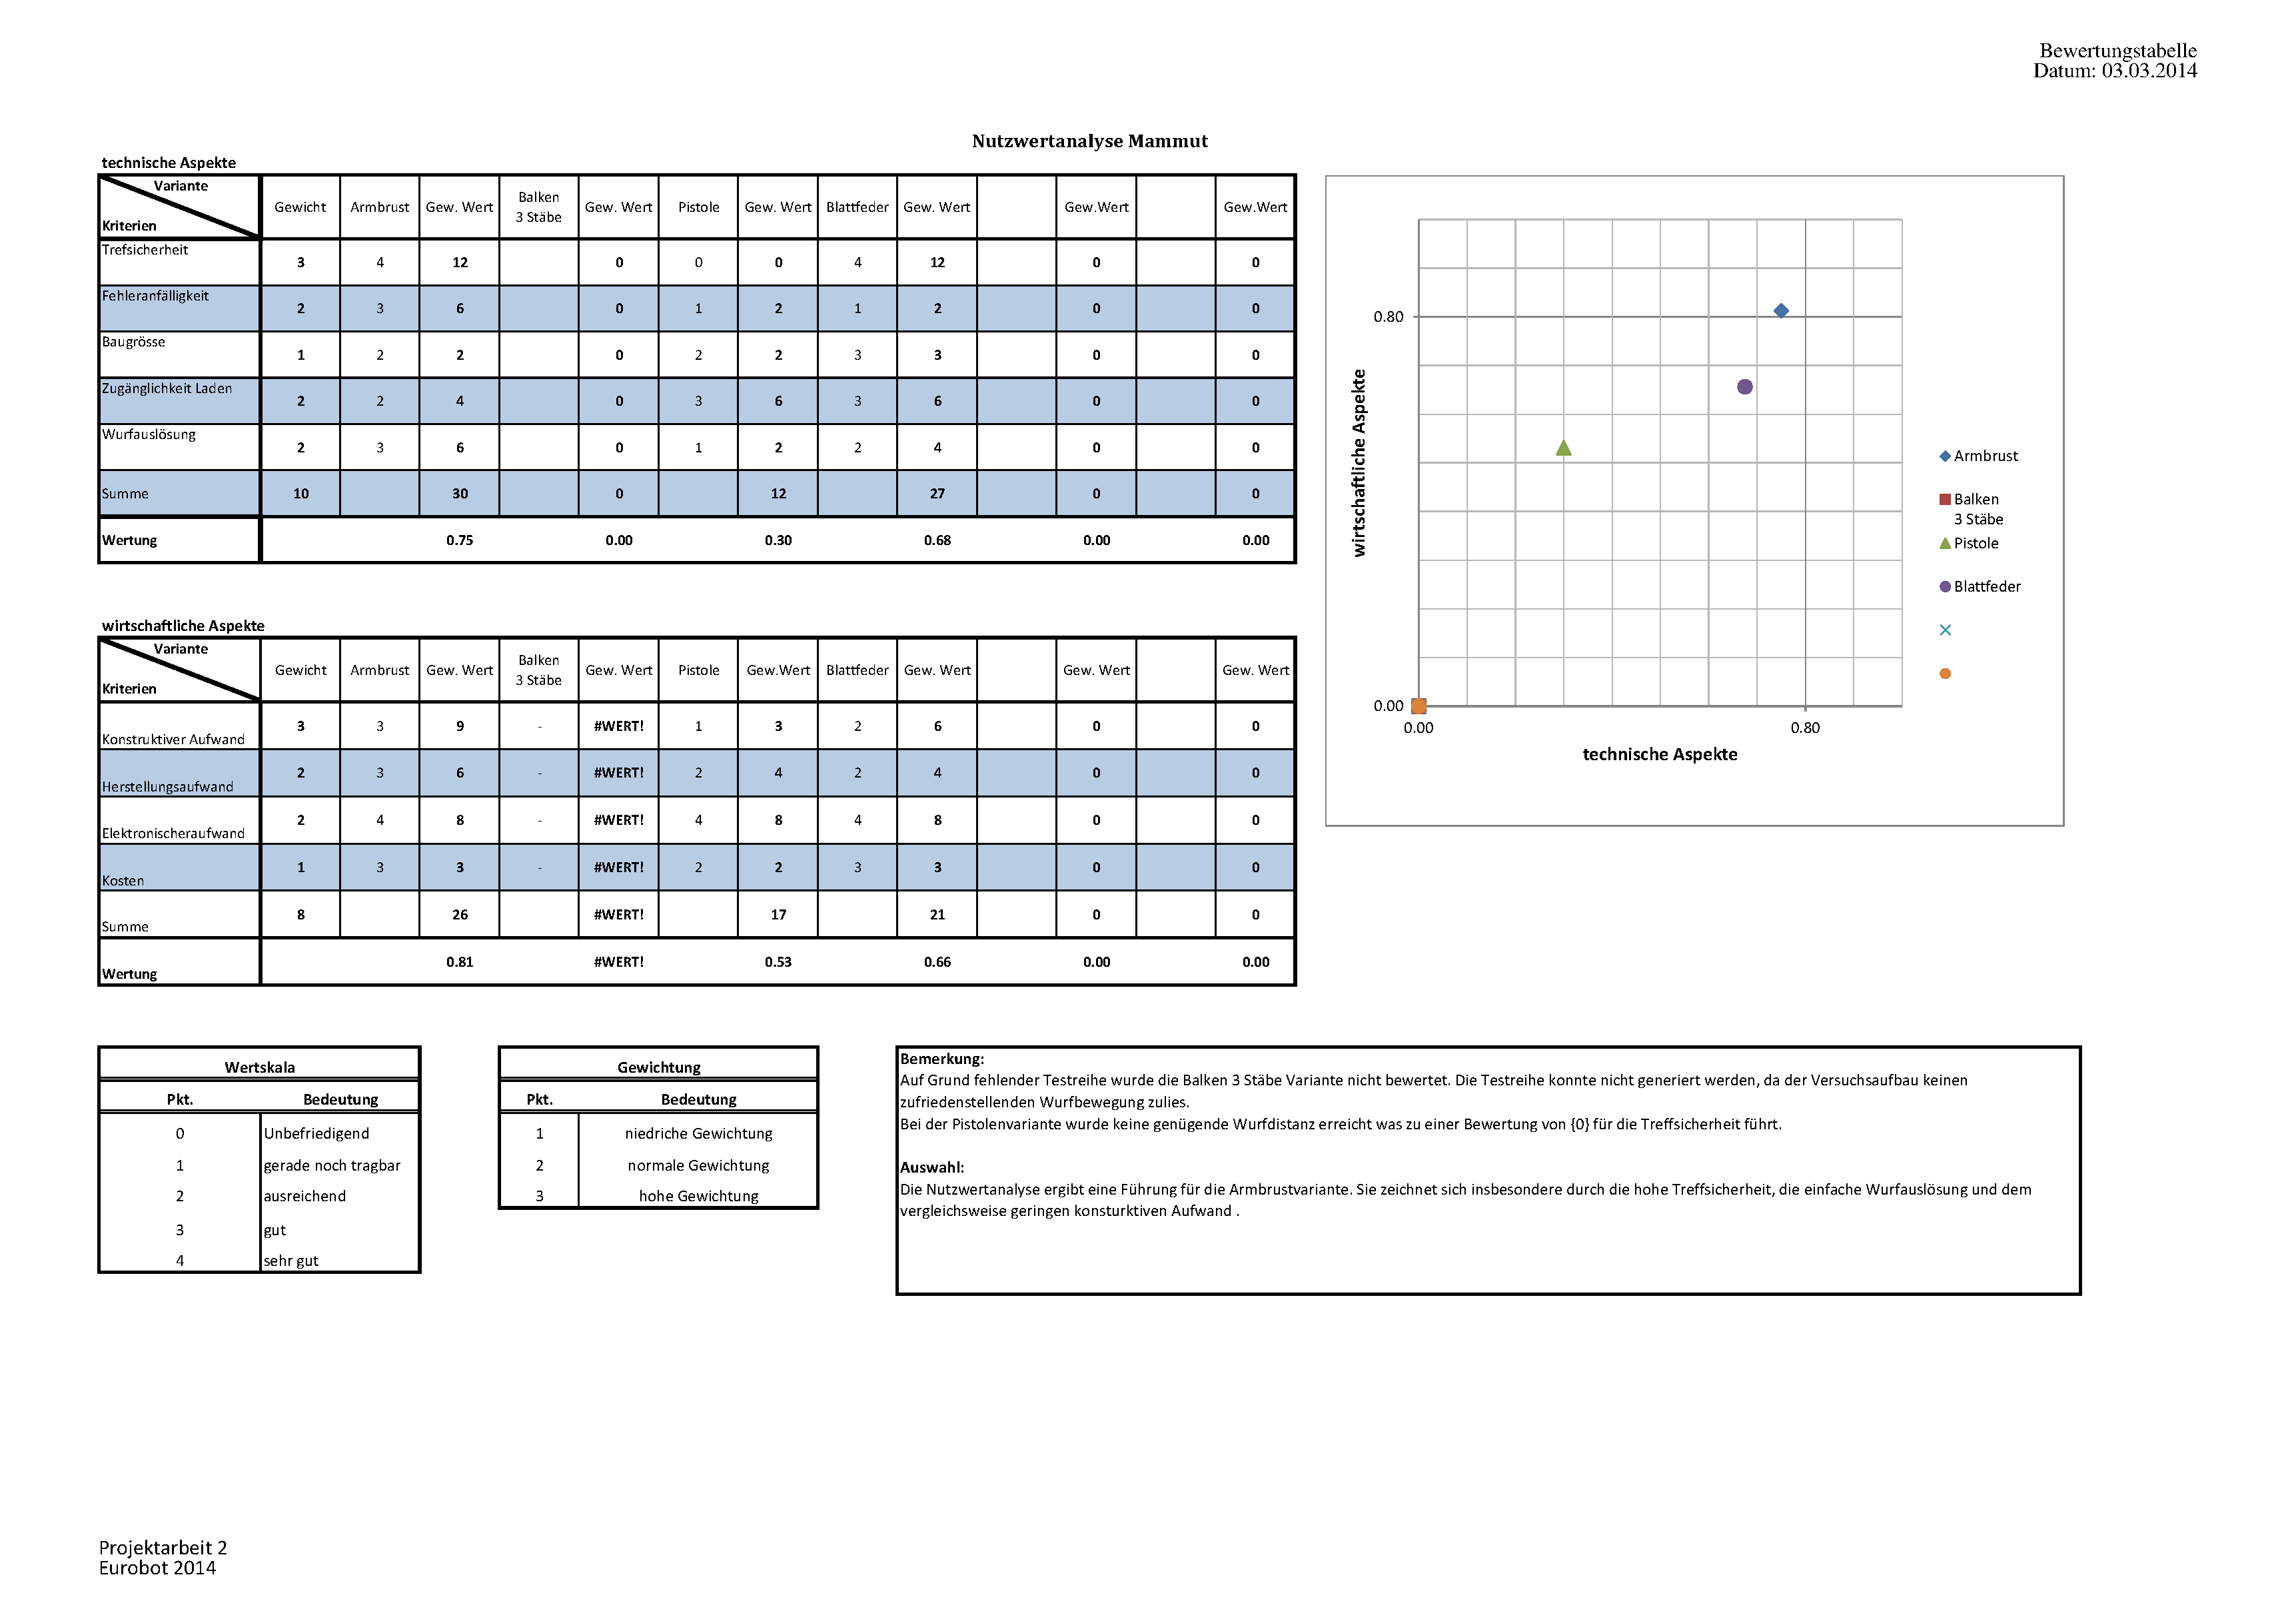
\includepdf[scale=0.80, pagecommand={}, pages=-, landscape=true]{appendix/Anhang_Mechanik_PA2/Konzept-_Ausarbeitungphase_mech/5S-Diagramm_Netz.pdf}
   	%
    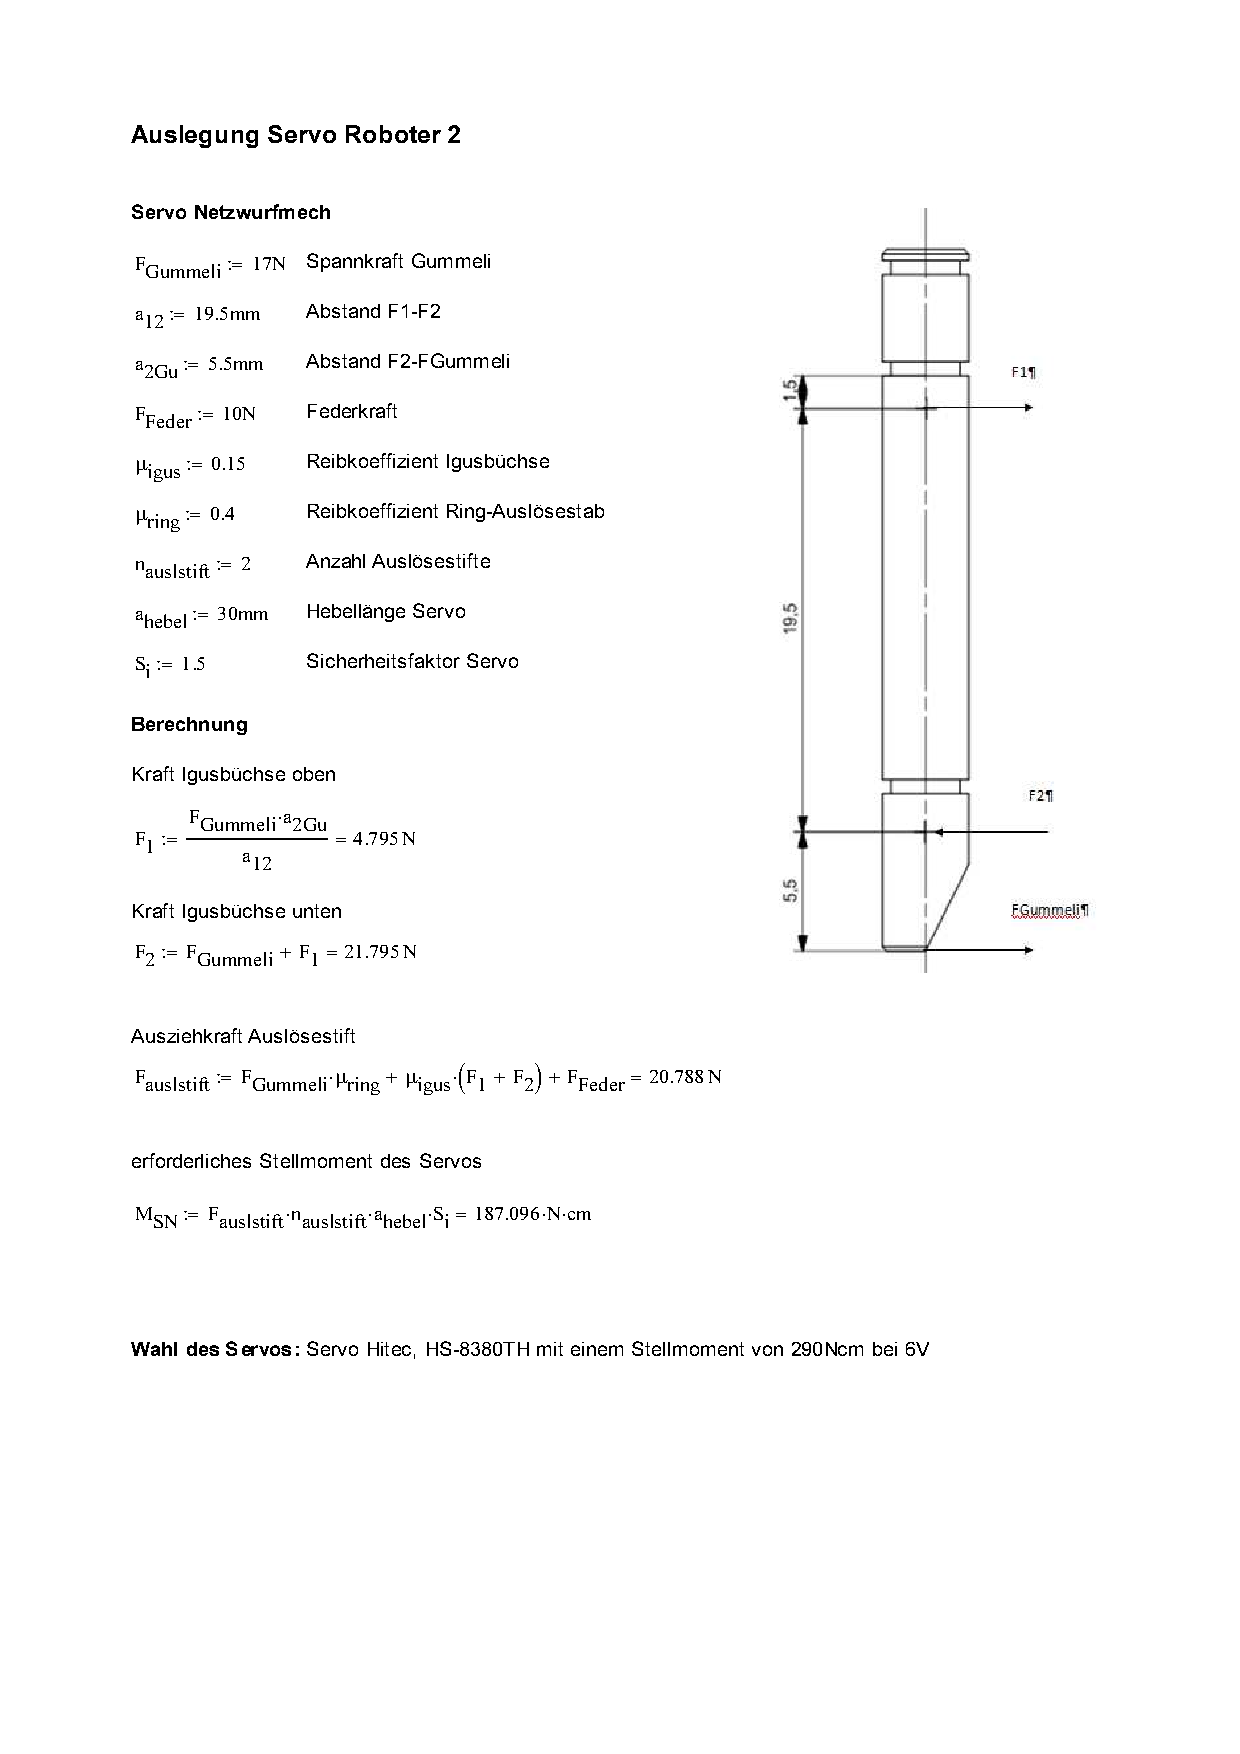
\includepdf[scale=0.80, pagecommand={}, pages=-, landscape=false]{appendix/Anhang_Mechanik_PA2/Konzept-_Ausarbeitungphase_mech/6Mathcad_Berechnung_Servos.pdf}
    %
%Anhang D
%%%%%%%%%%%%%%%%%%%%%%%%%%%%%%%%%%%%%%%%%%%%%%%%%%%%%%%%%%%%%%%%%%%%%%%%%%%%%%%
% Titel:   Bericht - Zeichnungen CAD
% Autor:   gross10
% Datum:   11.01.2014
% Version: 0.0.1
%%%%%%%%%%%%%%%%%%%%%%%%%%%%%%%%%%%%%%%%%%%%%%%%%%%%%%%%%%%%%%%%%%%%%%%%%%%%%%%
%
%:::Change-Log:::
% Versionierung erfolgt auf folgende Gegebenheiten: -1. Release Versionen
%                                                   -2. Neue Kapitel
%                                                   -3. Fehlerkorrekturen
%
% 0.0.01      Erstellung der Datei
%%%%%%%%%%%%%%%%%%%%%%%%%%%%%%%%%%%%%%%%%%%%%%%%%%%%%%%%%%%%%%%%%%%%%%%%%%%%%%% 
\chapter{Zeichnungen CAD}\label{ch:zeichnungen_cad}
	Alle konstruktiven Zeichnungen f�r die Aufgaben \gls{g:fresko}, \gls{g:mammut}, \gls{g:mammut_catch} und \gls{g:fire}.
	%
	\section{\gls{g:fresko}}
		Folgende Teile wurde f�r die Realisierung der \gls{g:fresko}-Aufgabe verwendetet.
		\begin{itemize}[parsep=1pt]
			\item Bild
			\item Linearmodul Grundplatte
			\item Winkelaufnehmer
			\item Bilderaufnahme
			\item Lagerung Winkelfehler
			\item Hebel Servo
			\item Achse Bilderaufnahme
			\item Winkelprofil 12x15x50
			\item Winkelprofil 12x15x80
			\item Igus Fuehrung
		\end{itemize} 
	%
	\section{\gls{g:mammut}}
		F�r die \gls{g:mammut}-Aufgabe wurden folgende Teile entworfen.
		\begin{itemize}[parsep=1pt]
			\item Speer
			\item Zufuerrohr
			\item Blattfeder
			\item Abschussblock
			\item Aufnahme Servo
			\item Abschussrampe
			\item Befestigungskurve links
			\item Befestigungskurve rechts
			\item Klemme Blattfeder
			\item Befestigungsplatte
			\item Hebel Servo
			\item Klinke
			\item Klinkenwelle
			\item Verbindungsblock
			\item Verbindungsachse
			\item Lagerung Klinkenwelle links
			\item Lagerung Klinkenwelle rechts
			\item Drehpunktachse
			\item Lagerbock Federspanner links
			\item Lagerbock Federspanner rechts
			\item Rippe
			\item Explosions Abwurfvorrichtung
			\item Abstuetzung links
			\item Abstuetzung rechts
			\item Rohrbefestigung
		\end{itemize} 
		%
		%
		\section{\gls{g:mammut_catch}}
			F�r die \gls{g:mammut_catch}-Aufgabe wurden folgende Teile entworfen.
			\begin{itemize}[parsep=1pt]
				\item TODO
	%			\item 
	%			\item 
	%			\item 
	%			\item 
	%			\item 
	%			\item 
	%			\item 
	%			\item 
	%			\item 
	%			\item 
	%			\item 
	%			\item 
	%			\item 
	%			\item 
	%			\item 
	%			\item 
	%			\item 
	%			\item 
	%			\item 
	%			\item 
			\end{itemize}
				%
			\section{\gls{g:fire}}
				F�r die \gls{g:fire}-Aufgabe wurden folgende Teile entworfen.
				\begin{itemize}[parsep=1pt]
					\item TODO
		%			\item 
		%			\item 
		%			\item 
		%			\item 
		%			\item 
		%			\item 
		%			\item 
		%			\item 
		%			\item 
		%			\item 
		%			\item 
				\end{itemize}
			\section{\"Anderungen}
				F�r die \"Anderungen wurden folgende Teile entworfen.
				\begin{itemize}[parsep=1pt]
					\item TODO
		%			\item 
		%			\item 
		%			\item 
		%			\item 
		%			\item 
		%			\item 
		%			\item 
		%			\item 
		%			\item 
		%			\item 
		%			\item 
		%			\item 
		%			\item 
		%			\item 
				\end{itemize}
		%
		%
		%Fresko
		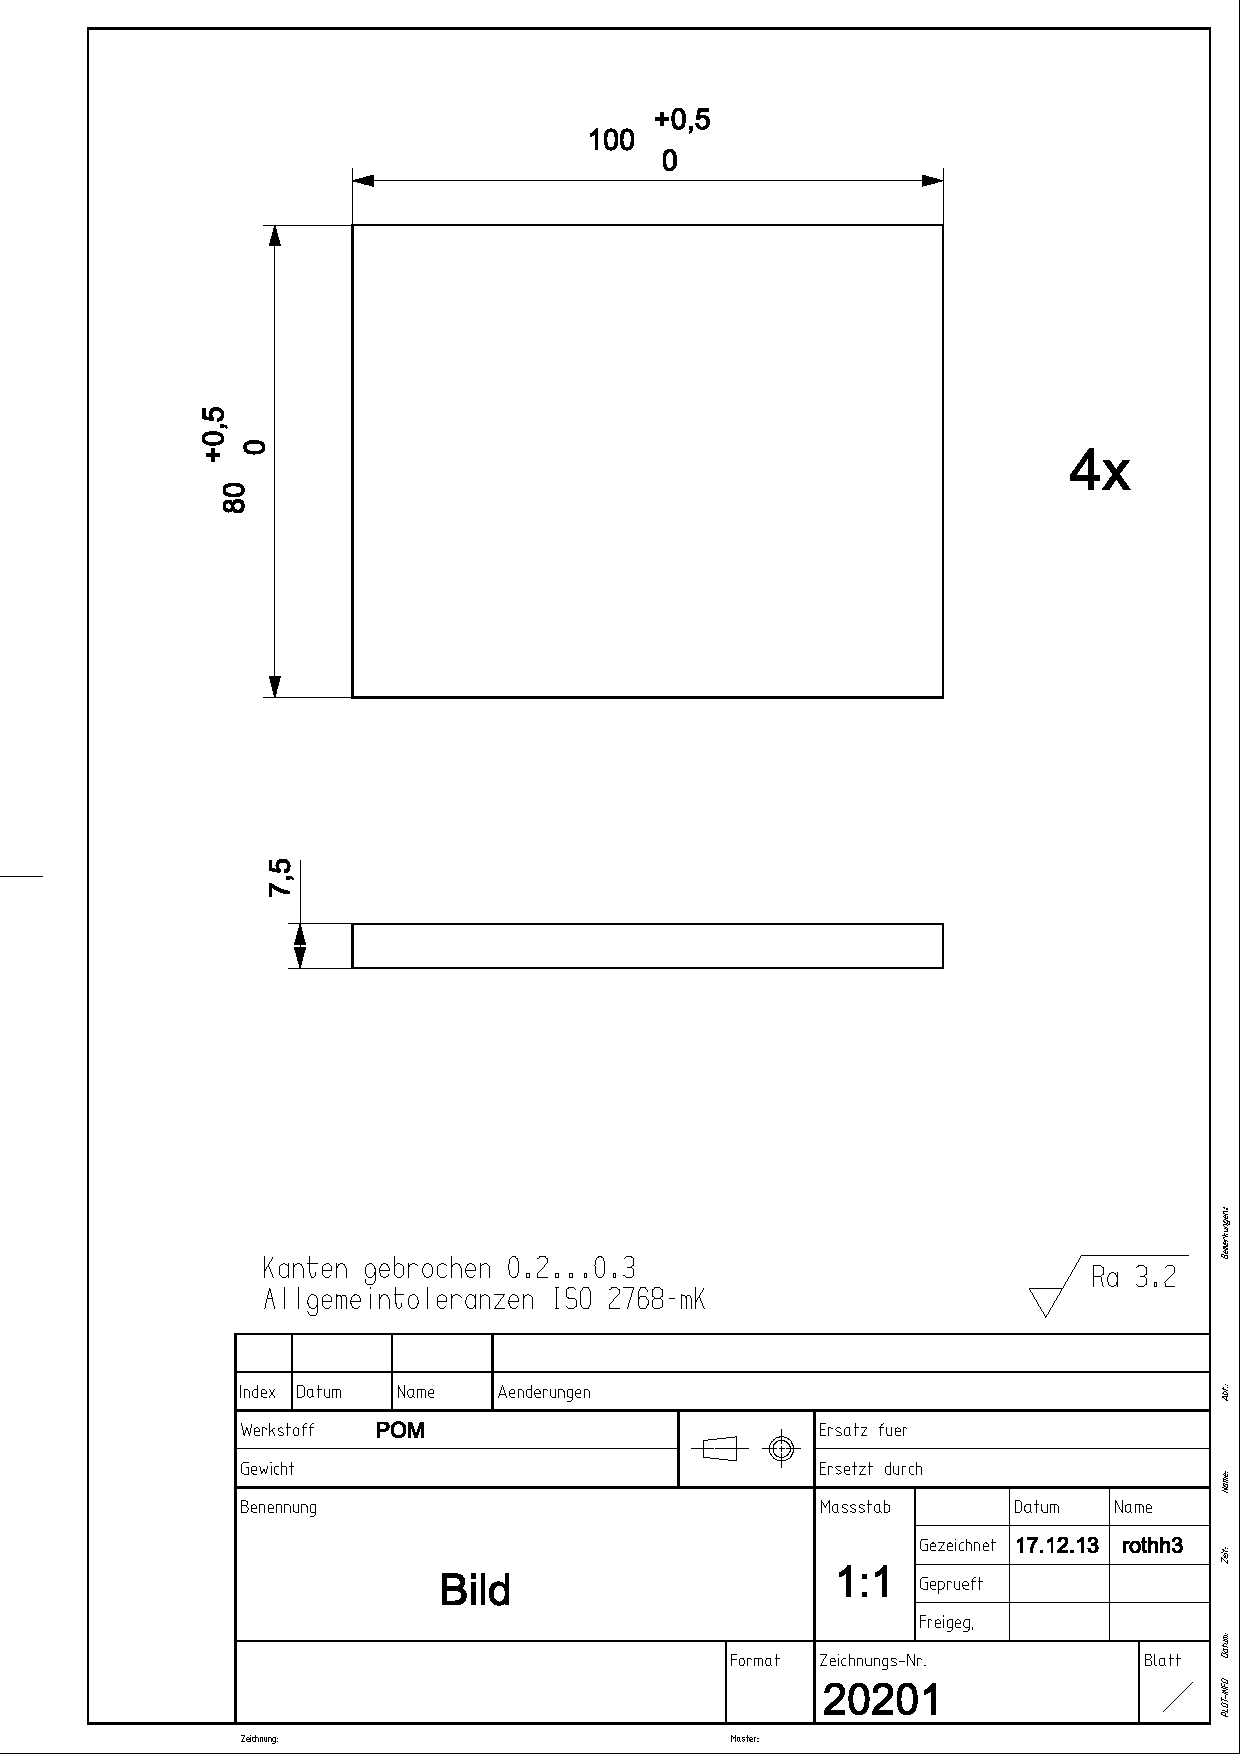
\includepdf[scale=0.7, pagecommand={}, pages=-]{appendix/image/Fresko/20201_Bild.pdf}
		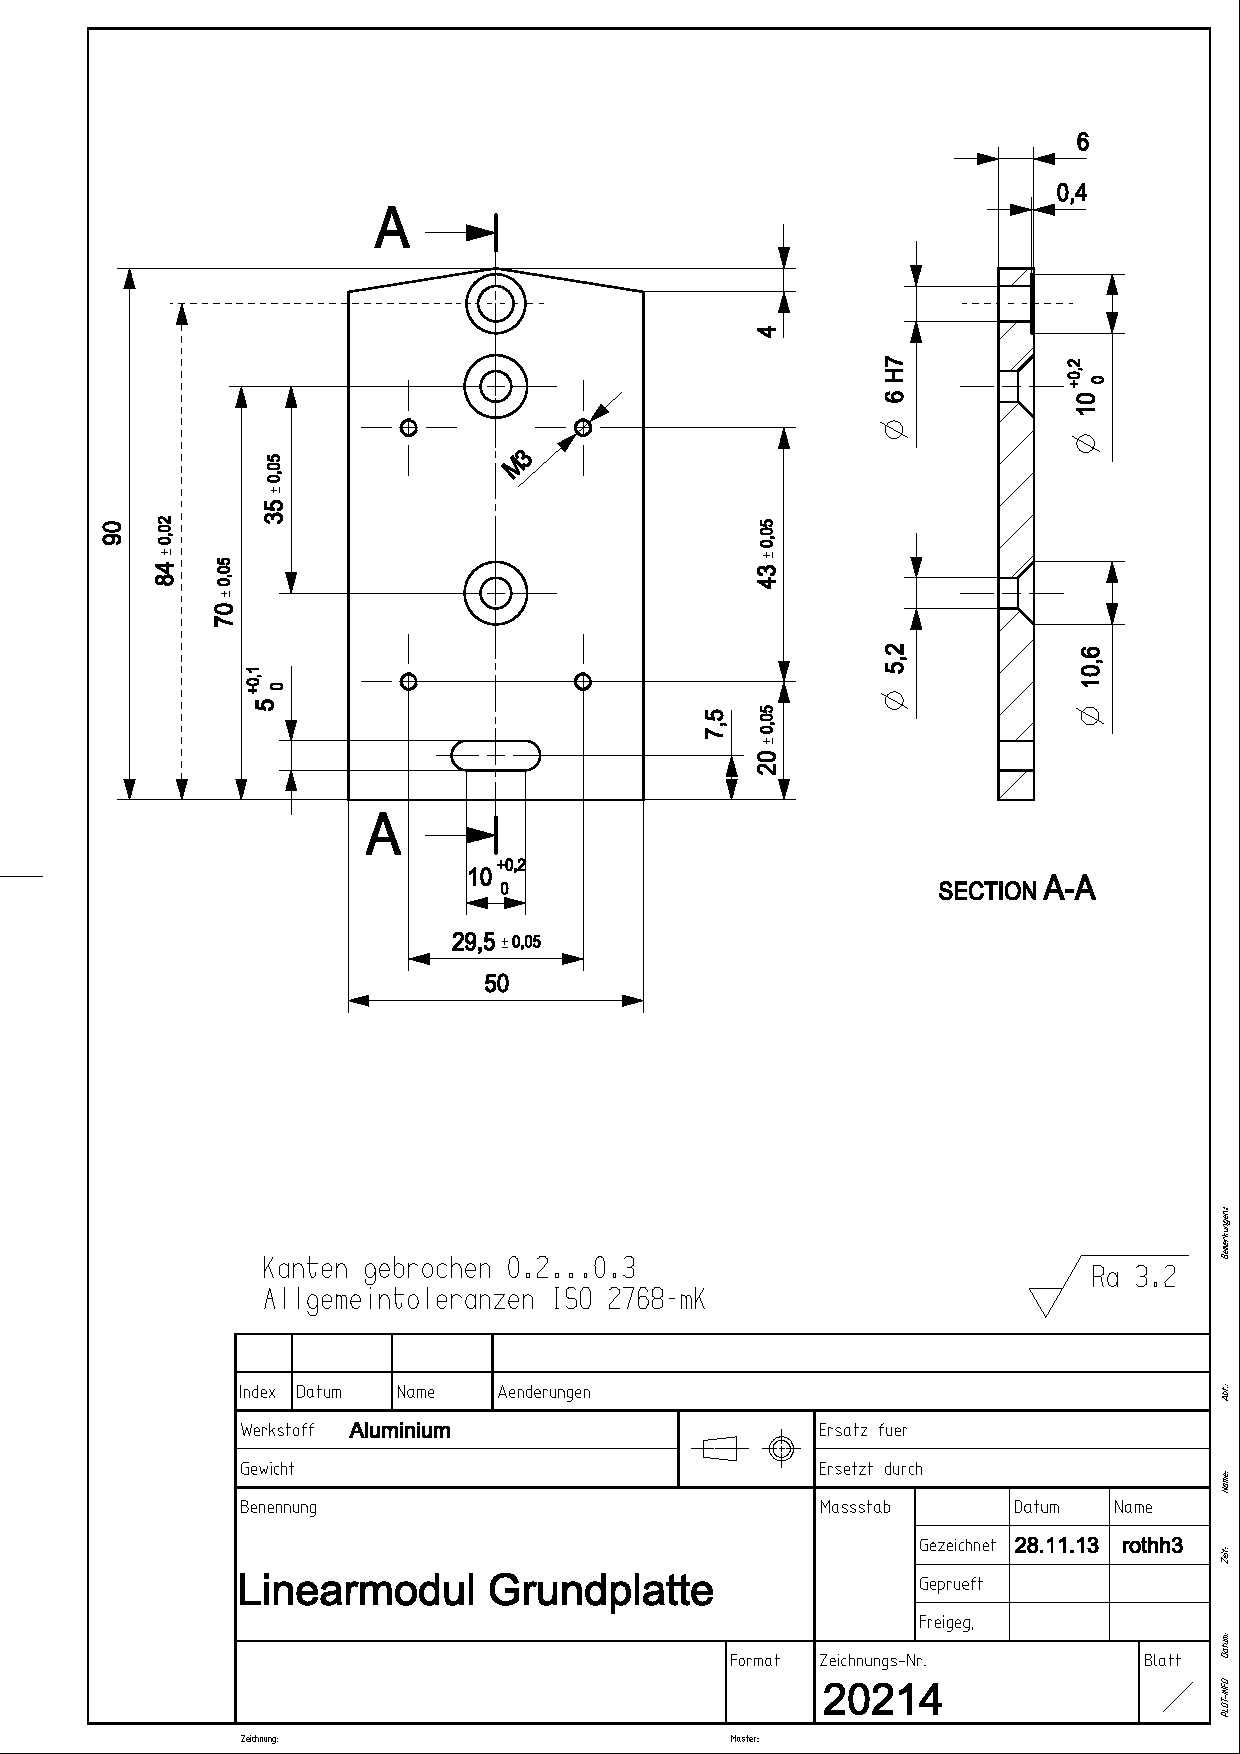
\includepdf[scale=0.7, pagecommand={}, pages=-]{appendix/image/Fresko/20214_Linearmodul_Grundplatte.pdf}
		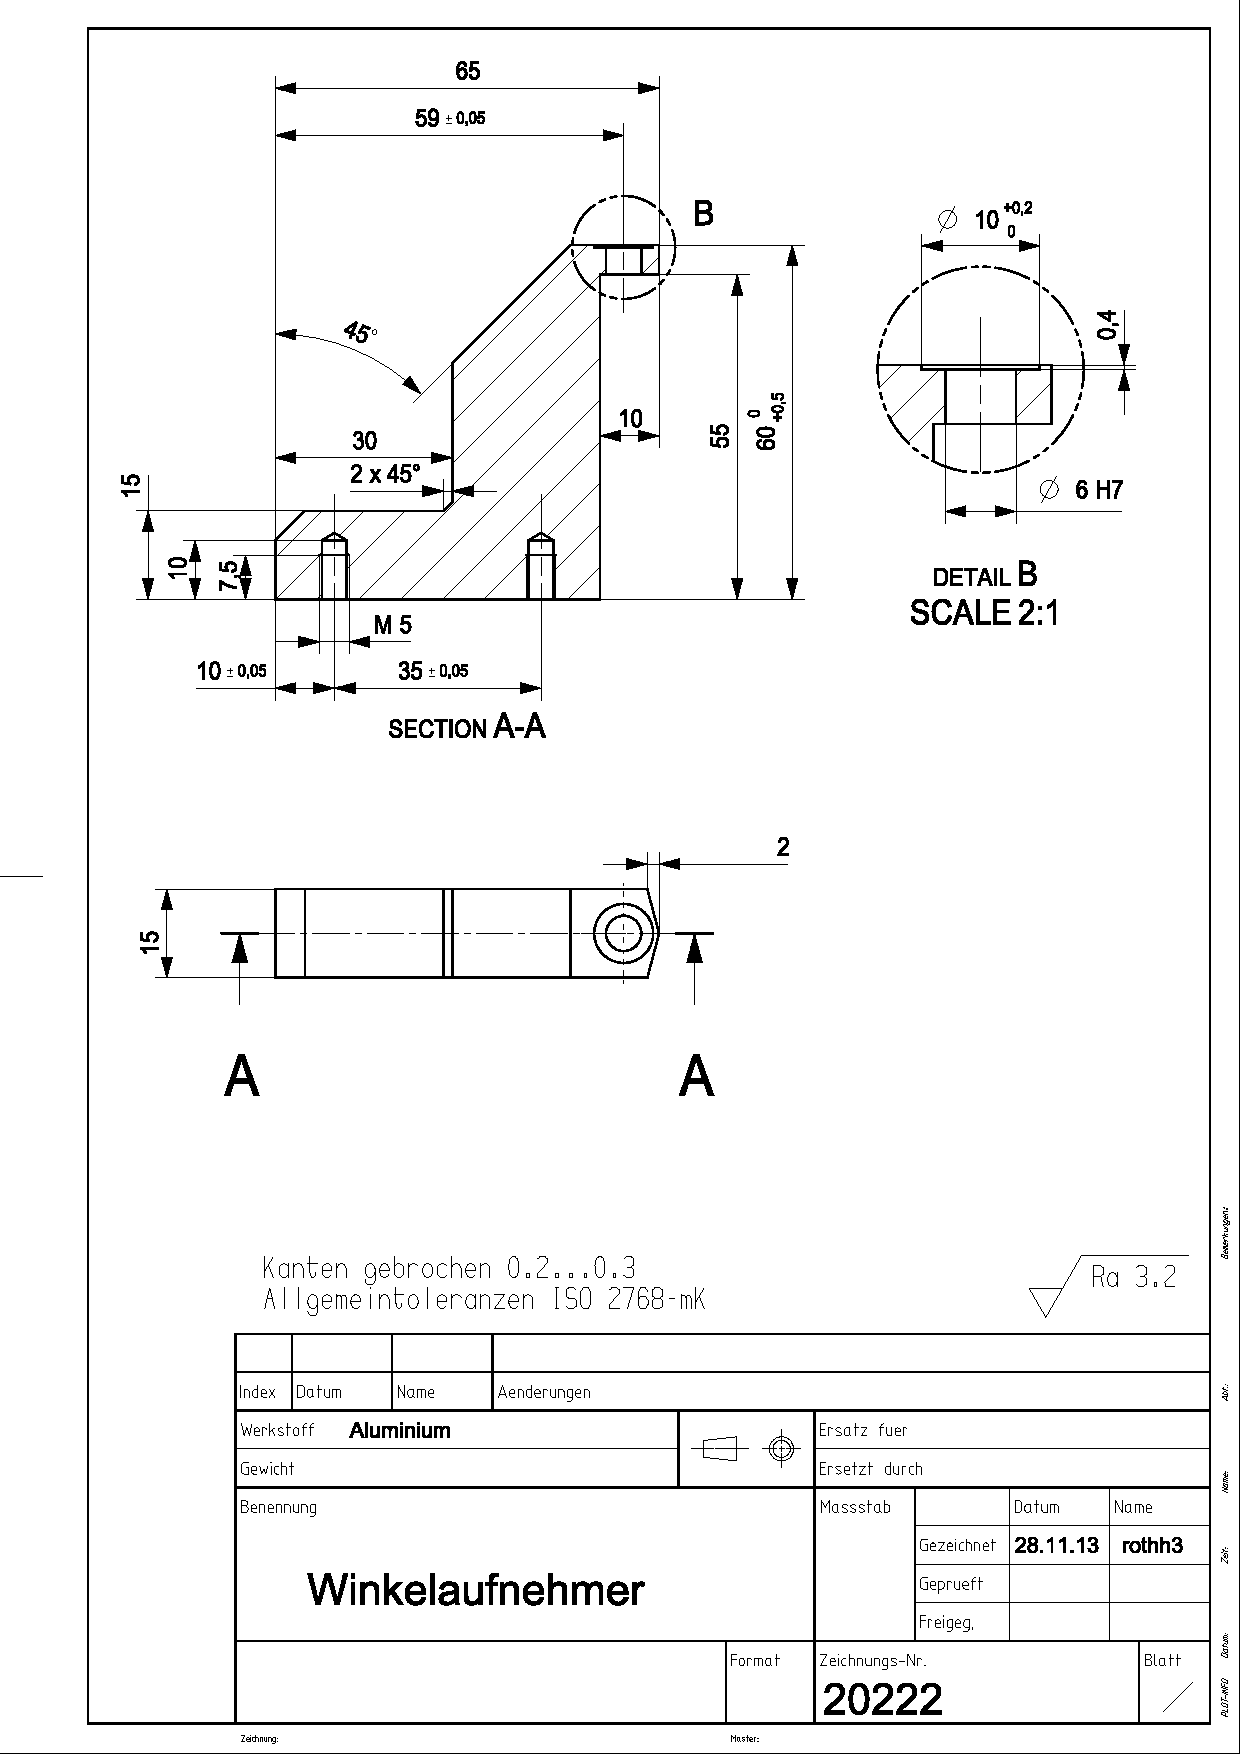
\includepdf[scale=0.7, pagecommand={}, pages=-]{appendix/image/Fresko/20222_Winkelaufneher.pdf}
		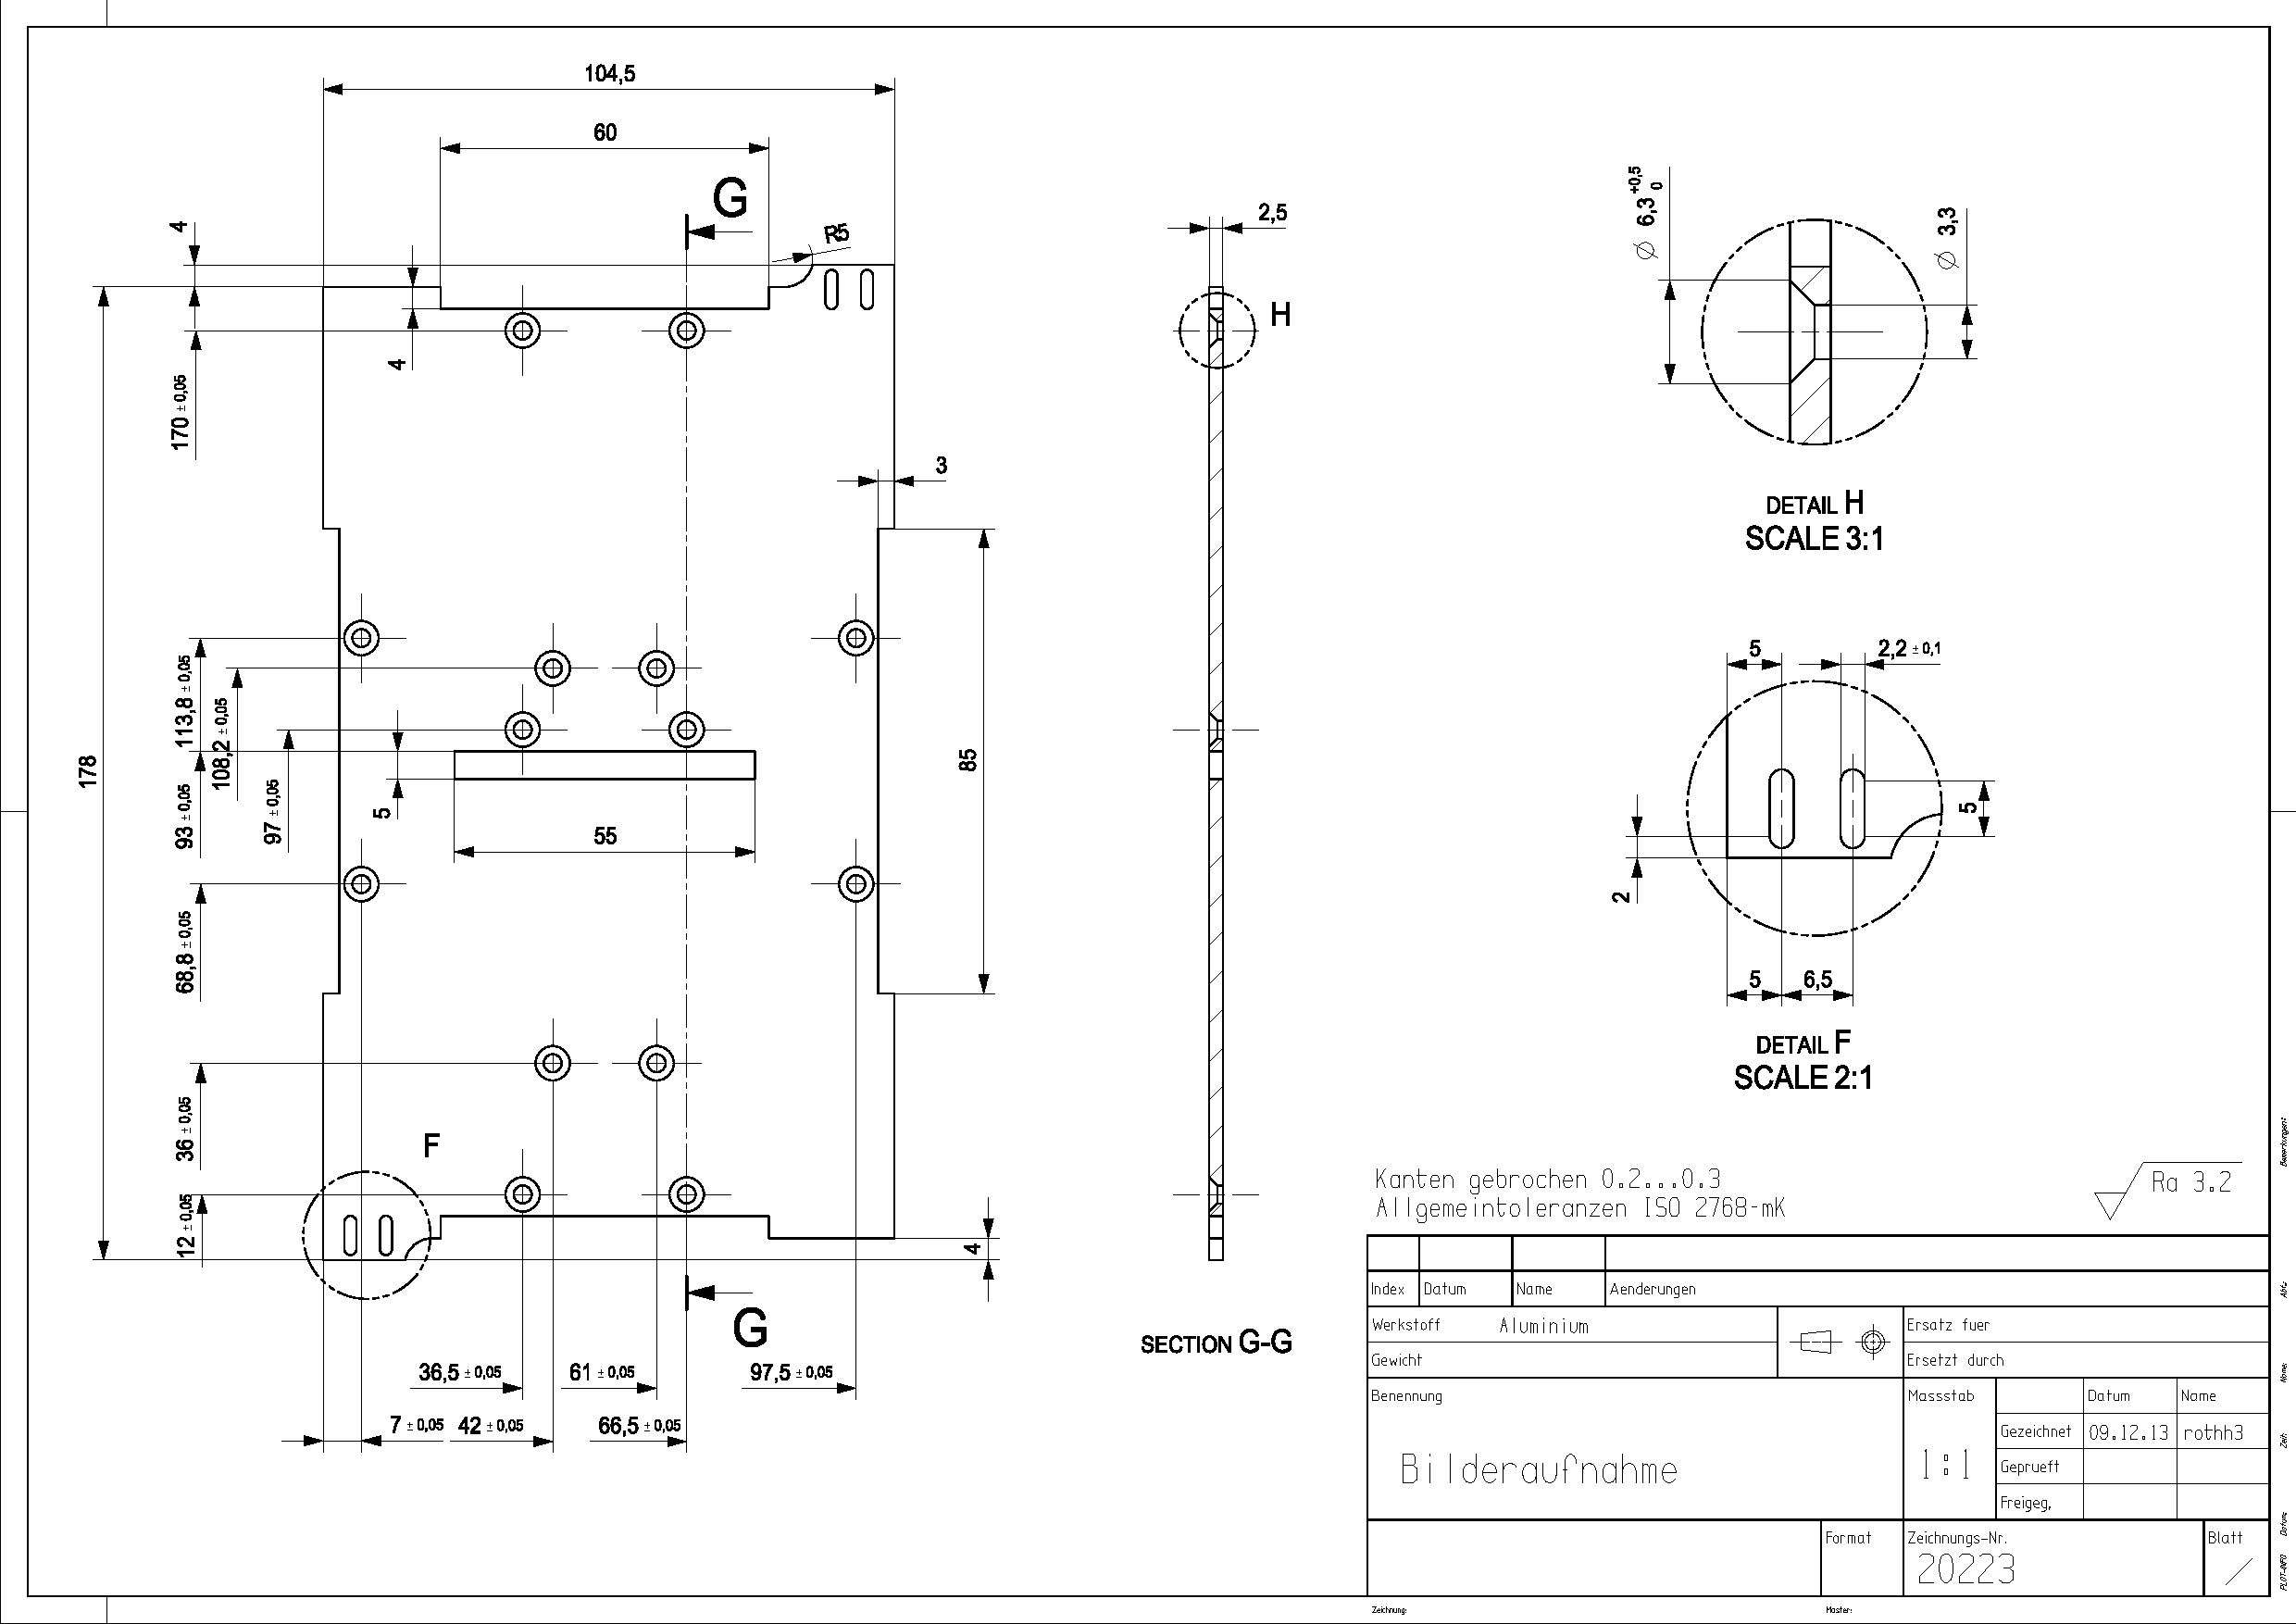
\includepdf[scale=0.7, pagecommand={}, pages=-, landscape=true]{appendix/image/Fresko/20223_Bilderaufnahme.pdf}
		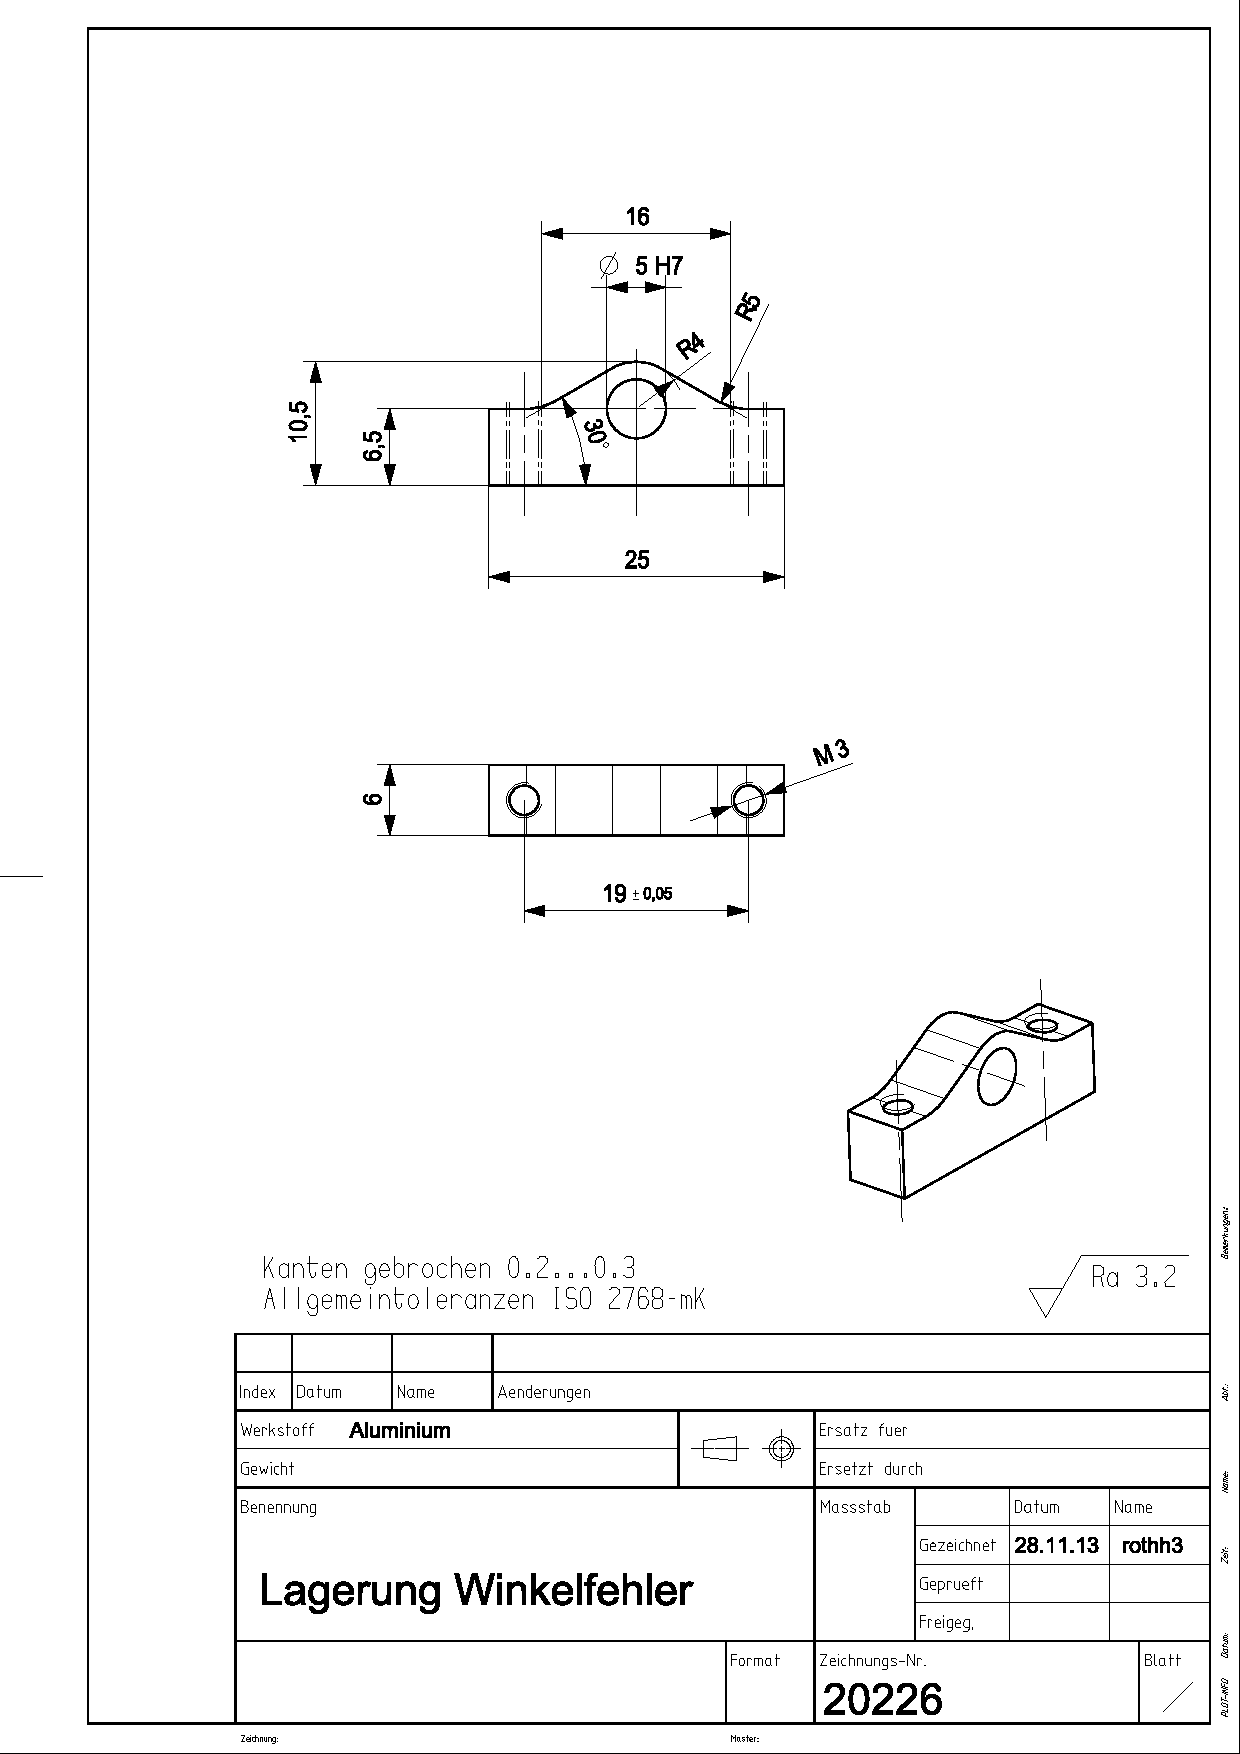
\includepdf[scale=0.7, pagecommand={}, pages=-]{appendix/image/Fresko/20226_Lagerung_Winkelfehler.pdf}
		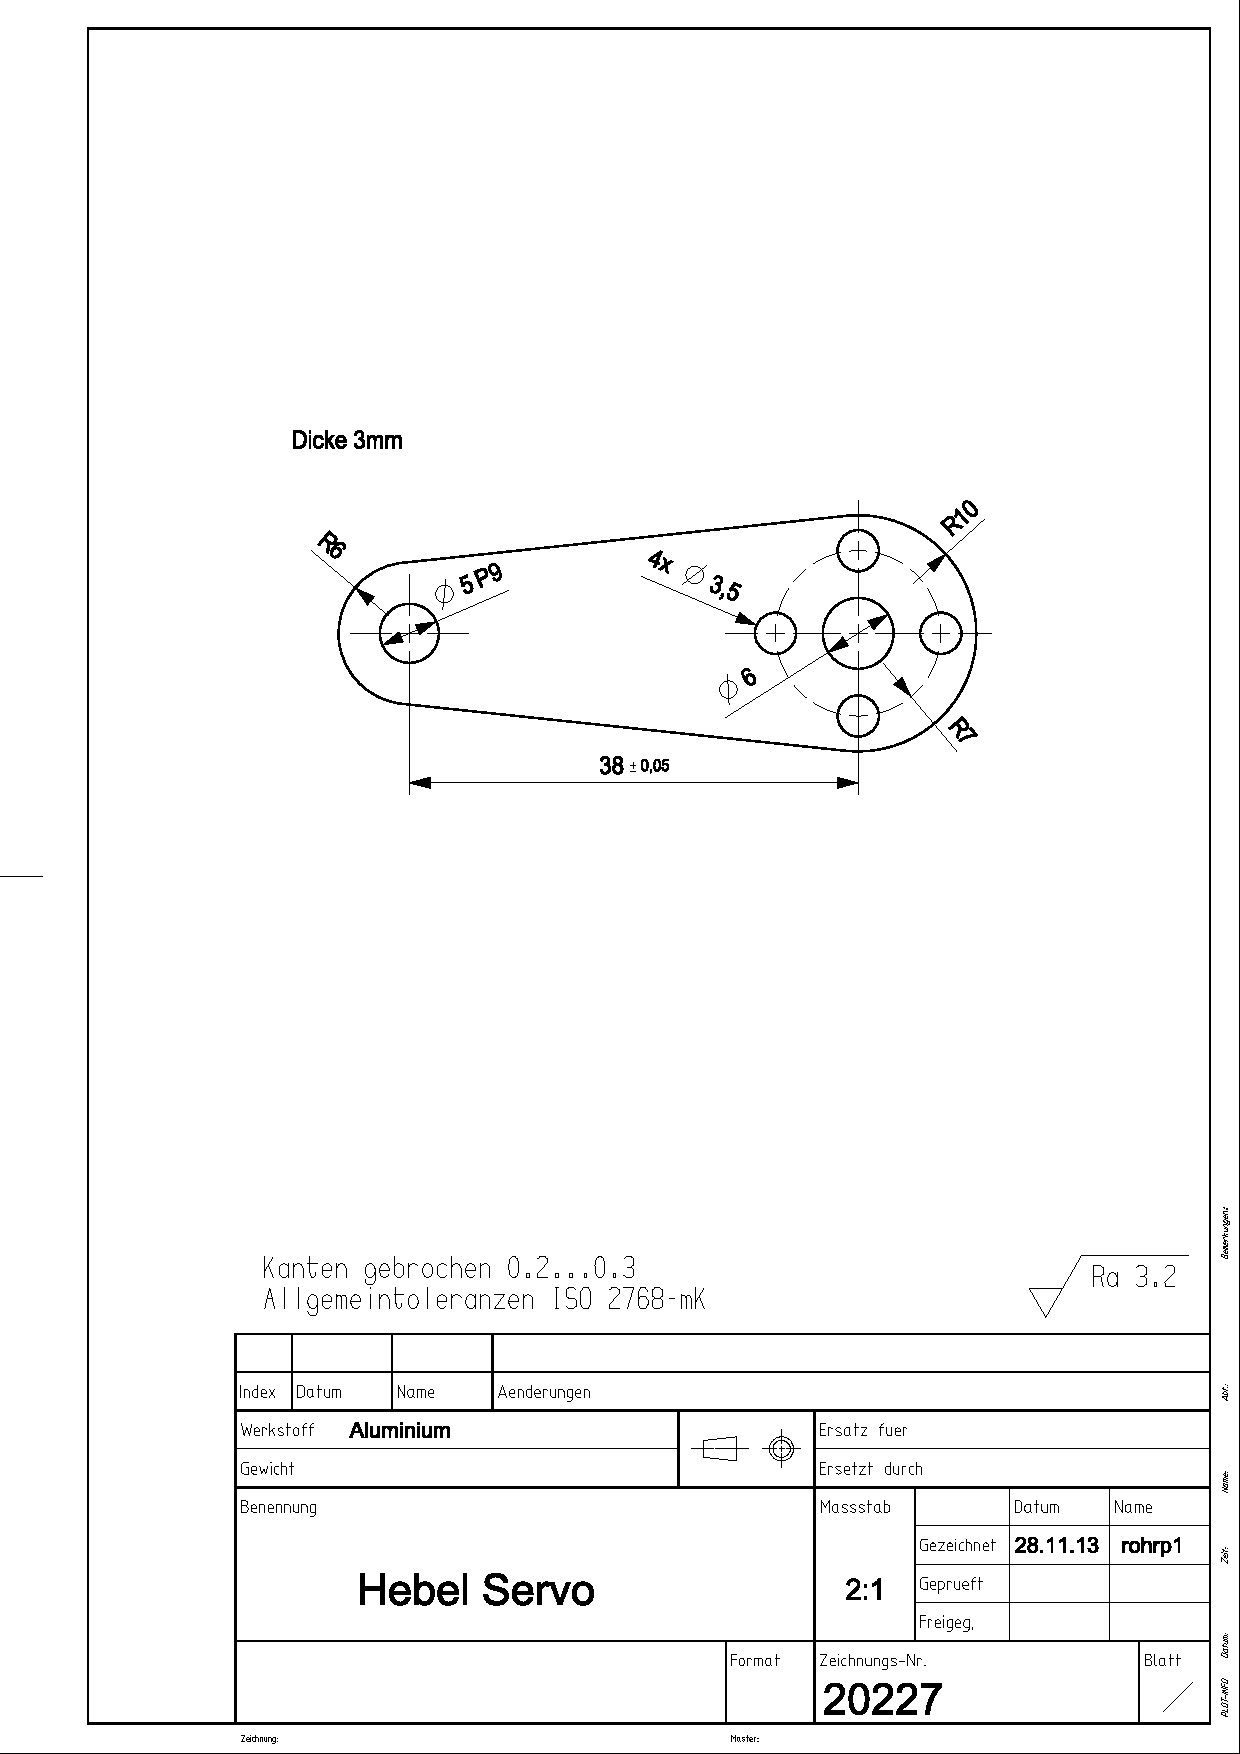
\includepdf[scale=0.7, pagecommand={}, pages=-]{appendix/image/Fresko/20227_Hebel_Servo.pdf}
		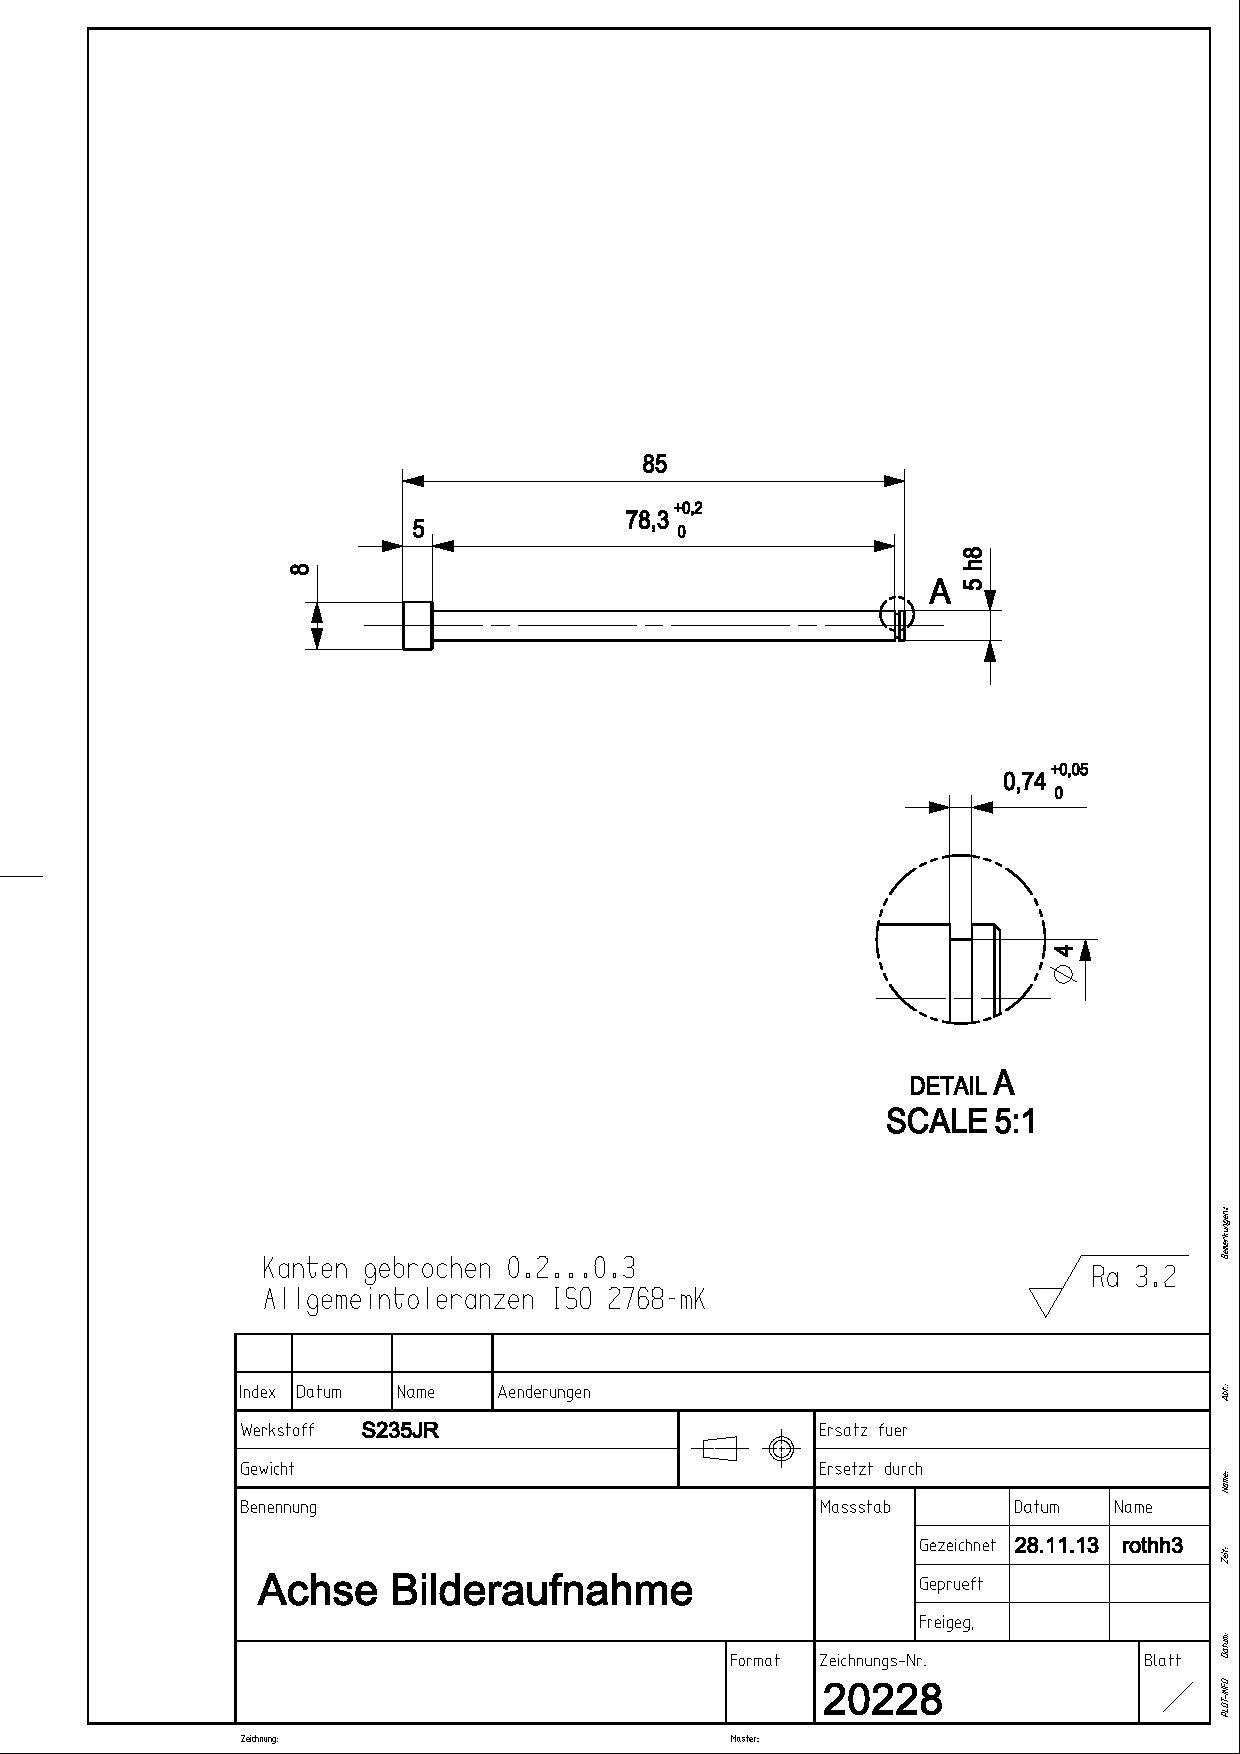
\includepdf[scale=0.7, pagecommand={}, pages=-]{appendix/image/Fresko/20228_Achse_Bilderaufnahme.pdf}
		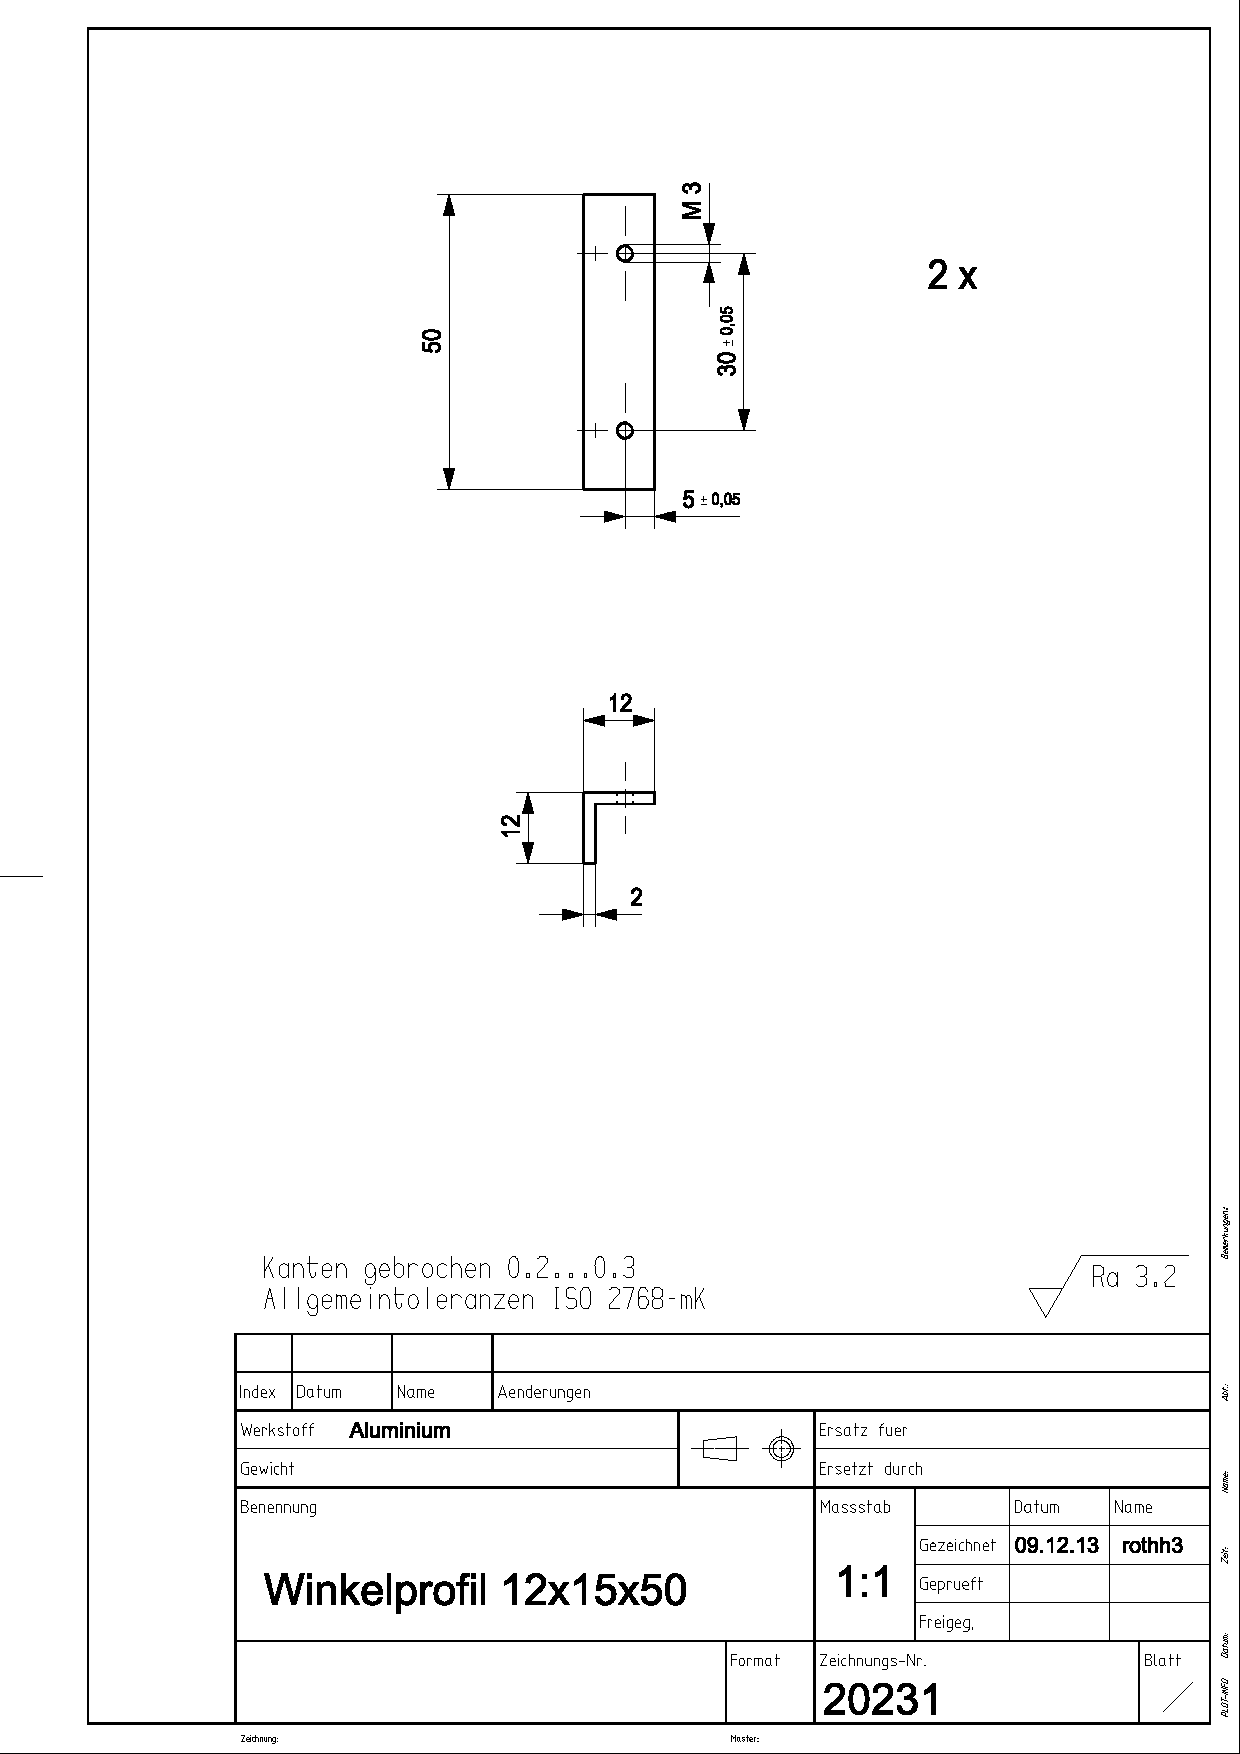
\includepdf[scale=0.7, pagecommand={}, pages=-]{appendix/image/Fresko/20231_Winkelprofil.pdf}
		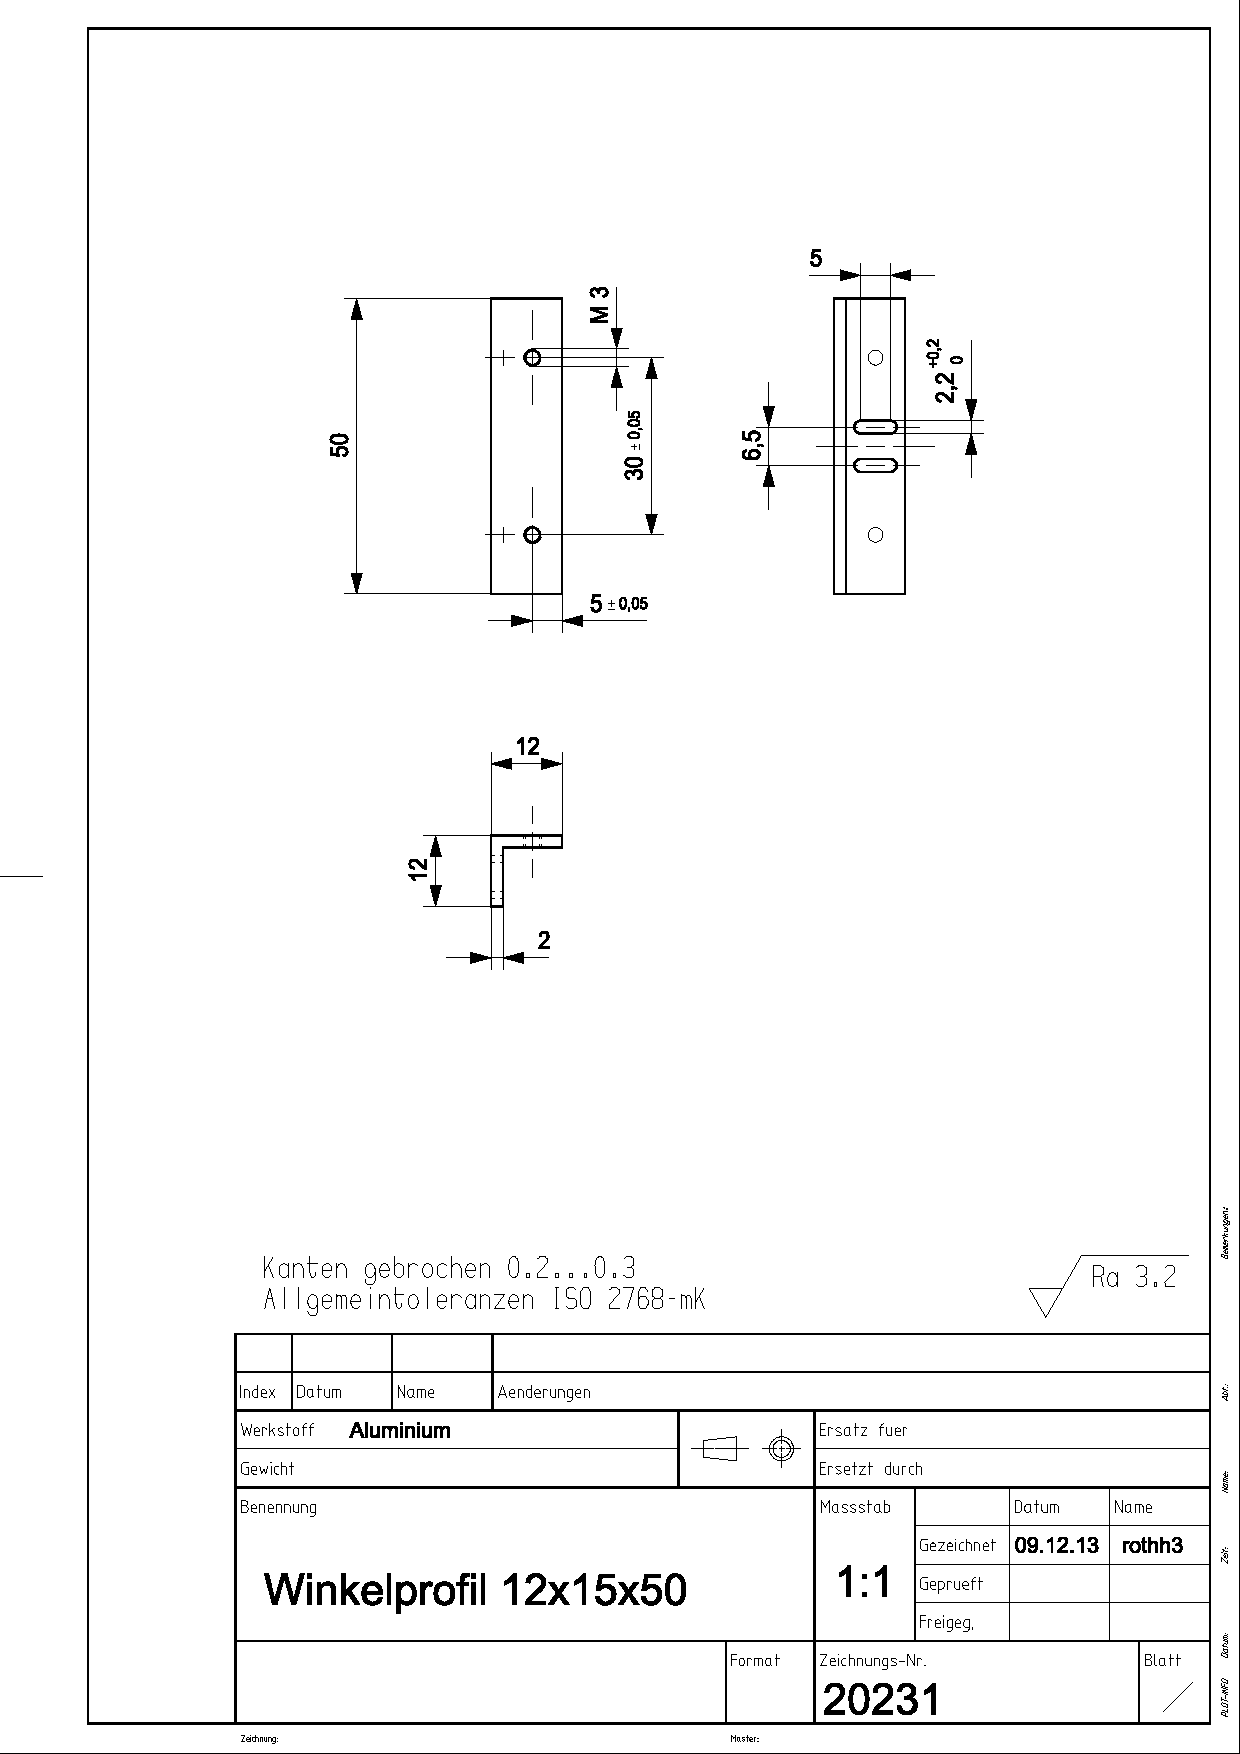
\includepdf[scale=0.7, pagecommand={}, pages=-]{appendix/image/Fresko/20231_Winkelprofil_mit_Nuten.pdf}
		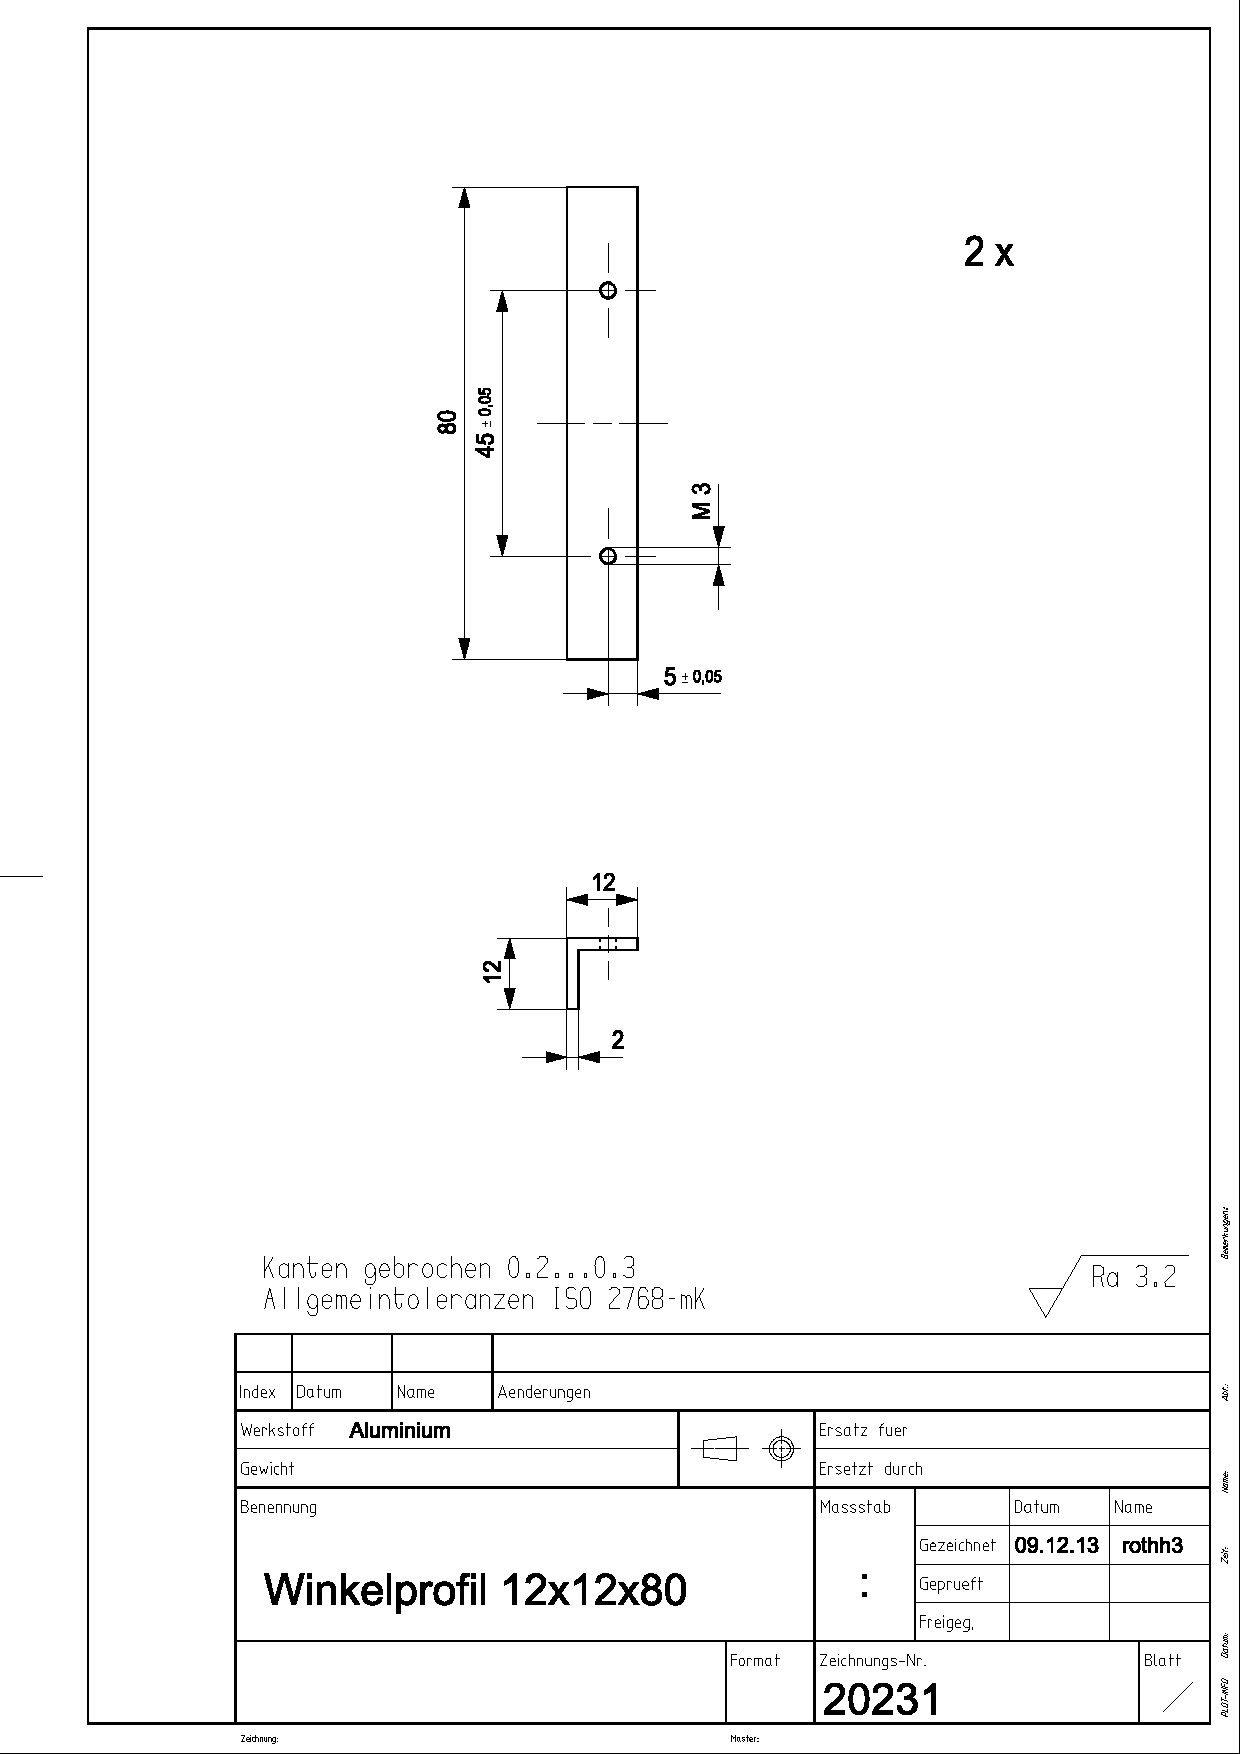
\includepdf[scale=0.7, pagecommand={}, pages=-]{appendix/image/Fresko/20231_WinkelprofilB.pdf}
		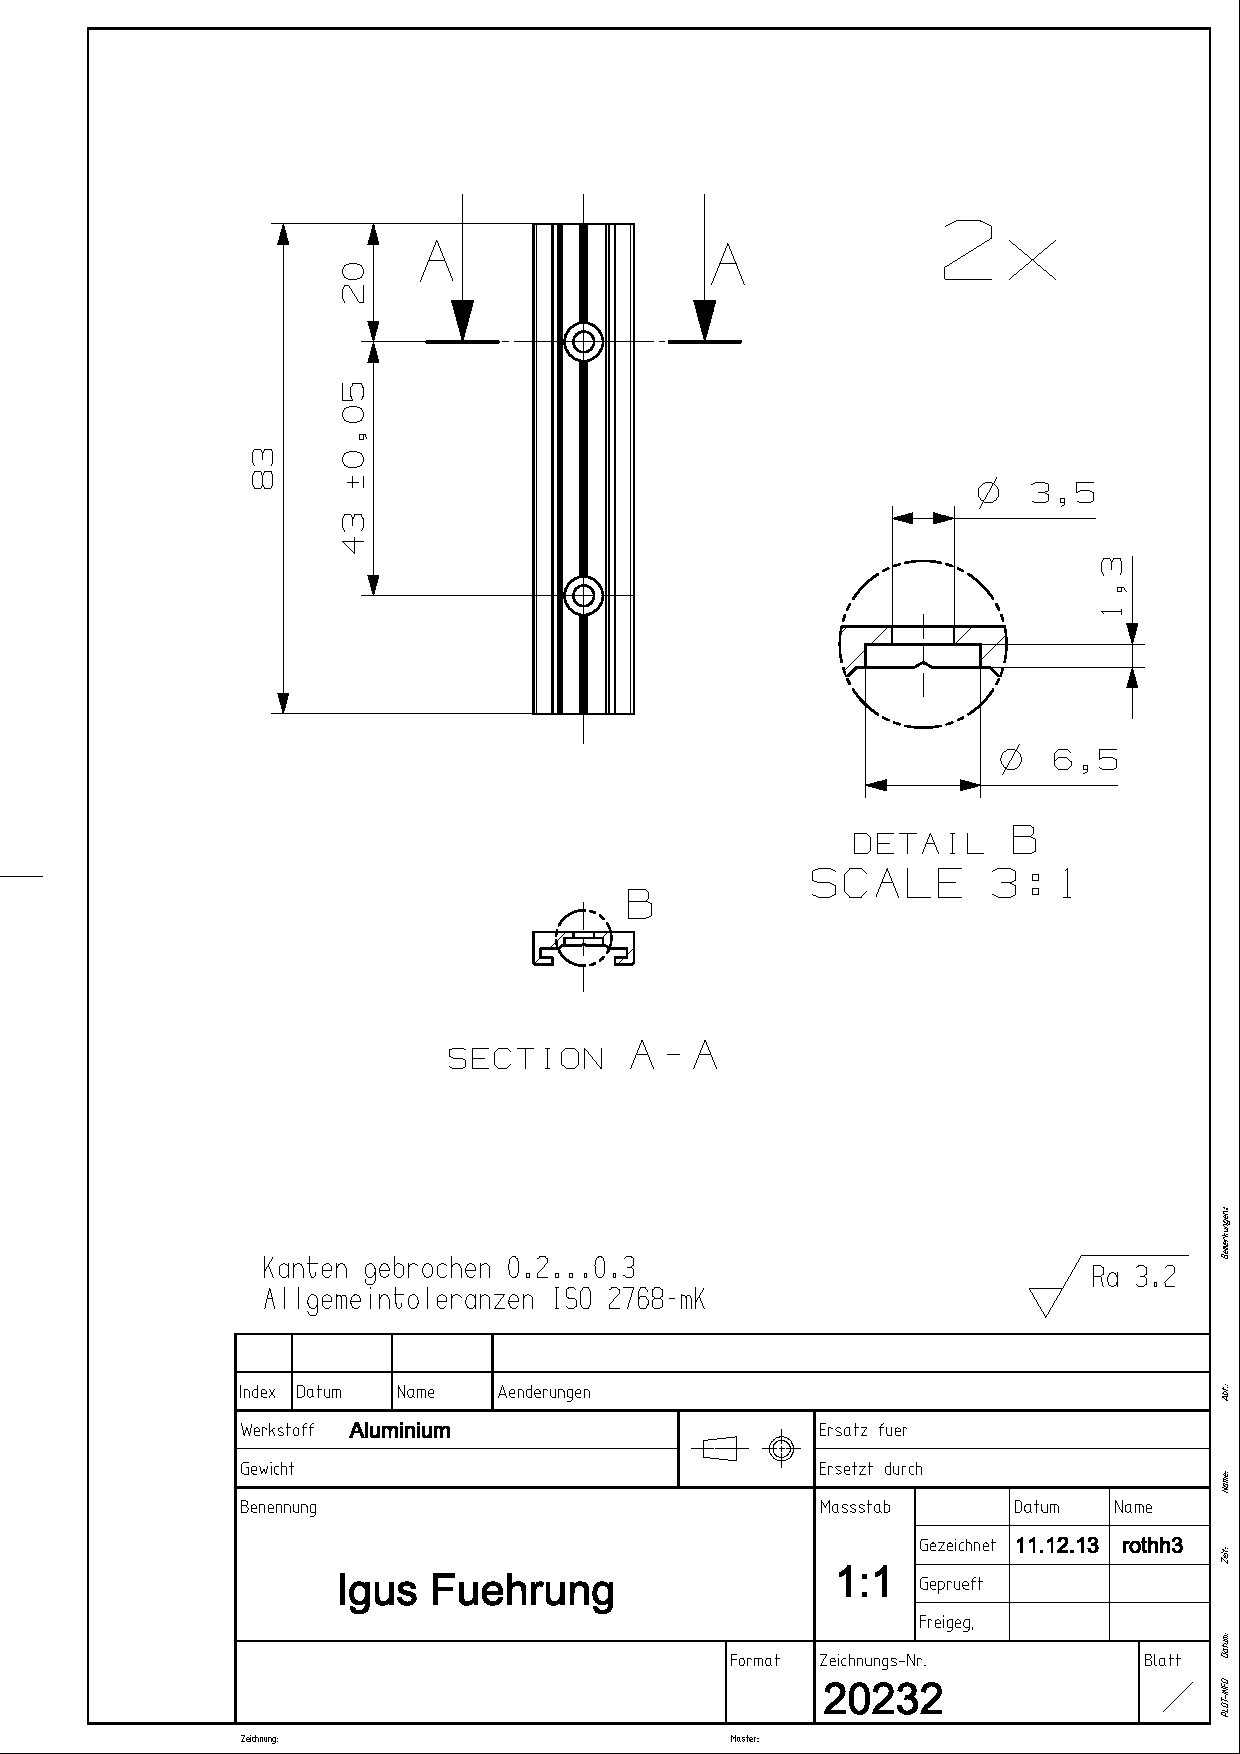
\includepdf[scale=0.7, pagecommand={}, pages=-]{appendix/image/Fresko/20232_Igus_Fuehrung.pdf}
		%
		%
		%Mammut
		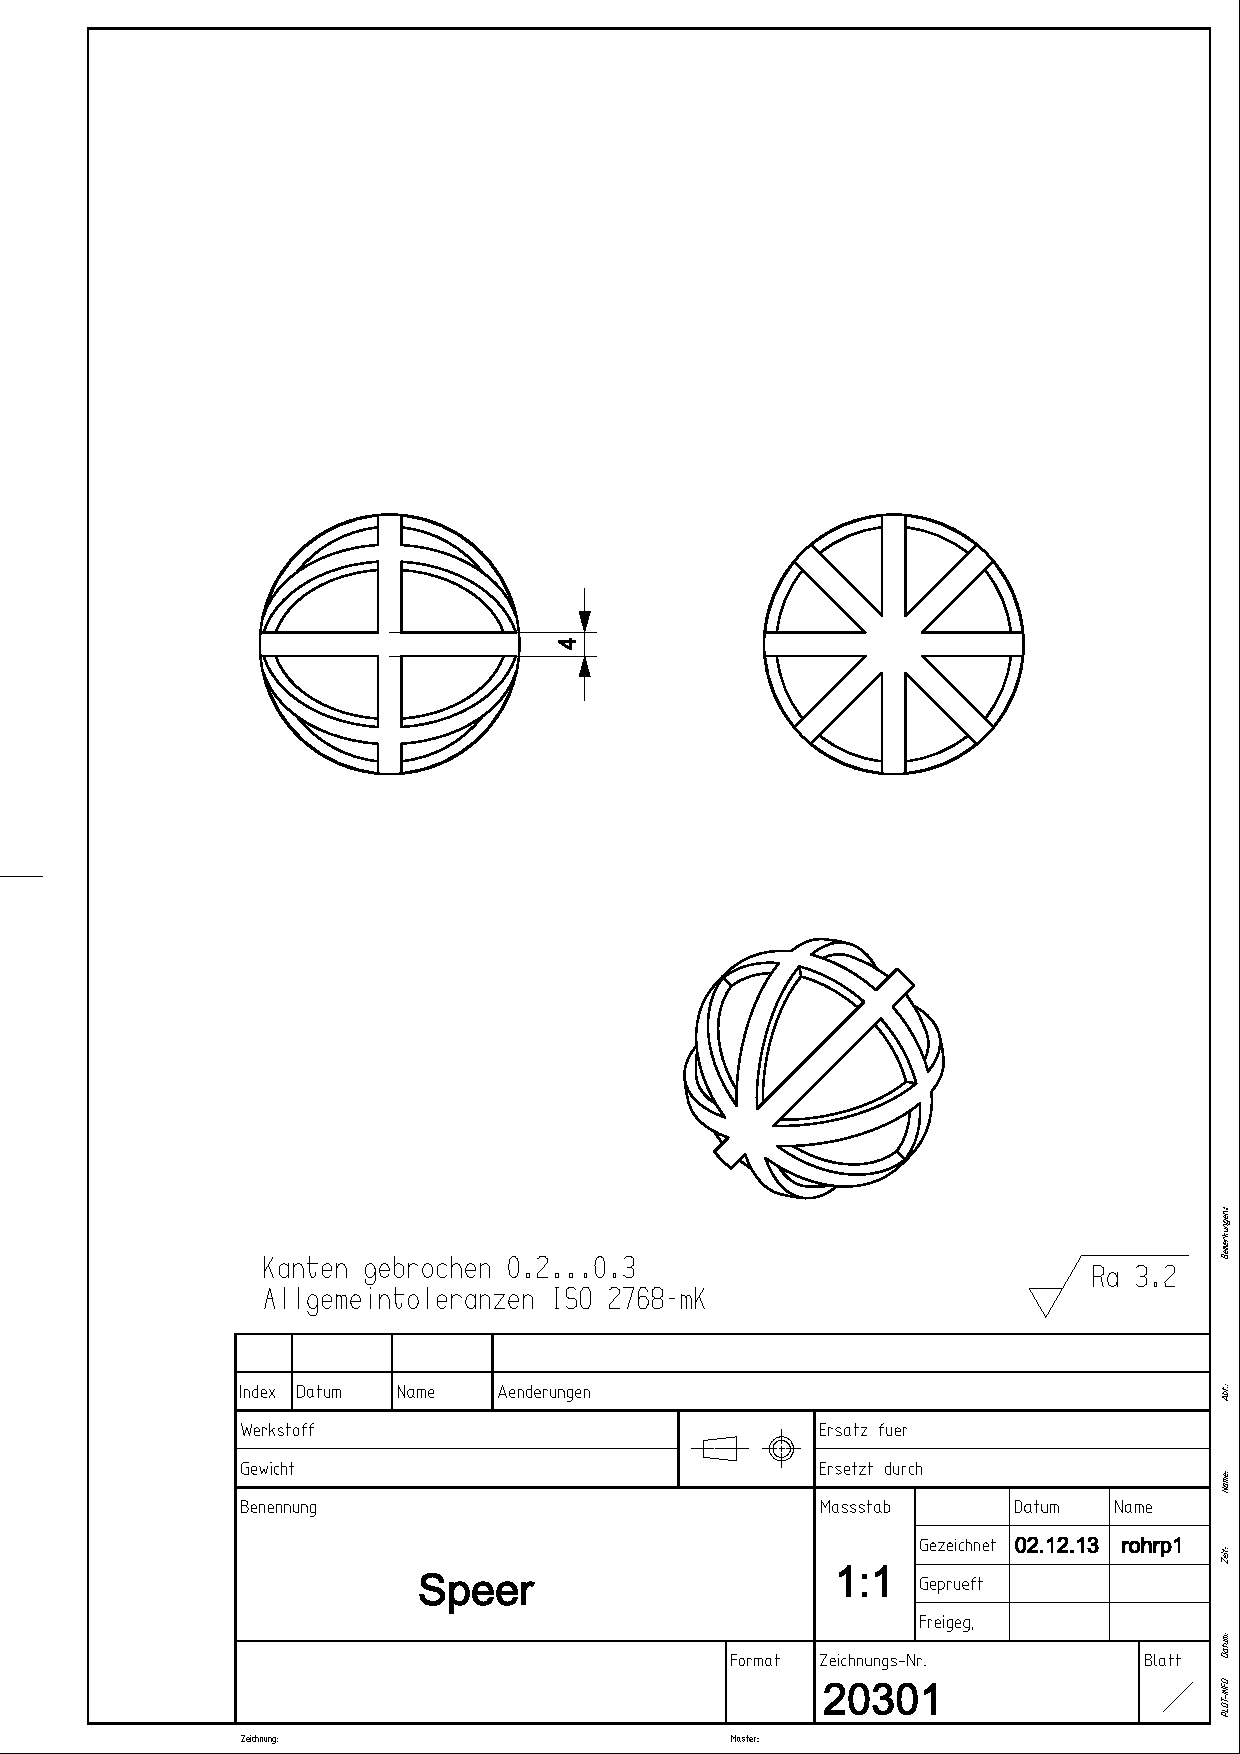
\includepdf[scale=0.7, pagecommand={}, pages=-]{appendix/image/Mammut/20301_Speer.pdf}
		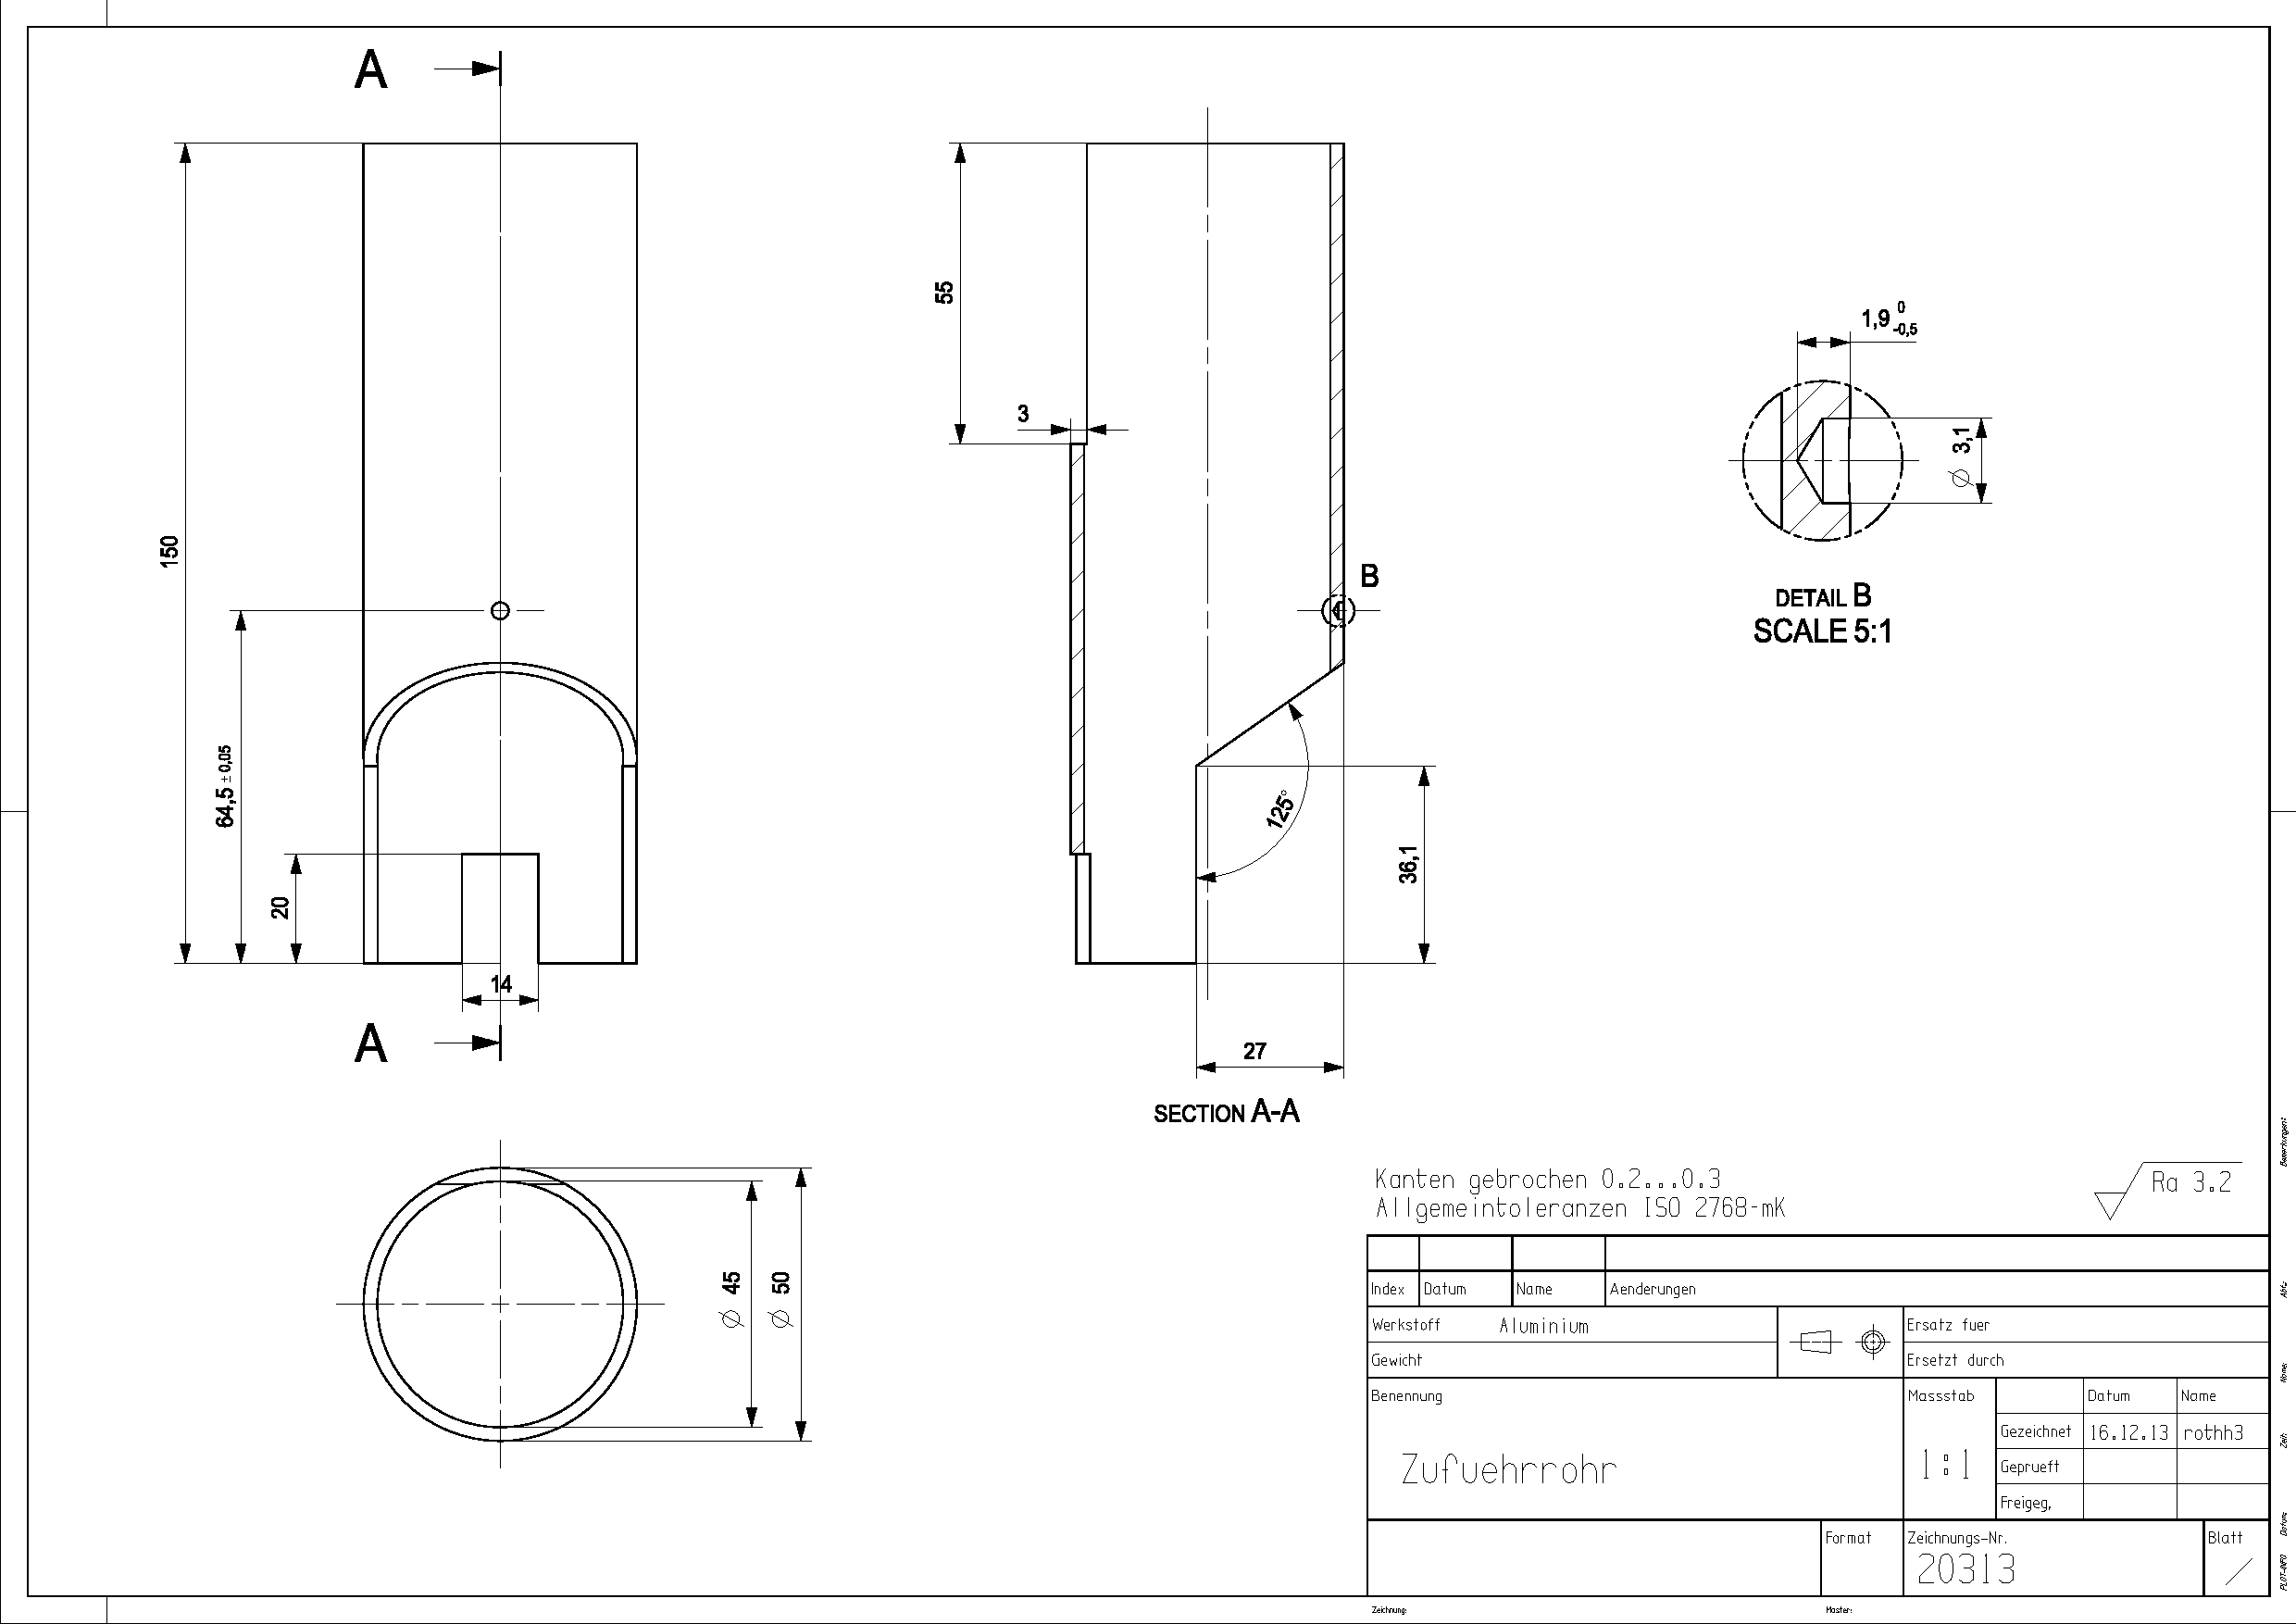
\includepdf[scale=0.7, pagecommand={}, pages=-, landscape=true]{appendix/image/Mammut/20313_Zufuehrrohr.pdf}
		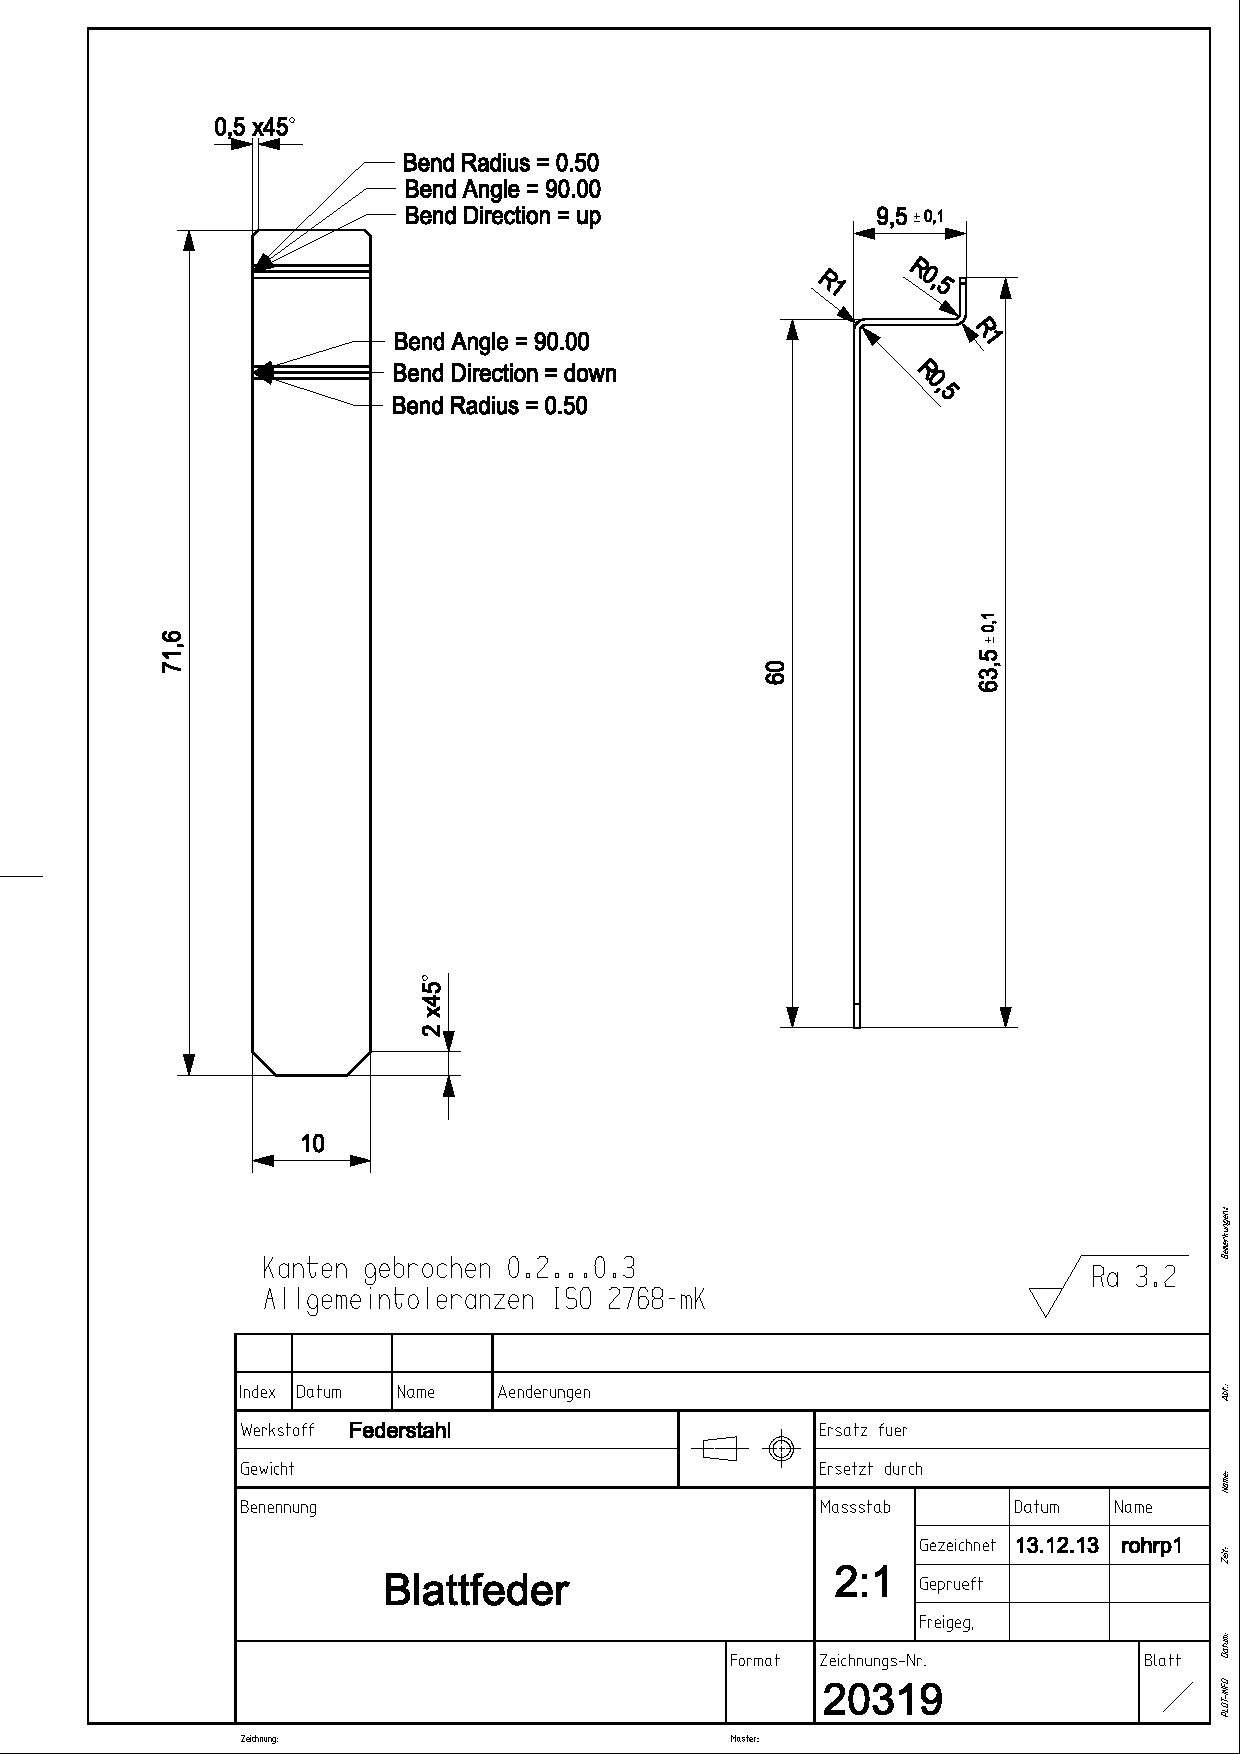
\includepdf[scale=0.7, pagecommand={}, pages=-]{appendix/image/Mammut/20319_Blattfeder.pdf}
		\includepdf[scale=0.7, pagecommand={}, pages=-]{appendix/image/Mammut/20320_Abschussblock}
		\includepdf[scale=0.7, pagecommand={}, pages=-]{appendix/image/Mammut/20321_Aufnahme_Servo.pdf}
		\includepdf[scale=0.7, pagecommand={}, pages=-]{appendix/image/Mammut/20322_Abschussrampe.pdf}
		\includepdf[scale=0.7, pagecommand={}, pages=-, landscape=true]{appendix/image/Mammut/20324_Befestigunskurve_links.pdf}
		\includepdf[scale=0.7, pagecommand={}, pages=-, landscape=true]{appendix/image/Mammut/20325_Befestigungskurve_rechts.pdf}
		\includepdf[scale=0.7, pagecommand={}, pages=-]{appendix/image/Mammut/20326_Klemme_Blattfeder.pdf}
		\includepdf[scale=0.7, pagecommand={}, pages=-, landscape=true]{appendix/image/Mammut/20327_Befestigungsplatte.pdf}
		\includepdf[scale=0.7, pagecommand={}, pages=-]{appendix/image/Mammut/20329_Hebel_Servo.pdf}
		\includepdf[scale=0.7, pagecommand={}, pages=-]{appendix/image/Mammut/20330_Klinke.pdf}
		\includepdf[scale=0.7, pagecommand={}, pages=-, landscape=true]{appendix/image/Mammut/20331_Klinkenwelle.pdf}
		\includepdf[scale=0.7, pagecommand={}, pages=-]{appendix/image/Mammut/20332_Verbindungsblock.pdf}
		\includepdf[scale=0.7, pagecommand={}, pages=-]{appendix/image/Mammut/20333_Verbindungsachse.pdf}
		\includepdf[scale=0.7, pagecommand={}, pages=-, landscape=true]{appendix/image/Mammut/20334_Lagerung_Klinkenwelle_links.pdf}
		\includepdf[scale=0.7, pagecommand={}, pages=-, landscape=true]{appendix/image/Mammut/20335_Lagerung_Klinkenwelle_rechts.pdf}
		\includepdf[scale=0.7, pagecommand={}, pages=-]{appendix/image/Mammut/20336_Drehpunktachse.pdf}
		\includepdf[scale=0.7, pagecommand={}, pages=-, landscape=true]{appendix/image/Mammut/20337_Lagerbock_Federspanner_links.pdf}
		\includepdf[scale=0.7, pagecommand={}, pages=-, landscape=true]{appendix/image/Mammut/20338_Lagerbock_Federspanner_rechts.pdf}
		\includepdf[scale=0.7, pagecommand={}, pages=-]{appendix/image/Mammut/20339_Rippe.pdf}
		\includepdf[scale=0.7, pagecommand={}, pages=-, landscape=true]{appendix/image/Mammut/20340_Explosionszeichnung_Abwurfvorrichtung.pdf}
		\includepdf[scale=0.7, pagecommand={}, pages=-]{appendix/image/Mammut/20341_Abstuetzung_links.pdf}
		\includepdf[scale=0.7, pagecommand={}, pages=-]{appendix/image/Mammut/20342_Abstuetzung_rechts.pdf}
		\includepdf[scale=0.7, pagecommand={}, pages=-]{appendix/image/Mammut/20343_Rohrbefestigung.pdf}
		%
		%
		% Netz
		\includepdf[scale=0.7, pagecommand={}, pages=-,landscape=true]{appendix/Anhang_Mechanik_PA2/Zeichnungen/Netz/20140_Netzwurfmechanismus3.pdf}
		\includepdf[scale=0.7, pagecommand={}, pages=-,landscape=true]{appendix/Anhang_Mechanik_PA2/Zeichnungen/Netz/20140_Netzwurfmechanismus2.pdf}
		\includepdf[scale=0.7, pagecommand={}, pages=-,landscape=true]{appendix/Anhang_Mechanik_PA2/Zeichnungen/Netz/20140_Netzwurfmechanismus.pdf}
		
		\includepdf[scale=0.7, pagecommand={}, pages=-,landscape=true]{appendix/Anhang_Mechanik_PA2/Zeichnungen/Netz/20110_Abschlussblech.pdf}
		\includepdf[scale=0.7, pagecommand={}, pages=-,landscape=true]{appendix/Anhang_Mechanik_PA2/Zeichnungen/Netz/20111_Netzblech.pdf}
		\includepdf[scale=0.7, pagecommand={}, pages=-]{appendix/Anhang_Mechanik_PA2/Zeichnungen/Netz/20112_Zwischenstueck.pdf}
		\includepdf[scale=0.7, pagecommand={}, pages=-]{appendix/Anhang_Mechanik_PA2/Zeichnungen/Netz/20113_Nase.pdf}
		\includepdf[scale=0.7, pagecommand={}, pages=-]{appendix/Anhang_Mechanik_PA2/Zeichnungen/Netz/20115_Fuehrungsblock.pdf}
		\includepdf[scale=0.7, pagecommand={}, pages=-]{appendix/Anhang_Mechanik_PA2/Zeichnungen/Netz/20116_Befestigungsplaettli.pdf}
		\includepdf[scale=0.7, pagecommand={}, pages=-]{appendix/Anhang_Mechanik_PA2/Zeichnungen/Netz/20117_Lagerbock.pdf}
		\includepdf[scale=0.7, pagecommand={}, pages=-]{appendix/Anhang_Mechanik_PA2/Zeichnungen/Netz/20118_Befestigungsstueck.pdf}
		\includepdf[scale=0.7, pagecommand={}, pages=-]{appendix/Anhang_Mechanik_PA2/Zeichnungen/Netz/20119_Ausloesestab.pdf}
		\includepdf[scale=0.7, pagecommand={}, pages=-]{appendix/Anhang_Mechanik_PA2/Zeichnungen/Netz/20121_Stabhalterung.pdf}
		\includepdf[scale=0.7, pagecommand={}, pages=-]{appendix/Anhang_Mechanik_PA2/Zeichnungen/Netz/20123_Befestigung_Servo.pdf}
		\includepdf[scale=0.7, pagecommand={}, pages=-]{appendix/Anhang_Mechanik_PA2/Zeichnungen/Netz/20124_Aufhaengung_Netzblech.pdf}
		\includepdf[scale=0.7, pagecommand={}, pages=-]{appendix/Anhang_Mechanik_PA2/Zeichnungen/Netz/20125_Plaettli_Aufhaenung.pdf}
		\includepdf[scale=0.7, pagecommand={}, pages=-]{appendix/Anhang_Mechanik_PA2/Zeichnungen/Netz/20126_Profilbefestigung.pdf}
		\includepdf[scale=0.7, pagecommand={}, pages=-]{appendix/Anhang_Mechanik_PA2/Zeichnungen/Netz/20127_Auflage_Netzblech.pdf}
		\includepdf[scale=0.7, pagecommand={}, pages=-]{appendix/Anhang_Mechanik_PA2/Zeichnungen/Netz/20128_Seitenblech.pdf}
		\includepdf[scale=0.7, pagecommand={}, pages=-]{appendix/Anhang_Mechanik_PA2/Zeichnungen/Netz/20129_Verbindung_Seitenblech_klein.pdf}
		\includepdf[scale=0.7, pagecommand={}, pages=-]{appendix/Anhang_Mechanik_PA2/Zeichnungen/Netz/201230_Verbindung_Seitenblech_gross.pdf}
		%
		%
		% Feuer
		\includepdf[scale=0.7, pagecommand={}, pages=-,landscape=true]{appendix/Anhang_Mechanik_PA2/Zeichnungen/Feuer/20400_Baugruppe_Feuer1.pdf}
		\includepdf[scale=0.7, pagecommand={}, pages=-,landscape=true]{appendix/Anhang_Mechanik_PA2/Zeichnungen/Feuer/20401_Baugruppe_Feuer.pdf}
		\includepdf[scale=0.7, pagecommand={}, pages=-,landscape=true]{appendix/Anhang_Mechanik_PA2/Zeichnungen/Feuer/20402_Saugeraufnahme.pdf}
		\includepdf[scale=0.7, pagecommand={}, pages=-]{appendix/Anhang_Mechanik_PA2/Zeichnungen/Feuer/20404_Servohebel_rechts.pdf}
		\includepdf[scale=0.7, pagecommand={}, pages=-]{appendix/Anhang_Mechanik_PA2/Zeichnungen/Feuer/20405_Servohebel_links.pdf}
		\includepdf[scale=0.7, pagecommand={}, pages=-]{appendix/Anhang_Mechanik_PA2/Zeichnungen/Feuer/20406_Servowelle.pdf}
		\includepdf[scale=0.7, pagecommand={}, pages=-]{appendix/Anhang_Mechanik_PA2/Zeichnungen/Feuer/20407_Servo_Lagerbock.pdf}
		\includepdf[scale=0.7, pagecommand={}, pages=-]{appendix/Anhang_Mechanik_PA2/Zeichnungen/Feuer/20408_Winkelaufnahme.pdf}
		\includepdf[scale=0.7, pagecommand={}, pages=-]{appendix/Anhang_Mechanik_PA2/Zeichnungen/Feuer/20409_Schutzklinke.pdf}
		\includepdf[scale=0.7, pagecommand={}, pages=-]{appendix/Anhang_Mechanik_PA2/Zeichnungen/Feuer/204011_Fuehrungsaufnahme.pdf}
		\includepdf[scale=0.7, pagecommand={}, pages=-,landscape=true]{appendix/Anhang_Mechanik_PA2/Zeichnungen/Feuer/204012_Saugerabdeckung.pdf}
		\includepdf[scale=0.7, pagecommand={}, pages=-]{appendix/Anhang_Mechanik_PA2/Zeichnungen/Feuer/204013_Tasteraufnahme.pdf}
		%
		%
		% Aenderungen
		\includepdf[scale=0.7, pagecommand={}, pages=-]{appendix/Anhang_Mechanik_PA2/Zeichnungen/Aenderungen/20214_Linearmodul_Grundplatte.pdf}
		\includepdf[scale=0.7, pagecommand={}, pages=-,landscape=true]{appendix/Anhang_Mechanik_PA2/Zeichnungen/Aenderungen/20327_Befestigungsplatte.pdf}
		\includepdf[scale=0.7, pagecommand={}, pages=-,landscape=true]{appendix/Anhang_Mechanik_PA2/Zeichnungen/Aenderungen/20334_Lagerung_Klinkenwelle_links.pdf}
		\includepdf[scale=0.7, pagecommand={}, pages=-,landscape=true]{appendix/Anhang_Mechanik_PA2/Zeichnungen/Aenderungen/20335_Lagerung_Klinkenwelle_rechts.pdf}
		\includepdf[scale=0.7, pagecommand={}, pages=-,landscape=true]{appendix/Anhang_Mechanik_PA2/Zeichnungen/Aenderungen/20337_Lagerbock_Federspanner_links.pdf}
		\includepdf[scale=0.7, pagecommand={}, pages=-]{appendix/Anhang_Mechanik_PA2/Zeichnungen/Aenderungen/20344_Buegel_Servo.pdf}
		\includepdf[scale=0.7, pagecommand={}, pages=-]{appendix/Anhang_Mechanik_PA2/Zeichnungen/Aenderungen/20345_Gabelhebel_Servo.pdf}
		\includepdf[scale=0.7, pagecommand={}, pages=-]{appendix/Anhang_Mechanik_PA2/Zeichnungen/Aenderungen/20346_Steg.pdf}
		\includepdf[scale=0.7, pagecommand={}, pages=-]{appendix/Anhang_Mechanik_PA2/Zeichnungen/Aenderungen/20347_Zufuehrrohr_links.pdf}
		\includepdf[scale=0.7, pagecommand={}, pages=-]{appendix/Anhang_Mechanik_PA2/Zeichnungen/Aenderungen/20348_Zufuehrrohr_rechts.pdf}
		\includepdf[scale=0.7, pagecommand={}, pages=-]{appendix/Anhang_Mechanik_PA2/Zeichnungen/Aenderungen/20349_Vereinzler_Platte.pdf}
		\includepdf[scale=0.7, pagecommand={}, pages=-]{appendix/Anhang_Mechanik_PA2/Zeichnungen/Aenderungen/20350_Vereinzler_Distanzhalter.pdf}
		\includepdf[scale=0.7, pagecommand={}, pages=-]{appendix/Anhang_Mechanik_PA2/Zeichnungen/Aenderungen/40120_Radkappe.pdf}
		\includepdf[scale=0.7, pagecommand={}, pages=-]{appendix/Anhang_Mechanik_PA2/Zeichnungen/Aenderungen/40121_Distanzscheibe.pdf}
		\includepdf[scale=0.7, pagecommand={}, pages=-]{appendix/Anhang_Mechanik_PA2/Zeichnungen/Aenderungen/40122_Distanzscheibe_Drehgeber.pdf}
		%
		
		
%Anhang E
%%%%%%%%%%%%%%%%%%%%%%%%%%%%%%%%%%%%%%%%%%%%%%%%%%%%%%%%%%%%%%%%%%%%%%%%%%%%%%%
% Titel:   Bericht - Datenbl�tter Bestellliste
% Autor:   gross10
% Datum:   13.12.2013
% Version: 0.0.1
%%%%%%%%%%%%%%%%%%%%%%%%%%%%%%%%%%%%%%%%%%%%%%%%%%%%%%%%%%%%%%%%%%%%%%%%%%%%%%%
%
%:::Change-Log:::
% Versionierung erfolgt auf folgende Gegebenheiten: -1. Release Versionen
%                                                   -2. Neue Kapitel
%                                                   -3. Fehlerkorrekturen
%
% 0.0.01      Erstellung der Datei
%%%%%%%%%%%%%%%%%%%%%%%%%%%%%%%%%%%%%%%%%%%%%%%%%%%%%%%%%%%%%%%%%%%%%%%%%%%%%%% 
\chapter{Datenbl�tter}\label{ch:datenblaetter_bestellliste}
	Datenbl�tter verwendeter Komponenten.
	\paragraph{PA1}
	\begin{itemize}
		\item drylin N-Flachf�hrungen
		\item Snap Action Switch D2F
		\item Hitec HS-5125MG
		\item Hitec HS-5645MG
	\end{itemize}
	%
	\paragraph{PA2-Mechanik}
	\begin{itemize}
		\item 
		\item 
		\item 
		\item 
		\item 
		\item 
		\item 
		\item 
		\item 
		\item 
		\item 
	\end{itemize}
	%
	\paragraph{PA2-Elektronik}
	\begin{itemize}
		\item Display: EA DOGM162x
		\item Display: NHD-0216K3Z
%		\item Display: MC21605J6W
%		\item Display: MC21605H6W
	\end{itemize}
	%
	%PA1
	\includepdf[scale=0.7, pagecommand={\thispagestyle{plain}}, pages=-]{appendix/image/f_DryLin_N_NW-02-17.pdf}
	\includepdf[scale=0.7, pagecommand={\thispagestyle{plain}}, pages=1-6]{appendix/image/f_OMRON_Sensor_D2F_1110-6257.pdf}
	\includepdf[scale=0.7, pagecommand={\thispagestyle{plain}}, pages=1]{appendix/image/f_Hitec_Servo_12mm.pdf}
	\includepdf[scale=0.7, pagecommand={\thispagestyle{plain}}, pages=1]{appendix/image/f_Hitec_RCD_Servos_Breite_18-23mm_digital_HS-5645MG_Digi.pdf}
    %
	%PA2-Mechanik
	\label{app:pa2_mech}
	\includepdf[scale=0.7, pagecommand={\thispagestyle{plain}}, pages=-]{appendix/Anhang_Mechanik_PA2/Datenblaetter/federTechnik_Groupe_Normdruckfeder_20990.pdf}
	\includepdf[scale=0.7, pagecommand={\thispagestyle{plain}}, pages=-]{appendix/Anhang_Mechanik_PA2/Datenblaetter/Festo_Steckverschraubung_QSM-M5-6.pdf}
	\includepdf[scale=0.7, pagecommand={\thispagestyle{plain}}, pages=-]{appendix/Anhang_Mechanik_PA2/Datenblaetter/Festo_Vakuumsauger_ESS_30_EN.pdf}
	\includepdf[scale=0.7, pagecommand={\thispagestyle{plain}}, pages=-]{appendix/Anhang_Mechanik_PA2/Datenblaetter/Fischereiartikel_Bernhard_Feumer_Kescher_Quik_Net.pdf}
	\includepdf[scale=0.7, pagecommand={\thispagestyle{plain}}, pages=-]{appendix/Anhang_Mechanik_PA2/Datenblaetter/Hitec_RCD_Servo_HS-7985MG.pdf}
	\includepdf[scale=0.7, pagecommand={\thispagestyle{plain}}, pages=-]{appendix/Anhang_Mechanik_PA2/Datenblaetter/Hitec_RCD_Servo_HS-8380TH.pdf}
	\includepdf[scale=0.7, pagecommand={\thispagestyle{plain}}, pages=-]{appendix/Anhang_Mechanik_PA2/Datenblaetter/iglidur_J_Druckscheibe_TypF.pdf}
	\includepdf[scale=0.7, pagecommand={\thispagestyle{plain}}, pages=-]{appendix/Anhang_Mechanik_PA2/Datenblaetter/Magnetspule_MSFG.pdf}
	\includepdf[scale=0.7, pagecommand={\thispagestyle{plain}}, pages=-]{appendix/Anhang_Mechanik_PA2/Datenblaetter/Magnetventil_MOFH.pdf}
	\includepdf[scale=0.7, pagecommand={\thispagestyle{plain}}, pages=-]{appendix/Anhang_Mechanik_PA2/Datenblaetter/Membranpumpe.pdf}
	\includepdf[scale=0.7, pagecommand={\thispagestyle{plain}}, pages=-]{appendix/Anhang_Mechanik_PA2/Datenblaetter/Minirail_DE_low.pdf}
	%
	%PA2-Elektronik
	\label{app:pa2_ele}
	\includepdf[scale=0.7, pagecommand={\thispagestyle{plain}}, pages=-]{appendix/Anhang_Bedienpanel/Display_Datasheets/dog-m.pdf}
	\includepdf[scale=0.7, pagecommand={\thispagestyle{plain}}, pages=-]{appendix/Anhang_Bedienpanel/Display_Datasheets/NHD-0216K3Z-NSW-BBW-V3.pdf}
%	\includepdf[scale=0.7, pagecommand={\thispagestyle{plain}}, pages=-]{appendix/Anhang_Bedienpanel/Display_Datasheets/1722489.pdf}
%	\includepdf[scale=0.7, pagecommand={\thispagestyle{plain}}, pages=-]{appendix/Anhang_Bedienpanel/Display_Datasheets/1722492.pdf}
%Anhang F
%%%%%%%%%%%%%%%%%%%%%%%%%%%%%%%%%%%%%%%%%%%%%%%%%%%%%%%%%%%%%%%%%%%%%%%%%%%%%%%
% Titel:   Bericht - Pflichtenheft
% Autor:   gross10
% Datum:   13.12.2013
% Version: 0.0.1
%%%%%%%%%%%%%%%%%%%%%%%%%%%%%%%%%%%%%%%%%%%%%%%%%%%%%%%%%%%%%%%%%%%%%%%%%%%%%%%
%
%:::Change-Log:::
% Versionierung erfolgt auf folgende Gegebenheiten: -1. Release Versionen
%                                                   -2. Neue Kapitel
%                                                   -3. Fehlerkorrekturen
%
% 0.0.01      Erstellung der Datei
%%%%%%%%%%%%%%%%%%%%%%%%%%%%%%%%%%%%%%%%%%%%%%%%%%%%%%%%%%%%%%%%%%%%%%%%%%%%%%% 
\chapter{Funktionstests und Testprotokolle}\label{ch:funktionstests_testprotokolle_pa2}
	F�r die mechanischen Systeme wurden entsprechende Testprotokolle und f�r die Bedienpanel ein Inbetriebnahme-Protokoll entworfen.
	\begin{itemize}
		\item Funktionstest Fresko
		\item Testprotokoll herausfallen der Bilder
		\item Funktionstest Mammut
		\item Testprotokoll Speerwerfen	
		\item Testprotokoll Speerwerfen	01.03.2014	
		\item Funktionstest Netz
		\item Testprotokoll Netzwerfen
		\item Funktionstest Feuer Fahren
		\item Inbetriebnahme-Protokoll Bedienpanel
	\end{itemize}
	%
	\includepdf[scale=0.7, pagecommand={\thispagestyle{plain}}, pages=-, landscape=false]{appendix/Anhang_Mechanik_PA2/Funktionstests/FunktionsTests_Fresko.pdf}
	\includepdf[scale=0.7, pagecommand={\thispagestyle{plain}}, pages=-, landscape=true]{appendix/Anhang_Mechanik_PA2/Funktionstests/Testprotokoll_Herausfallen_der_Bilder.pdf}
	%
	\includepdf[scale=0.7, pagecommand={\thispagestyle{plain}}, pages=-, landscape=false]{appendix/Anhang_Mechanik_PA2/Funktionstests/FunktionsTests_Mammut.pdf}
	\includepdf[scale=0.7, pagecommand={\thispagestyle{plain}}, pages=-, landscape=true]{appendix/Anhang_Mechanik_PA2/Funktionstests/Testprotokoll_Speerwerfen.pdf}
	\includepdf[scale=0.7, pagecommand={\thispagestyle{plain}}, pages=-, landscape=true]{appendix/Anhang_Mechanik_PA2/Funktionstests/Testprotokoll_Speerwerfen_01_03_2014.pdf}
	%
	\includepdf[scale=0.7, pagecommand={\thispagestyle{plain}}, pages=-, landscape=false]{appendix/Anhang_Mechanik_PA2/Funktionstests/FunktionsTests_Netz.pdf}
	\includepdf[scale=0.7, pagecommand={\thispagestyle{plain}}, pages=-, landscape=true]{appendix/Anhang_Mechanik_PA2/Funktionstests/Testprotokoll_Netzwerfen.pdf}
	%
	\includepdf[scale=0.7, pagecommand={\thispagestyle{plain}}, pages=-, landscape=false]{appendix/Anhang_Mechanik_PA2/Funktionstests/FunktionsTests_Feuer.pdf}
	%
	\includepdf[scale=0.7, pagecommand={\thispagestyle{plain}}, pages=-, landscape=true]{appendix/Anhang_Bedienpanel/Inbetriebnahmeprotokoll.png}
	%
%Anhang G
%%%%%%%%%%%%%%%%%%%%%%%%%%%%%%%%%%%%%%%%%%%%%%%%%%%%%%%%%%%%%%%%%%%%%%%%%%%%%%%
% Titel:   Bericht - Pflichtenheft
% Autor:   gross10
% Datum:   13.12.2013
% Version: 0.0.1
%%%%%%%%%%%%%%%%%%%%%%%%%%%%%%%%%%%%%%%%%%%%%%%%%%%%%%%%%%%%%%%%%%%%%%%%%%%%%%%
%
%:::Change-Log:::
% Versionierung erfolgt auf folgende Gegebenheiten: -1. Release Versionen
%                                                   -2. Neue Kapitel
%                                                   -3. Fehlerkorrekturen
%
% 0.0.01      Erstellung der Datei
%%%%%%%%%%%%%%%%%%%%%%%%%%%%%%%%%%%%%%%%%%%%%%%%%%%%%%%%%%%%%%%%%%%%%%%%%%%%%%% 
\chapter{Doxygen}\label{ch:doxygen}
	Die Doxygen-Dokumentation wird in \textsf{HTML}-Form generiert. Daher ist sie auf der beigelegten CD-ROM zu finden. Die Dokumentation umfasst nur den Stand der \gls{ac:pa1}. 
%	\includepdf[scale=0.7, pagecommand={\thispagestyle{plain}}, pages=-, landscape=true]{appendix/image/g_Funktionstest_Herausfallen_der_Bilder.pdf}
%	\includepdf[scale=0.7, pagecommand={\thispagestyle{plain}}, pages=-, landscape=true]{appendix/image/g_Funktionstest_Speerwerfen.pdf}
%	\includepdf[scale=0.7, pagecommand={\thispagestyle{plain}}, pages=-, landscape=true]{appendix/image/g_Funktionstest_Position_der_Speere_beim_Fahren.pdf}
    %\includepdf[scale=0.85, pagecommand={\thispagestyle{plain}}, pages=-]{appendix/image/b_pflichtenheft.pdf}
    %\includepdf[scale=0.85,pagecommand={\thispagestyle{plain}}, pages=-]{appendix/image/b_pflichtenheft.pdf}
%%Anhang H
%%%%%%%%%%%%%%%%%%%%%%%%%%%%%%%%%%%%%%%%%%%%%%%%%%%%%%%%%%%%%%%%%%%%%%%%%%%%%%%
% Titel:   Bericht - Pflichtenheft
% Autor:   gross10
% Datum:   13.12.2013
% Version: 0.0.1
%%%%%%%%%%%%%%%%%%%%%%%%%%%%%%%%%%%%%%%%%%%%%%%%%%%%%%%%%%%%%%%%%%%%%%%%%%%%%%%
%
%:::Change-Log:::
% Versionierung erfolgt auf folgende Gegebenheiten: -1. Release Versionen
%                                                   -2. Neue Kapitel
%                                                   -3. Fehlerkorrekturen
%
% 0.0.01      Erstellung der Datei
%%%%%%%%%%%%%%%%%%%%%%%%%%%%%%%%%%%%%%%%%%%%%%%%%%%%%%%%%%%%%%%%%%%%%%%%%%%%%%% 
\chapter{CAN Summary}\label{ch:can_summary}
	F�r die beiden Subteams Antrieb und Navigation wurde w�hrend der \gls{ac:pa2} ein Dokument zum CAN-Gatekeeper und seinen Funktionen erstellt. Die Unterlagen wurden laufend erg�nzt und entsprechen dem aktuellen Stand der Dinge. Das gesamte Summary ist als separates Dokument dieser Dokumentation beigelegt.
	%\includepdf[scale=0.8, pagecommand={}, pages=-, landscape=false]{appendix/image/i_can_summary_final.pdf}

%Anhang A
%%%%%%%%%%%%%%%%%%%%%%%%%%%%%%%%%%%%%%%%%%%%%%%%%%%%%%%%%%%%%%%%%%%%%%%%%%%%%%%%
% Titel:   Bericht - Versionierung
% Autor:   Simon Grossenbacher
% Datum:   27.09.2013
% Version: 1.0.0
%%%%%%%%%%%%%%%%%%%%%%%%%%%%%%%%%%%%%%%%%%%%%%%%%%%%%%%%%%%%%%%%%%%%%%%%%%%%%%%
%
%:::Change-Log:::
% Versionierung erfolgt auf folgende Gegebenheiten: -1. Release Versionen
%                                                   -2. Neue Kapitel
%                                                   -3. Fehlerkorrekturen
%
% 0.0.0       Erstellung der Datei
%%%%%%%%%%%%%%%%%%%%%%%%%%%%%%%%%%%%%%%%%%%%%%%%%%%%%%%%%%%%%%%%%%%%%%%%%%%%%%% 
\chapter{Versionierung}\label{ch:versionierung}
    Versionsverwaltung des vorliegenden Dokuments.
    %
    \begin{table}[htbp]
        \centering
        \begin{tabularx}{\textwidth}{|l|X|l|} 
            \hline
            \rowcolor{bfhblue}
            \textcolor{white}{Version} & \textcolor{white}{�nderung} & \textcolor{white}{Autor}\\
            \hline
            1.1.0 & PA2 Korrekturen & gross10\\
            \hline
            1.0.0 & Erste Release Version & gross10\\
            \hline
            0.0.1 & Erstellung des Dokuments & gross10 \\
            \hline
        \end{tabularx}
        \caption{Versionsverwaltung}
        \label{tab:verionsverwaltung}  
    \end{table}
%
%
%
\end{document}
